\chapter{Literature Review}\label{ch:LitReview}

\section{Context}
In order to understand my thesis, we must first understand it's context, in particular, why tracking is both critical to the operation of the receiver, as well as why it is so challenging. This chapter aims to provide a broad overview of the relationship between the material covered in this thesis, as well as it's connection to other work covered in the literature. 

\subsection{Motivation}
In order for a \ac{GPS} receiver to decode data, the carrier frequency must be tracked. This is because the data is encoded on onto the phase of the carrier signal. 

\subsection{Challenges}
Using a GPS receiver for \ac{LV} exposes the receiver to some of the most extreme circumstances imaginable. As elicited in table \ref{tab:Requirements}, we can observe that the receiver experiences velocities and accelerations far beyond what would be experienced in terrestrial applications.  The rationale behind these requirements can be found in appendix \ref{ch:FlightDynamics} and \ref{ch:Falcon9}. 
While \ac{GPS} receivers are normally used to provide provide absolute positions, the ability to provide highly accurate velocity data is incredibly valuable for spacecraft guidance. In order to insert a satellite into the proper orbit, the \ac{LV} engine-cutoff must be precisely timed, as orbital height is a function of orbital velocity. Based on analysis carried out in appendix \ref{ch:Falcon9}, we can conclude that the receiver needs to be able to provide velocity solutions which are accurate to better than 1m/s, while travelling at 6,000m/s. 

\begin{table}[!htb]
\centering
\begin{tabular}{|l|l|}
\hline
\rowcolor[HTML]{C0C0C0} 
Parameter    & Value                    \\ \hline
Altitude     & 200,000$m$                 \\ \hline
\rowcolor[HTML]{EFEFEF} 
Velocity     & 6,000$m/s$                 \\ \hline
Acceleration & 150$m/s^2$ \\ \hline
\rowcolor[HTML]{EFEFEF} 
Jerk         & 10$m/s^3$  \\ \hline
\end{tabular}
\caption{Receiver operational conditions.}
\label{tab:Requirements}
\end{table}
Unfortunately, the requirements of operation exceed the \ac{COCOM} limits, which prevent the export from the USA of GNSS receivers capable of operating:

\begin{itemize}
\item{Above 60,000ft (18,000 m)}
\item{Faster than 1,000 knots (514 m/s) }
\end{itemize}

This helps to explain the motivation to develop a receiver, which is free from \ac{COCOM} requirements.

Due to the relative motion of the satellite and the receiver, received signal differs from the transmitted carrier frequency of 1575.42 MHz due to the doppler effect\cite{Tsui}. The frequency offset due to the \ac{LOS} velocity between the receiver and the satellite can be found using \ref{eq:DopplerShift} to be 5.25Hz per m/s. Hence for the velocities experienced by \ac{LV} and \ac{SV}, we can expect doppler shifts in of 10's of Khz.

\begin{align}
\Delta f &= f_0\frac{v}{c} \text{ Hz/m/s}
\label{eq:DopplerShift}
\end{align}

Where: 
\begin{align*}
f_0 &= 1575.42 \text{ MHz}\\   
c &= 2.99792458 \times 10^8 \text{ m/s}
\end{align*}


Making reference to table \ref{tab:DopplerDynamics}, we can observe that different orders of motion have differing impacts on the doppler frequency. In figure \ref{fig:DopplerShift}, we can directly observe the effect of the receiver dynamics on the doppler shift observed by the receiver.

\begin{figure}[!htb] 
    \centering
    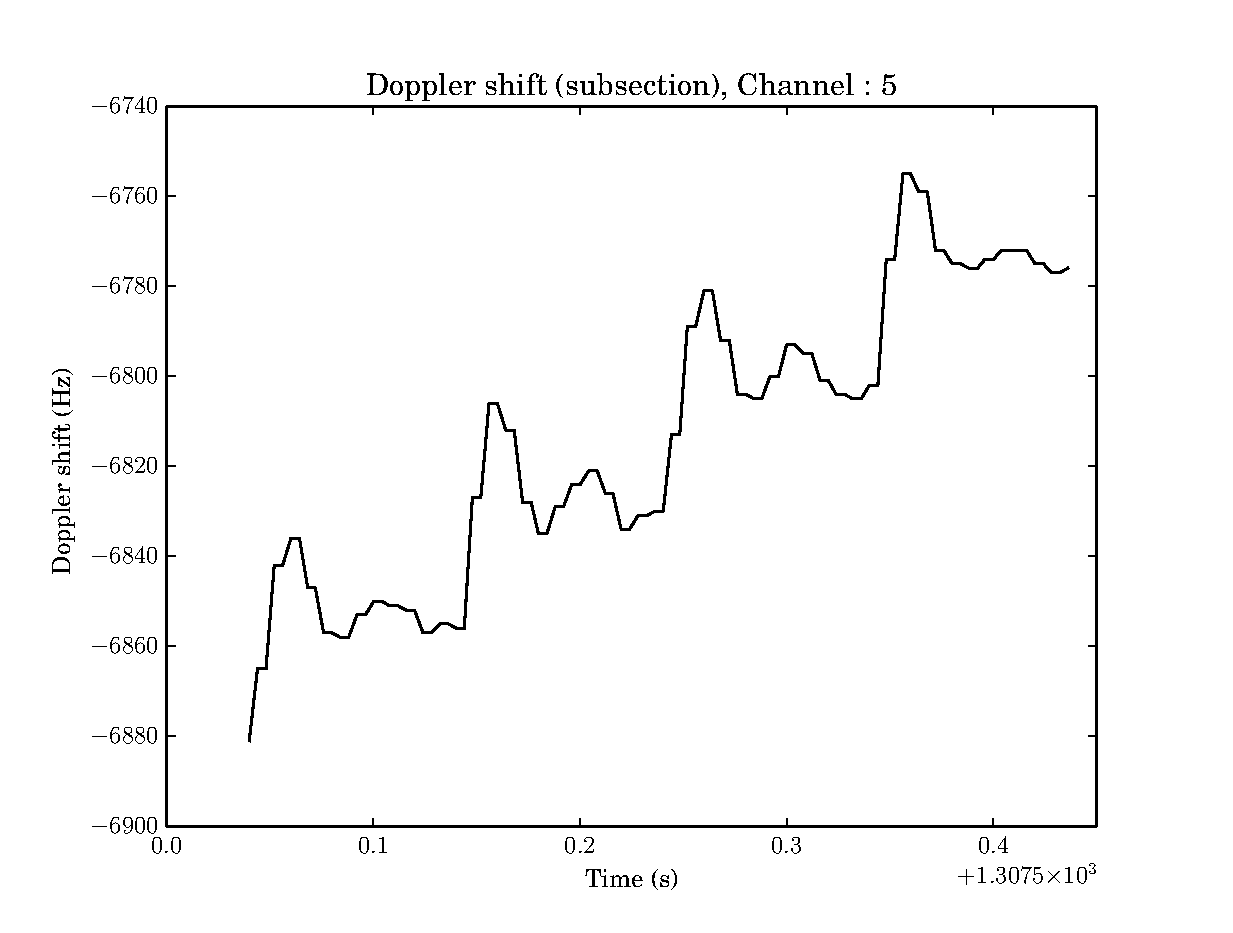
\includegraphics[width=1\textwidth]{LitReview/DopplerShift5.eps} 
    \caption{In this figure, we can observe a ramp in the doppler frequency of approximately 6,000Hz over 22.5 seconds. From this, we can conclude that the receiver is accelerating at $\approx50/s^2$.}
    \label{fig:DopplerShift}
\end{figure}


\begin{table}[!htb]
\centering
\begin{tabular}{|l|l|}
\hline
\rowcolor[HTML]{C0C0C0} 
Change in \ac{LOS} Distance & Doppler frequency \\ \hline
Static                 & 0                 \\ \hline
\rowcolor[HTML]{EFEFEF} 
Velocity               & Constant          \\ \hline
Acceleration           & Ramp              \\ \hline
\rowcolor[HTML]{EFEFEF} 
Jerk                   & Parabolic         \\ \hline
\end{tabular}
\caption{The relationship between \ac{LOS} dynamics and Doppler frequency.}
\label{tab:DopplerDynamics}
\end{table}

Turning our attention to the motion of the GPS satellite, Tsui states that the maximum line of sight velocity for a stationary receiver due to the motion of the satellite is $\approx 929 m/s$, or 4.9KHz. Finally, it is important to note that the maximum \ac{LOS} acceleration due to the motion of the satellite is $\approx 0.188m/s^2$, or 0.936 Hz/s\cite{Tsui}. From this, we can conclude that the \ac{LOS} dynamics are dominated by the motion of the receiver.

\section{Introduction to PLLs}
PLLs are a versatile tool for solving many problems in electrical engineering, hence there is a significant body of literature which relates to the design, implementation and applications of PLLs. 

One of the most beautiful properties of a PLL, is that once it has locked onto an incoming signal, then the average frequency of the local replica is exactly equal to the average frequency of the incoming signal. We can understand why this is true, as if the average frequency of the local replica of was different to the average frequency of the incoming signal, than the phase error would increase over time, and eventually the loop would loose lock. This property can be exploited in order to provide an highly accurate estimate of the velocity of the receiver based on the doppler shift in frequency. As alluded to before, the receiver needs to be able to provide velocity solutions which are accurate to better than 1m/s, or 5.25Hz of doppler shift. It is important to remember that phase lock does not imply zero phase error, or zero instantaneous velocity error\cite{Gardner}. 

\tikzset{
block/.style = {draw, fill=white, rectangle, minimum height=3em, minimum width=3em},
tmp/.style  = {coordinate}, 
sum/.style= {draw, fill=white, circle, node distance=1cm},
input/.style = {coordinate},
output/.style= {coordinate},
pinstyle/.style = {pin edge={to-,thin,black}
}
}

\begin{figure}[!htb]
\centering
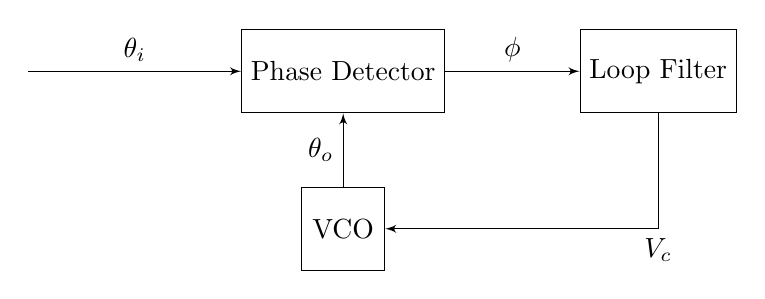
\begin{tikzpicture}[auto, node distance=4cm,>=latex']
    \node [input, name=rinput] (rinput) {};
    
    
    \node [block, right of=rinput](PhaseDetector){Phase Detector};
    
    \node [block, right of=PhaseDetector] (LoopFilter) {Loop Filter};
    
    \node [block, below of = PhaseDetector,node distance = 2
    cm](VCO){VCO};
    
    \draw [->] (rinput) -- node{$\theta_{i}$} (PhaseDetector);
    \draw [->] (PhaseDetector) -- node{$\phi$} (LoopFilter);
    \draw [->] (LoopFilter) |- node{$V_{c}$} (VCO);
    \draw [->] (VCO) -- node{$\theta_{o}$} (PhaseDetector);
    
    \end{tikzpicture}
\caption{An abstracted diagram of a typical PLL.} 
\label{fig:PLLAnalog}
\end{figure}


Every PLL contains 3 key components,

\begin{itemize}
\item{Phase Detector}
\item{Loop Filter}
\item{Oscillator}
\end{itemize}

In figure \ref{fig:PLLAnalog} we can observe relationship between these components. The \emph{Phase Detector} measures the phase between difference an incoming signal $\omega_{input}$ and an internally generated signal $\omega_{local}$, generating the error signal, which is ideally equal to $\theta_i -\theta_o$. This error signal is then filtered by the \emph{Loop Filter}, which generates a control signal as well as  removes noise and high frequency components. This control signal is then used by the \emph{\ac{VCO}} to generate $\omega_{local}$. The \ac{VCO} acts as an integrator, because phase is the integral of frequency with respect to time. The focus of this thesis is the loop filter, which as Gardner points out, can be more aptly be thought of as a loop controller\cite{Gardner}. This is because of the role of the loop filter in establishing the dynamics of the feedback loop and generating a control signal for the VCO\cite{Kaplan}.

TALK MORE ABOUT THIS
\begin{equation}
	\omega_{VCO} = \omega_0 + K_{VCO}V_{LF}
\end{equation}

Where:
\begin{align*}
	\omega_0 &= \text{The VCO centre frequency}\\
	K_{VCO} &= \text{The VCO gain}\\
\end{align*}


\begin{figure}[!htb]
\centering

\usetikzlibrary{shadows,arrows}
% Define the layers to draw the diagram
\pgfdeclarelayer{background}
\pgfdeclarelayer{foreground}
\pgfsetlayers{background,main,foreground}
 
% Define block styles  
\tikzstyle{materia}=[draw, fill=blue!20, text width=6.0em, text centered,
  minimum height=1.5em,drop shadow]
\tikzstyle{Lab} = [materia, text width=8em, minimum width=10em,
  minimum height=3em, rounded corners, drop shadow]
\tikzstyle{texto} = [above, text width=6em, text centered]
\tikzstyle{linepart} = [draw, thick, color=black!50, -latex', dashed]
\tikzstyle{line} = [draw, thick, color=black!50, -latex']
\tikzstyle{ur}=[draw, text centered, minimum height=0.01em]
 
% Define distances for bordering
\newcommand{\blockdist}{1.3}
\newcommand{\edgedist}{1.5}
\newcommand{\myBlock}[2]{node (p#1) [Lab]{#2}}

% Draw background
\newcommand{\background}[5]{%
  \begin{pgfonlayer}{background}
    % Left-top corner of the background rectangle
    \path (#1.west |- #2.north)+(-0.5,0.5) node (a1) {};
    % Right-bottom corner of the background rectanle
    \path (#3.east |- #4.south)+(+0.5,-0.25) node (a2) {};
    % Draw the background
    \path[fill=yellow!20,rounded corners, draw=black!50, dashed]
      (a1) rectangle (a2);
    \path (a1.east |- a1.south)+(0.8,-0.3) node (u1)[texto]
      {\scriptsize\textit{Unidad #5}};
  \end{pgfonlayer}}

\newcommand{\transreceptor}[3]{%
  \path [linepart] (#1.east) -- node [above]
    {\scriptsize Transreceptor #2} (#3);}

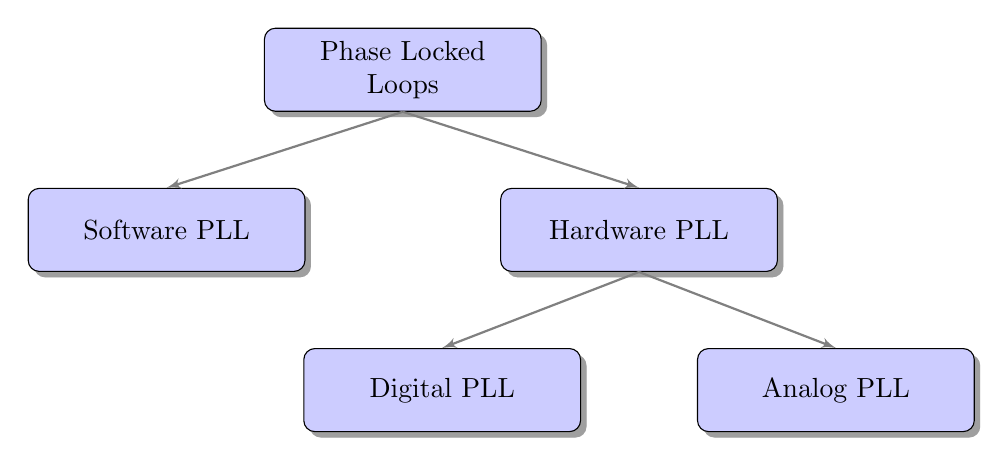
\begin{tikzpicture}[transform shape]
 
 % Draw diagram elements
  \path \myBlock {1}{Phase Locked Loops};
  \path (p1.south)+(-3,-1.5) \myBlock{2}{Software PLL};
  \path (p1.south)+(3,-1.5) \myBlock{3}{Hardware PLL};
  \path (p3.south)+(2.5,-1.5) \myBlock{4}{Analog PLL};
  \path (p3.south)+(-2.5,-1.5) \myBlock{5}{Digital PLL};
     
  % Draw arrows between elements
  \path [line] (p1.south) -- node  {} (p2.north);
  \path [line] (p1.south) -- node  {} (p3.north);
  \path [line] (p3.south) -- node  {} (p4.north);
  \path [line] (p3.south) -- node  {} (p5.north);

\end{tikzpicture}
\caption{A taxonomy of PLLs \cite{Best}}
\label{fig:Taxonomy}
\end{figure}

At this stage, it is important to elaborate on the taxonomy of PLLs, which can be visualised in figure \ref{fig:Taxonomy} and table \ref{tab:PLLTaxonomy}. The Namuru utilises a Software PLL, which is implemented in the C programing language on one of processor cores. However, in order to understand the operation and performance of the PLL, we analyse it as an Analog PLL. While every PLL is inherently non-linear, Gardner states that "Tools for analysis of nonlinear systems are exceedingly cumbersome and provide merger benefits compared to the powerful analytical tools available for linear systems". Gardner consistently states that linear methods are sufficient for the bulk of analysis and design of most PLLs, and therefore linear approximations should be employed wherever feasible\cite{Gardner}. 

\begin{table}[!htb]
\centering
\begin{tabular}{|l|l|l|l|}
\hline
\rowcolor[HTML]{C0C0C0} 
\begin{tabular}[c]{@{}l@{}}PLL Category\end{tabular}            & Phase Detector & Phase Error Signal & Loop Filter \\ \hline
\begin{tabular}[c]{@{}l@{}}LPLL (Linear PLL)\end{tabular}       & Analog         & Analog             & Analog      \\ \hline
\rowcolor[HTML]{EFEFEF} 
\begin{tabular}[c]{@{}l@{}}DPLL (Digital PLL)\end{tabular}      & Digital        & Analog             & Analog      \\ \hline
\begin{tabular}[c]{@{}l@{}}ADPLL (All Digital PLL)\end{tabular} & Digital        & Digital            & Digital     \\ \hline
\rowcolor[HTML]{EFEFEF} 
\begin{tabular}[c]{@{}l@{}}SPLL (Software PLL)\end{tabular}     & Software       & Software           & Software    \\ \hline
\end{tabular}
\label{tab:PLLTaxonomy}
\caption{A taxonomy of PLLs\cite{ADPLL,Best}.}
\end{table}

\clearpage

\section{Analog PLLs}

Analog PLLs provide a useful abstraction for the development and analysis of Digital PLLs. A common method of developing PLLs for \ac{GPS} receivers is to design the control loop in the Laplace (analog) domain, and convert it to the discrete (digital) domain. 

\begin{figure}[!htb] 
    \centering
    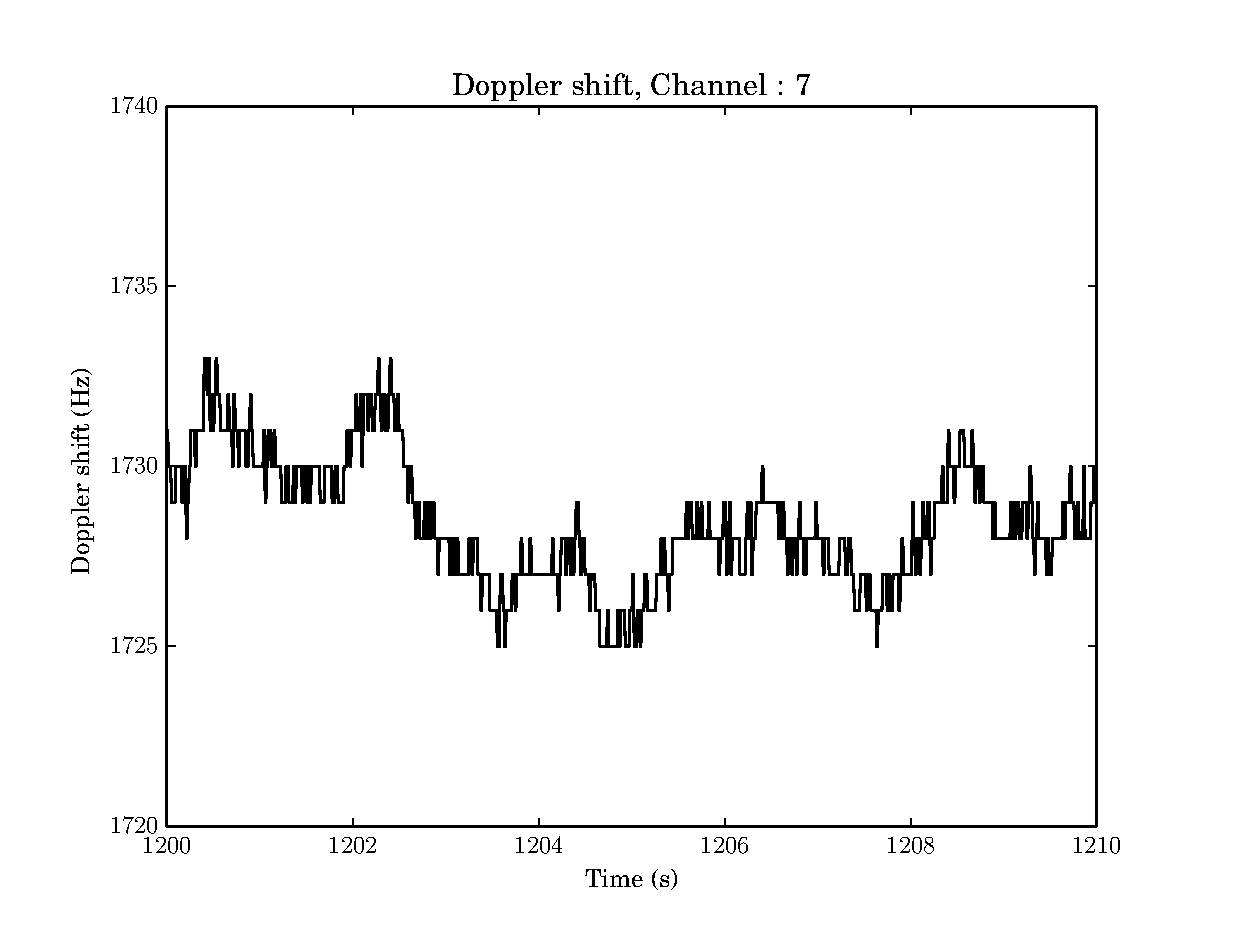
\includegraphics[width=1\textwidth]{LitReview/DopplerShift7.eps} 
    \caption{The raw output from the receiver while it is operating over a 10 second period. 
    The receiver is stationary, and tracking a live satellite.}
    \label{fig:DopplerShiftStationary}
\end{figure}

\begin{figure}[!htb] 
    \centering
    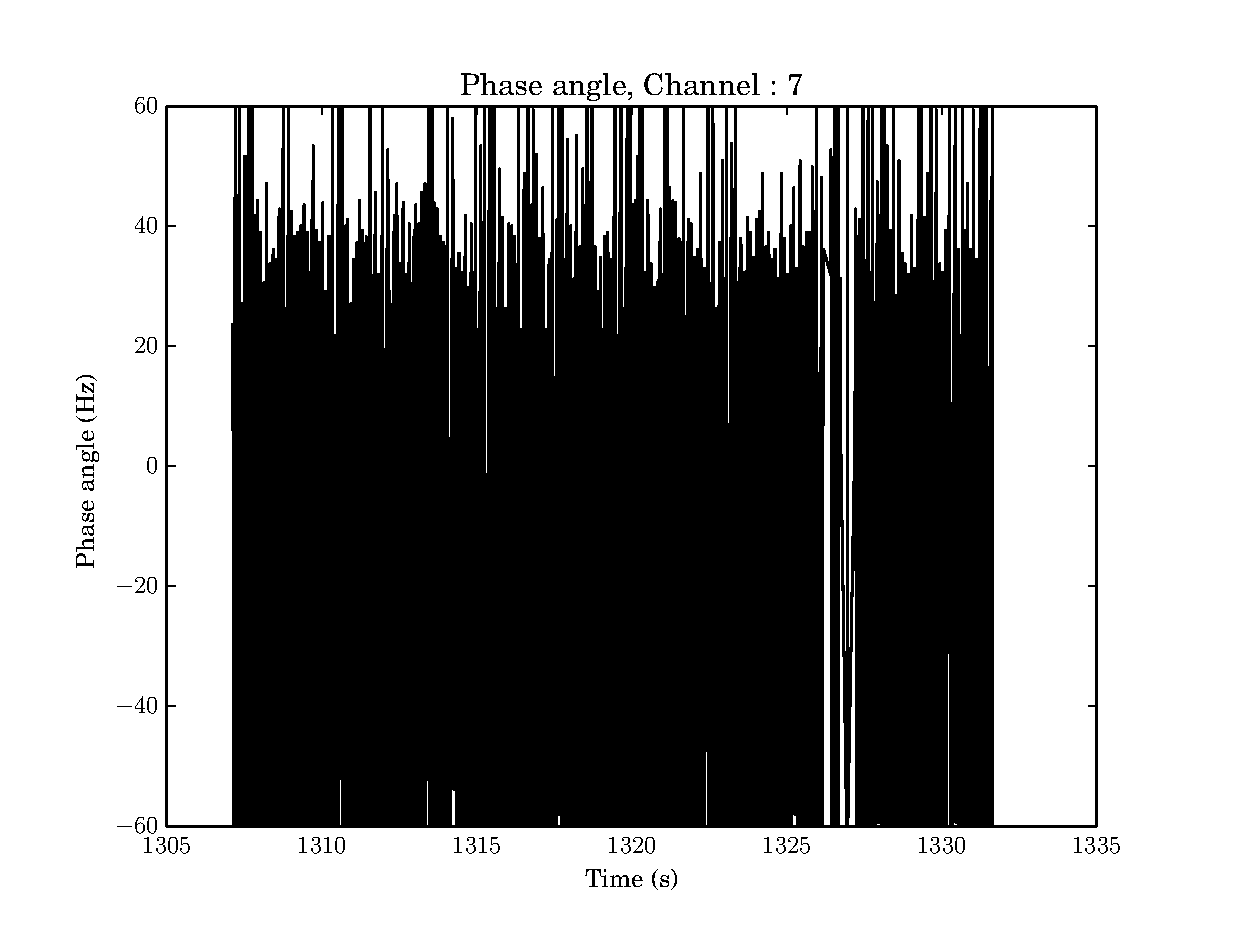
\includegraphics[width=1\textwidth]{LitReview/PhaseAngle7.eps} 
    \caption{The phase angle at the output from the phase detector while tracking the signal in figure \ref{fig:DopplerShiftStationary}. Note that the signal is zero mean.}
    \label{fig:PhaseAngleStationary}
\end{figure}

\begin{figure}[!htb] 
    \centering
    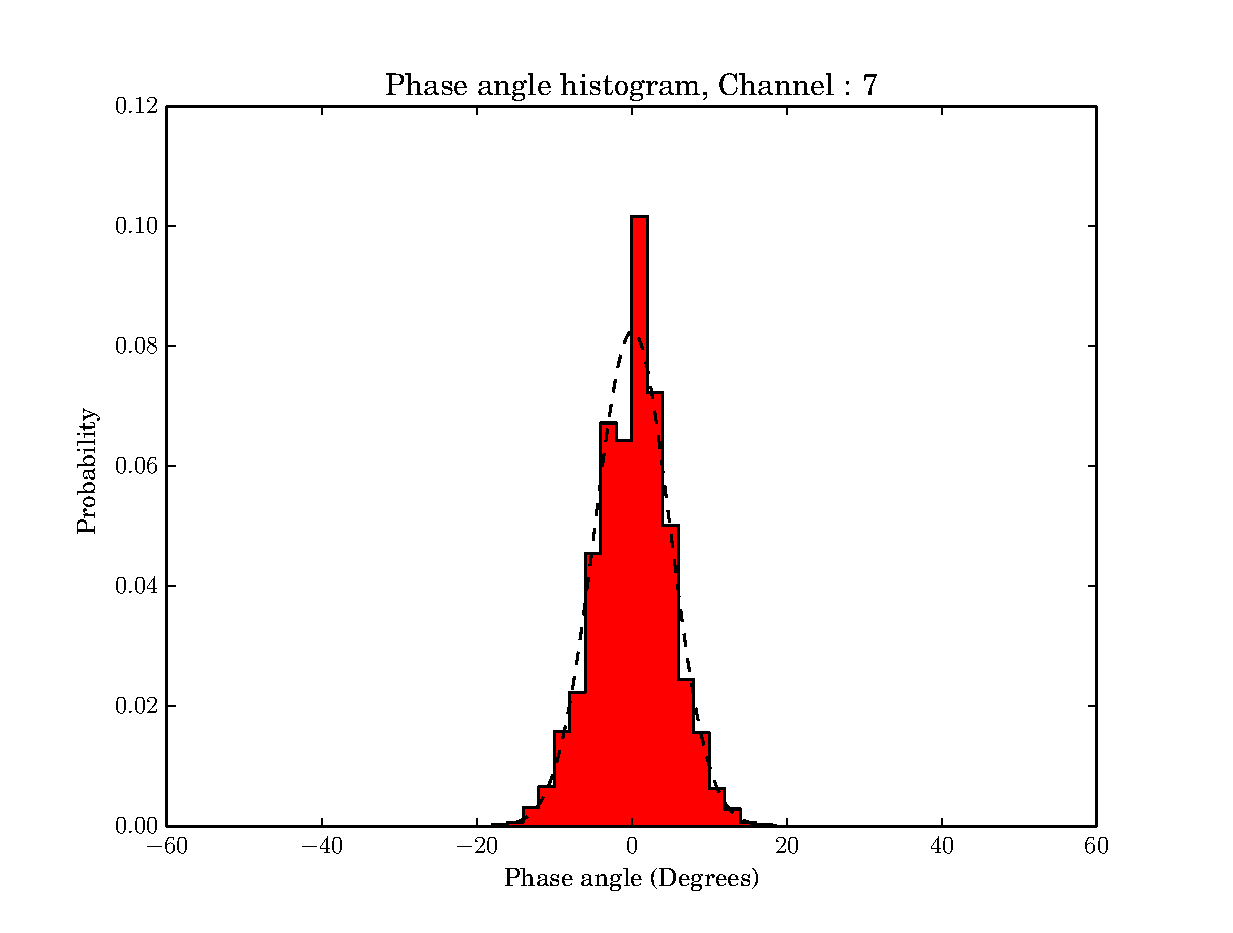
\includegraphics[width=1\textwidth]{LitReview/PhaseAngleHistogram7.eps} 
    \caption{A histogram of the phase angle from plot \ref{fig:PhaseAngleStationary}. A normal distribution with the 
    same mean and standard deviation ($4.83\degree$) as the phase angle signal is overlaid. As will be discussed later, the standard deviation, $\sigma$ of the phase error is a crucial statistic in understanding the performance of a PLL tracking loop.}
    \label{fig:PhaseAngleHistogramStationary}
\end{figure}

	\subsection{Loop type}
    The choice of loop type is arguably the single most important choice that must be made
    during the design the tracking loops. The nomenclature of the term "loop type" is borrowed from control theory, 
    and refers to the number of integrators in the loop\cite{Gardner}. Because the \ac{VCO} is in effect an integrator,
    the order of a PLL is always at least 1. 
    
    From table \ref{tab:DopplerDynamics} we can see that the order of the dynamics the receiver
    experiences has and impact on the order of the doppler shifts that will be seen by the receiver. Appendix \ref{ch:FlightDynamics}
    and \ref{ch:Falcon9} exhaustively analyse the dynamics that the \ac{LV} will experience, however in summary, the receiver will experience:
    
    \begin{enumerate}
    \item{Extreme velocities}
    \item{Persistent, significant acceleration}
    \item{Significant jerk}
    \end{enumerate}
    
    From table \ref{tab:LoopOrders} we can observe what order of dynamics different loop types are sensitive to. Ultimately, a trade-off exists between filter order and stability. Type 1 \& 2 filters are unconditionally stable in the Laplace domain, however they are not as effective as third order loops at coping with dynamics. For example, the residual error of a type 2 loop is acceleration. This makes it unsuitable for any application where sustained acceleration is likely to be encountered, as the error will increase over time, until phase lock is lost. However, type 2 are effectively insensitive to velocity, this is because the integrator in the loop filter contains and estimate of the doppler shift due the current velocity. In most real world scenarios, sustained acceleration is limited, due to limits on maximum achievable velocities. For space based applications however, velocities of thousands of meters per second are routinely achieved. Hence while a type 2 loop may be suitable for terrestrial applications, a type 3 loops is required for spaced based applications. A type 3 loop is insensitive to acceleration and velocity, because the loop filter contains a pair of integrators. One of the integrators contains an estimate of the current velocity, the other of the current acceleration\cite{Kaplan}. 
    
    \begin{table}[!htb]
\centering
\begin{tabular}{|l|l|l|l|}
\hline
\rowcolor[HTML]{C0C0C0} 
Loop order & Filter order & Characteristics & Stability                               \\ \hline
1          & 0            & Sensitive to velocity stress       & Unconditionally stable                                  \\ \hline
\rowcolor[HTML]{EFEFEF} 
2          & 1            & Sensitive to acceleration stress   & Unconditionally stable                                   \\ \hline
3          & 2            & Sensitive to jerk stress          & Stable for $B_n$ \textless 18 Hz \\ \hline
\end{tabular}
\caption{Loop order behaviour. Note that the stability of the type 3 loop is predicated on a 20ms coherent integration time/update rate. The \ac{NAMURU} receiver uses an 8ms update rate, so the relevant loop bandwidth is 45Hz. Table from Kaplan\cite{Kaplan}.}
\label{tab:LoopOrders}
\end{table}

    
	\subsection{Stresses}
		\subsubsection{Thermal}
		\subsubsection{Dynamics}
		\ref{ch:FlightDynamics}
		\ref{ch:Falcon9}
		\subsubsection{Vibration}
		\ref{ch:Vibration}

    \subsection{Noise Bandwidth}
    
    
	\subsection{Loop coefficients}
	The determination of loop coefficients has been the subject of significant effort in the literature.  While the choice of loop type is relatively straightforward, and dictated by the application, the selection of appropriate coefficients for the loop filter is somewhat more nuanced. Hence, a the focus of this thesis has been on critically analysing the loop coefficients used in the current \ac{NAMURU} receiver. 
	
	Kaplan describes the loop filters objective as reducing noise, in order to produce an accurate estimate of the original signal\cite{Kaplan}. Gardner on the other hand takes a subtly different view, choosing to focus more on the loop filters ability to regulate the output signal dynamics\cite{Gardner}. Again, it is important to recall at this point that the terms loop filter and loop controller are synonymous. 
	
	
	The \ac{NAMURU} receiver uses a number of different PLL's while in different operational states. The relationship between the different types of PLL's used as further analysis is carried out in appendix \ref{ch:StateTransitions} and \ref{ch:LaplaceAnalysis}. The state that will receive the most thorough analysis in this thesis is the type 3 PLL. 
	
	
	From Gardner, we find that we can require 3 independent parameters in order to characterise the PLL\cite{Gardner}. In equation \ref{eq:3rdOrderLoop}, we can observe the presence of $s^3$ in the denominator, confirming that this is a type 3 loop. The factor of $\frac{1}{s}$ is the integrator inside the \ac{VCO}.
	
	
	\begin{equation}
	G(s) = \frac{1}{s}(1 + \frac{K_2}{K_1s} + \frac{K_3}{K1s^2})
	\label{eq:3rdOrderLoop}
	\end{equation}
	
	
	The design method which was used to originally design \ac{NAMURU} is described by Ward and Kaplan, \cite{Ward},\cite{Kaplan}, and relies on designing the PLL in the Laplace (analog) domain, and then transforming into the digital domain for implementation. The method developed by Ward enjoys significant popularity, in part because it develops relatively robust designs, based on proven rules of thumb. The design process used will be described in more comprehensive detail in chapter \ref{ch:MyWork}, however it is important to recognise other design methods that exist. 
	
    
    
    
	\subsection{Transient response}
	
	\subsection{Stability}

\clearpage

\section{Digital PLL's}
	\subsection{Bilinear vs Boxcar}
	\subsection{Stability}
	\subsection{Transient response}




%Flight Dynamics
%\addcontentsline{toc}{chapter}{Appendix 1}\label{app1}
\chapter{Flight Dynamics}

\section{Overview}
In order to design a receiver able to cope with high dynamics experienced during space flight, it is crucial to have an understanding of the types of dynamics the receiver is likely to occur. Based on a thorough analysis of a range of Launch Services User's Guide published by commercial space flight operators, the following phases of flight have been identified as exhibiting the most severe dynamics: 

\begin{enumerate}
\item{Launch}
\item{Stage Separation}
\item{Re-entry}
\end{enumerate}

\subsection{Launch}
Launch is the most obvious case of dynamics that a \ac{GNSS} receiver would experience. Axial accelerations of 6 g are experienced with most launch vehicles, up to 13 g in the case of the Minotaur rocket. During ascent, accelerations of 2 g due to crosswinds and course corrections may be experienced. An overview of the launch dynamics experience by a range of acceleration that a \ac{SV} will experience can be found in table \ref{QSLTable}.

\begin{figure}[!htb] 
    \centering
    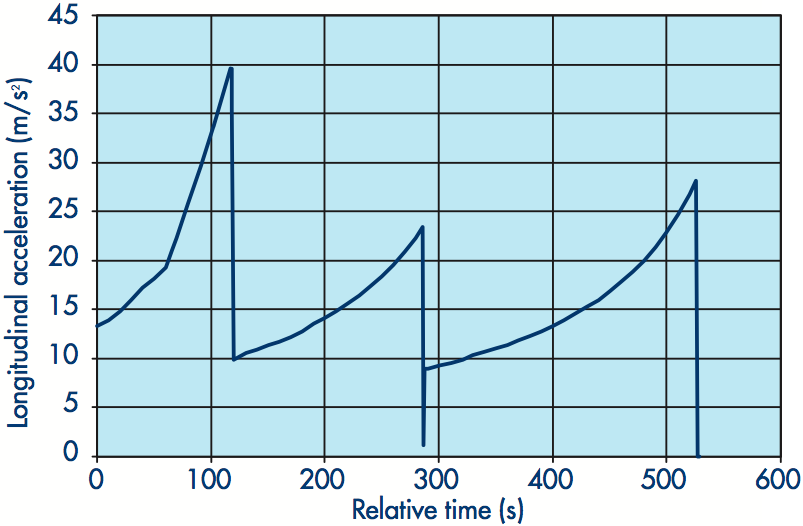
\includegraphics[width=1\textwidth]{FlightDynamics/SoyuzAcceleration.png} 
    \caption{Typical longitudinal acceleration experienced by the Soyuz payload. Note the significant change in acceleration (Jerk) upon stage separation. Image from \cite{Soyuz}}
    \label{fig:SoyuzAcceleration}
\end{figure}

\begin{figure}[!htb] 
    \centering
    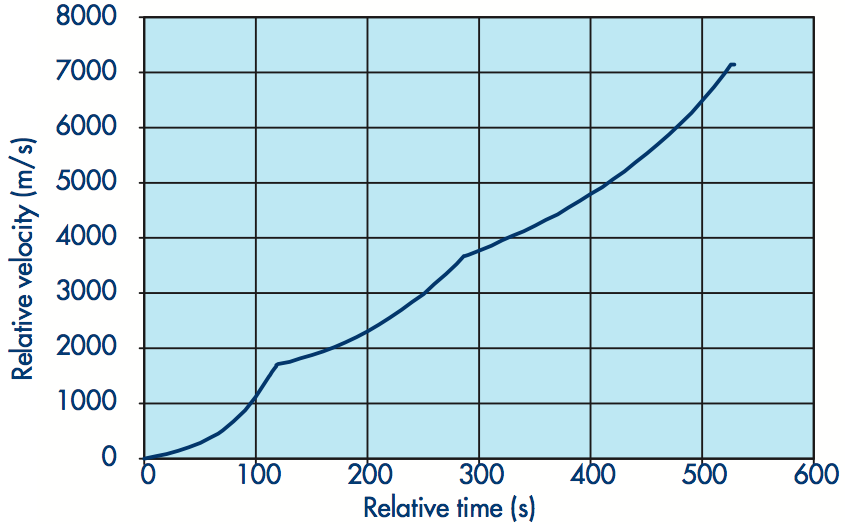
\includegraphics[width=1\textwidth]{FlightDynamics/SoyuzRelativeVelocity.png} 
    \caption{Typical Soyuz velocity. Image from \cite{Soyuz}}
    \label{fig:SoyuzRelativeVelocity}
\end{figure}



\begin{table}[!htb]
\centering
\begin{tabular}{|l|l|l|}
\hline
\rowcolor[HTML]{C0C0C0} 
Space Vehicle       & Axial                   & Lateral                \\ \hline
Ariane 5            & 4.6 g \cite{Ariane}     & 2.0 g \cite{Ariane}    \\ \hline
\rowcolor[HTML]{EFEFEF} 
Atlas V 400         & 5.0 g \cite{AtlasV}     & 2.0 g \cite{AtlasV}    \\ \hline
Atlas V 500         & 4.6 g \cite{AtlasV}     & 2.0 g \cite{AtlasV}    \\ \hline
\rowcolor[HTML]{EFEFEF} 
Delta IV Medium     & 6.0 g \cite{DeltaIV}    & 2.0 g \cite{DeltaIV}   \\ \hline
Delta IV Heavy      & 5.5 g \cite{DeltaIV}    & 2.0 g \cite{DeltaIV}   \\ \hline
\rowcolor[HTML]{EFEFEF} 
Falcon 9 Revision 0 & 6.0 g \cite{Falcon9}    & 2.0 g \cite{Falcon9}   \\ \hline
Minotaur            & 13.0 g  \cite{Minotaur} & 12.0 g \cite{Minotaur} \\ \hline
\rowcolor[HTML]{EFEFEF} 
Soyuz               & 5.0 g \cite{Soyuz}      & 1.8 g \cite{Soyuz}     \\ \hline
\end{tabular}
\caption{Maximum \ac{QSL} experienced during launch.}
\label{QSLTable}
\end{table}



\subsection{Stage Separation}

Significant shocks can be generated during stage separation, due to pyrotechnic events and fairing jettison\cite{AtlasV,Ariane,DeltaIV}. While these shocks have no impact on the line of sight dynamics experienced by the receiver, they do have an impact on the crystal. Mechanical vibrations can modulate the output frequency of the crystal, placing stress on the tracking loops. A mission profile for a Minotaur rocket can be seen in figure \ref{fig:MinotaurMissionProfile}.


\begin{figure}[!htb] 
    \centering
    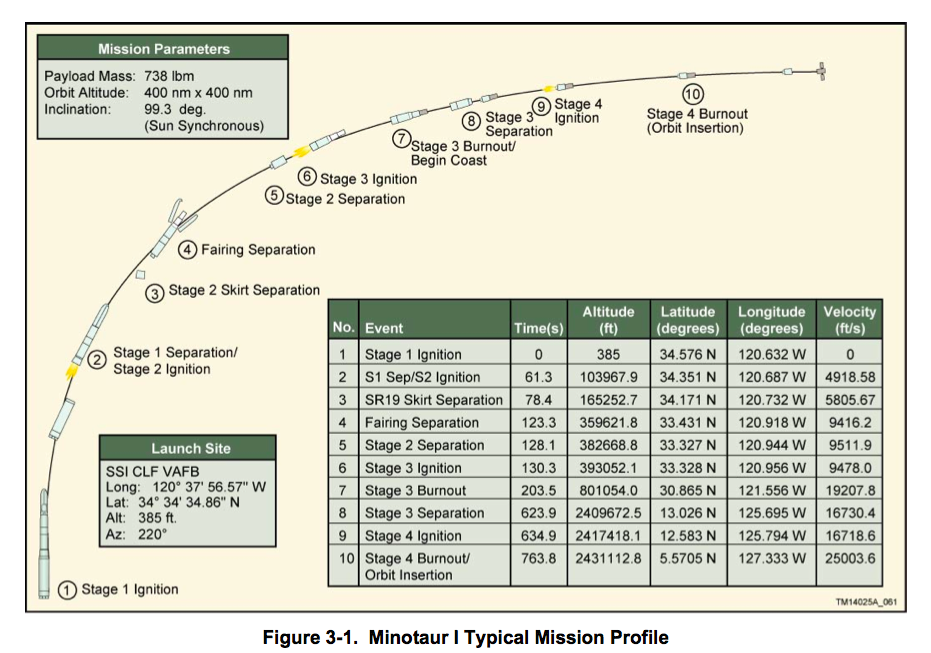
\includegraphics[width=1\textwidth]{FlightDynamics/MinotaurMissionProfile.png} 
    \caption{A typically Minotaur mission profile, note there are 5 unique separation events. Image from \cite{Minotaur}}
    \label{fig:MinotaurMissionProfile}
\end{figure}

\subsection{Re-entry}
Getting to space is only half the challenge. Accurate guidance during re-entry is crucial to reducing costs in the space industry. Most \ac{SV}'s are currently employed to launch satellites, however manned missions regularly return capsules to earth. The maximum design acceleration experienced can be seen in table \ref{ReEntryTable}. 

During re-entry, the extreme temperatures ionises the gasses surrounding the vehicle, forming  layer of plasma. This layer of plasma severely attenuates radio signals, resulting in what is termed 'reentry blackout'. GNSS receiver design presents an inherent trade off between sensitivity and high dynamics performance. It is likely that the receiver will loose track of the the signal, and be forced to re-acquire at a lower altitude, once the plasma has subsided. 


\begin{table}[!htb]
\centering
\begin{tabular}{|l|l|}
\hline
\rowcolor[HTML]{C0C0C0} 
Space Vehicle & Peak acceleration                    \\ \hline
Gemini        & 12 g \cite{FAA}                      \\ \hline
\rowcolor[HTML]{EFEFEF} 
Apollo        & 7.19 g \cite{johnston1975biomedical} \\ \hline
Dragon        & 5.0 g \cite{trevino2008spacex}       \\ \hline
\rowcolor[HTML]{EFEFEF} 
Soyuz         & 10 g \cite{ReentryDynamics}          \\ \hline
\end{tabular}
\caption{Peak acceleration experienced by different \ac{SV}'s during re-entry}
\label{ReEntryTable}
\end{table}



Space Exploration Technologies Corporation (SpaceX) is attempting to reduce launch costs by recovering the first stage of their Falcon 9-R launch vehicle. After first stage separation, the first stage performs a burn-back procedure, to fly back to the launch pad. During the burn-back, there is an inferred maximum de-acceleration of $\approx 7.8 g$ during the hypersonic burn, based on published performance figures. An overview of the flight profile can be found in figure \ref{fig:Falcon9Profile}.

\begin{figure}[!htb] 
    \centering
    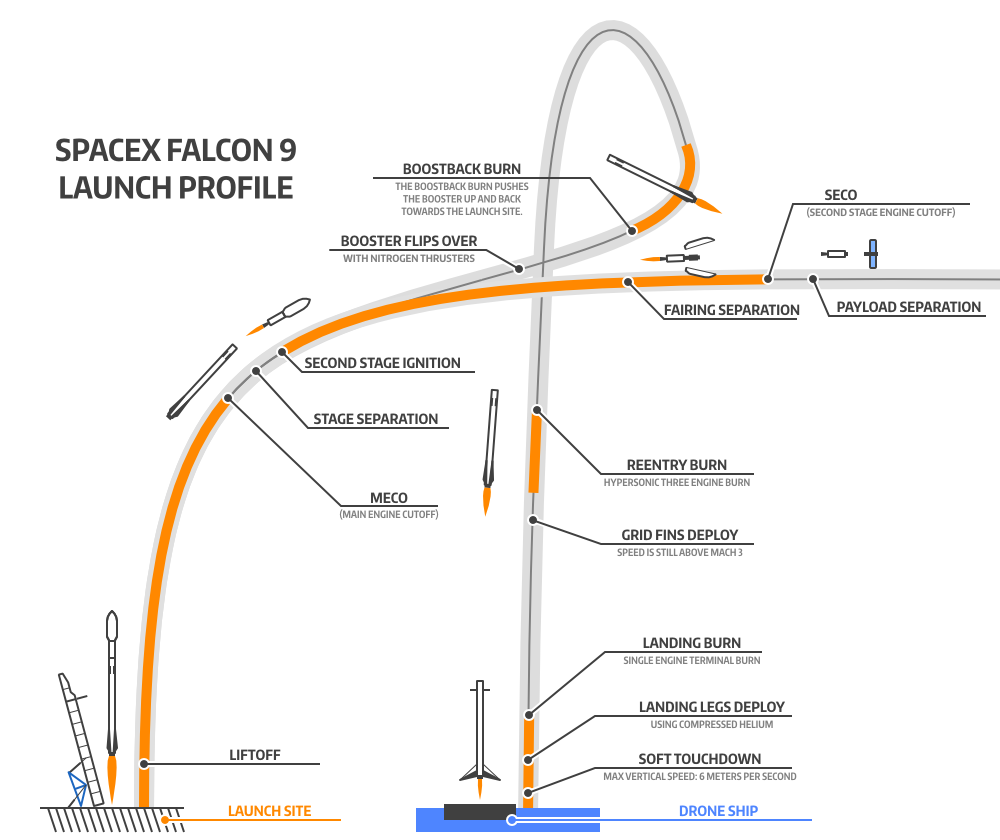
\includegraphics[width=1\textwidth]{FlightDynamics/Falcon9Profile.png} 
    \caption{An overview of the Falcon 9-R flight profile.}
    \label{fig:Falcon9Profile}
\end{figure}


The maximum acceleration experienced during re-entry can be closely approximated parametrically using the following equation from \cite{eastre}. This is convenient, as it provides an intuitive understanding of how the maximum acceleration varies with velocity, as well as allowing performance to be estimated, when official figures are not published. : 
$$(\frac{dv}{dt})_{max} = -\frac{\beta V_0 ^2}{2e} \sin \gamma_0$$

$\beta$ = atmospheric scale height, a parameter used to describe the density profile of the atmosphere = $0.000139 m^-1$ for Earth

$\gamma$ = vehicle's flight-path angle (deg or rad)

e = base of the natural logarithm = 2.7182\ldots

%Laplace Analysis
%\addcontentsline{toc}{chapter}{Appendix 2}\label{app2}
\chapter{Laplace Analysis}

\emph{"All models are wrong, but some are useful" -George E. P. Box}


\begin{table}[!htb]
\resizebox{\textwidth}{!}{%
\begin{tabular}{@{}llll@{}}
\toprule
Name     & Physical interpretation & Time function    & Laplace transform \\ \midrule
Step     & Constant position       & $1$              & $\frac{1}{S}$     \\\addlinespace[5pt]
Ramp     & Constant velocity       & $t$              & $\frac{1}{S^2}$   \\\addlinespace[5pt]
Parabola & Constant acceleration   & $\frac{1}{2}t^2$ & $\frac{1}{S^3}$  \\\addlinespace[5pt]
\end{tabular}
}
\caption{Test inputs for evaluating errors \cite{Nise}}
\label{tab:LaplaceTestInputs}
\end{table}


\tikzset{
block/.style = {draw, fill=white, rectangle, minimum height=3em, minimum width=3em},
tmp/.style  = {coordinate}, 
sum/.style= {draw, fill=white, circle, node distance=1cm},
input/.style = {coordinate},
output/.style= {coordinate},
pinstyle/.style = {pin edge={to-,thin,black}
}
}

\begin{figure}[!htb]
\centering
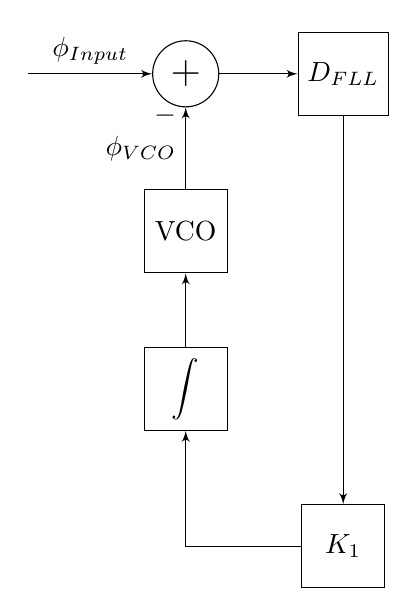
\begin{tikzpicture}[auto, node distance=2cm,>=latex']
    \node [input, name=rinput] (rinput) {};
    \node [sum, right of=rinput,node distance = 2
    cm](Rotator){\Large$+$};
    
    %FLL Stuff
    \node [block, right of=Rotator,node distance=2cm] (DiscriminatorFLL) {$D_{FLL}$};
    
    \node [block, below of = DiscriminatorFLL,node distance =6cm](K1FLL){$K_{1}$};
    
    \node [block, below of = Rotator](VCO){VCO};
    \node [block, below of = VCO](VCOIntegrator){$\displaystyle \int$};
    
    
    %Common
    \draw [->] (rinput) -- node{$\phi_{Input}$} (Rotator);
    
    %FLL Stuff
    \draw [->] (Rotator) -- node{} (DiscriminatorFLL);
    \draw [->] (DiscriminatorFLL) -- node{} (K1FLL);
    
    \draw [->] (K1FLL) -| node{} (VCOIntegrator);
    \draw [->] (VCOIntegrator) -- node{} (VCO);
    \draw [->] (VCO) -- node{$\phi_{VCO}$} node[pos=0.90] {$-$}  (Rotator);
    
    \end{tikzpicture}
\caption{An analog model of tracking loop for state A.} \label{fig:StateA_Analog}
\end{figure}

\tikzset{
block/.style = {draw, fill=white, rectangle, minimum height=3em, minimum width=3em},
tmp/.style  = {coordinate}, 
sum/.style= {draw, fill=white, circle, node distance=1cm},
input/.style = {coordinate},
output/.style= {coordinate},
pinstyle/.style = {pin edge={to-,thin,black}
}
}

\begin{figure}[!htb]
\centering
\begin{tikzpicture}[auto, node distance=2cm,>=latex']
    \node [input, name=rinput] (rinput) {};
    \node [sum, right of=rinput,node distance = 2
    cm](Rotator){\Large$+$};
    
    %FLL Stuff
    \node [block, right of=Rotator,node distance=3cm] (DiscriminatorFLL) {$S$};
    \node [block, below of = DiscriminatorFLL,node distance =6cm](K1FLL){$K_{1}$};
    \node [block, below of = Rotator](VCO){$\frac{1}{S}$};
    \node [block, below of = VCO](VCOGain){$K_{VCO}$};
    \node [block, below of = VCOGain](VCOIntegrator){$\frac{1}{S}$};
    
    
    %Common
    \draw [->] (rinput) -- node{$\phi_{Input}$} (Rotator);
    
    %FLL Stuff
    \draw [->] (Rotator) -- node{$\phi_{Error}$} (DiscriminatorFLL);
    \draw [->] (DiscriminatorFLL) -- node{$f_{Error}$} (K1FLL);
  
    \draw [->] (K1FLL) -- node{} (VCOIntegrator);
    \draw [->] (VCOIntegrator) -- node{} (VCOGain);
    \draw [->] (VCOGain) -- node{} (VCO);
    
    
    \draw [->] (VCO) -- node{$\phi_{VCO}$} node[pos=0.90] {$-$}  (Rotator);
    
    

    \end{tikzpicture}
\caption{A Laplace domain model for the state A tracking loop. The VCO has been replaced with a gain and an integrator. } \label{fig:StateA_Laplace}
\end{figure}

\tikzset{
block/.style = {draw, fill=white, rectangle, minimum height=3em, minimum width=3em},
tmp/.style  = {coordinate}, 
sum/.style= {draw, fill=white, circle, node distance=1cm},
input/.style = {coordinate},
output/.style= {coordinate},
pinstyle/.style = {pin edge={to-,thin,black}
}
}

\begin{figure}[!htb]
\centering
\begin{tikzpicture}[auto, node distance=2cm,>=latex']
    \node [input, name=rinput] (rinput) {};
    \node [sum, right of=rinput,node distance = 2
    cm](Rotator){\Large$+$};
    
     \node [input, right of = Rotator] (RotatorPickoffPoint) {};
     
    
    %FLL Blocks
    \node [block, right of=RotatorPickoffPoint,node distance=3cm] (DiscriminatorFLL) {$K_{DFLL}$};
    
    %Integrator
    \node [input,right of=DiscriminatorFLL] (Point1FLL) {};
    \node [block, below right of=Point1FLL,node distance=2cm] (Delay1FLL){$Z^{-1}$};
    \node [sum, right of=Point1FLL,node distance=3cm] (sumIntegrator1FLL) {\Large$+$};
    
    \node [block, right of=sumIntegrator1FLL,node distance=2cm] (SamplingTime){$\frac{1}{T}$};  
    
    %Proportional FLL 
    \node [block, below of = DiscriminatorFLL,node distance =7cm](K1FLL){$K_{1}$};
    \node [input, below of = K1FLL,node distance = 2cm](Point2FLL){};
    
    

    \node [sum, left of = K1FLL,node distance =5cm](sumCommon){\Large$+$};
    
    
    \node [input, above of = sumCommon,node distance=3cm](PointNCO){};
    \node [block, above left of = sumCommon](delayNCO){\Large$Z^{-1}$};
    
    \node [block, above of = PointNCO](NCO){NCO};
    
    
    
    \draw [->] (rinput) -- node{$\phi_{Input}$} (Rotator);
    \draw [->] (PointNCO) -- node{} (NCO);
    \draw [->] (NCO) -- node{$\phi_{NCO}$} node[pos=0.90] {$-$} (Rotator);
    
    
    
    \draw [->] (PointNCO) -| node{} (delayNCO);
    \draw [->] (delayNCO) |- node{} (sumCommon);
    
    
    
    %FLL Connections
    \draw [-] (Rotator) -- node{$\phi_{Error}$} (RotatorPickoffPoint);
    
    \draw [->] (RotatorPickoffPoint) -- node{} (DiscriminatorFLL);
    
    
    \draw [->] (DiscriminatorFLL) -- node{} (sumIntegrator1FLL);
    
    %FLL Discriminator Integrator
    \draw [->] (Point1FLL) |- node{} (Delay1FLL);
    \draw [->] (Delay1FLL) -| node[pos=0.95]{$-$} (sumIntegrator1FLL);
    \draw [->] (sumIntegrator1FLL) -- node{} (SamplingTime);
    
    
    %Loop Filter Integrator
    \draw [->] (SamplingTime) |- node[pos=0.75]{$f_{error}$} (K1FLL);
    \draw [->] (K1FLL) -- node{} (sumCommon);
    \draw [-] (sumCommon) -| node{} (PointNCO);
    
    
    %% Boxing and labelling noise shapers
	%\draw [color=gray,thick](-0.5,-3) rectangle (9,1);
	%\node at (-0.5,1) [above=5mm, right=0mm] {\textsc{first-order noise shaper}};
	%\draw [color=gray,thick](-0.5,-9) rectangle (12.5,-5);
	%\node at (0,0) {\textsc{second-order noise shaper}};
    
   
    
    \end{tikzpicture}
\caption{A digital model of state A.} \label{fig:StateA_Digital}
\end{figure}



In order to have an understanding of the behaviour of the tracking loops, we must first model them. By modelling the tracking loops in the Laplace domain, we are able to get a rough idea of the behaviour of the loops. 

\section{State A}
\subsection{Open loop transfer function}
In figures \ref{fig:StateA_Analog} and \ref{fig:StateA_Laplace}, you can see analog models of the FLL used in state A. $K_1$ has a value of 0.125. T = 4ms, $K_{VCO} = 1$

Then we have the open loop transfer function of 

\begin{equation}
S \times \frac{1}{T} \times K_1 \times \frac{1}{S} \times  
K_{VCO} \times \frac{1}{S}
\end{equation}

or 
\begin{equation}
\frac{K_1 K_{VCO}}{T S}
\end{equation}

\subsection{Closed loop transfer function}
Converting to a closed loop transfer function :

\begin{equation}
\frac{1}{1+\frac{K_1 K_{VCO}}{T S}}
\end{equation}


\begin{equation}
\frac{S}{S+\frac{K_1 K_{VCO}}{T}}
\end{equation}

equals 
\begin{equation}
\frac{S}{S+31.25}
\end{equation}

\subsection{Step response}
A step input in terms of phase is in the Laplace domain is characterised as  $\frac{1}{S}$

Hence the system response to a step in phase is
\begin{equation}
\frac{1}{S+31.25}
\end{equation}


In the time domain,

\begin{equation}
 error(t) =  e^{-31.25t}
\end{equation}
Hence the system rapidly adjusts to the step input. 

\subsection{Ramp response}

For a ramp in phase, IE, a constant frequency, then we have $\frac{1}{S^2}$

This gives 

\begin{equation}
\frac{1}{S^2+31.25S}
\end{equation}


\begin{equation}
\frac{0.032}{S} - \frac{0.032}{S+32.25} 
\end{equation}



Which is: 
\begin{equation}
error(t) =  0.0320 -0.0320e^{-31.25t}
\end{equation}

In the time domain.

Hence for constant frequency there will be a small phase error.

\subsection{Parabolic response}
For ramp input in frequency, or a parabolic input in phase, we will have 

\begin{equation}
\frac{1}{S^3}
\end{equation}

Which gives 

\begin{equation}
\frac{1}{S^3+31.25S^2}
\end{equation}

\begin{equation}
\frac{0.032}{S^2} - \frac{0.001024}{S} + \frac{0.001024}{S+31.25}
\end{equation}

Which is 

\begin{equation}
error(t) =  0.032t - 0.001024 + 0.001024 e^{-31.25}
\end{equation}

Hence there will be an increasing phase error with time, or an constant frequency error with time. 

If we know the frequency/phase rate, then we can work out the constant frequency error at this point.

\section{State B \& C}
\tikzset{
block/.style = {draw, fill=white, rectangle, minimum height=3em, minimum width=3em},
tmp/.style  = {coordinate}, 
sum/.style= {draw, fill=white, circle, node distance=1cm},
input/.style = {coordinate},
output/.style= {coordinate},
pinstyle/.style = {pin edge={to-,thin,black}
}
}

\begin{figure}[!htb]
\centering
\begin{tikzpicture}[auto, node distance=2cm,>=latex']
    \node [input, name=rinput] (rinput) {};
    \node [sum, right of=rinput,node distance = 2
    cm](Rotator){\Large$+$};
    \node [input, right of = Rotator] (RotatorPickoffPoint) {};
    
    
    %FLL Stuff
    \node [block, right of=RotatorPickoffPoint,node distance=4cm] (DiscriminatorFLL) {$D_{FLL}$};
    \node [block, right of=DiscriminatorFLL] (SamplingTime){$\frac{1}{T}$};
    \node [block, below of = DiscriminatorFLL,node distance =6cm](K1FLL){$K_{1}$};
    
    
    \node [sum, left of = K1FLL,node distance =6cm](sumCommon){\Large$+$};
    
    \node [block, above of = sumCommon](VCOIntegrator){$\displaystyle \int$};
    
    
    \node [block, above of = VCOIntegrator](VCO){VCO};
    \node [input, right of = K1FLL] (FLLPickoffPoint) {};
    
    
    
    %PLL Stuff
    \node [block, above of=DiscriminatorFLL] (DiscriminatorPLL) {$D_{PLL}$};
    
    \node [block, below of = K1FLL](diffPLL){$\frac{d}{dt}$};
    \node [block, left of = diffPLL](K1PLL){$K_2$};
    \node [block, below of = diffPLL](K2PLL){$K_3$};
    \node [sum, left of=K2PLL,node distance=2cm] (sum1PLL) {\Large$+$};
    \node [output, right of=DiscriminatorPLL, node distance=4cm] (output) {};
     
    
    \node [input, right of = diffPLL,node distance =4cm] (PLLPickoffPoint1) {};
    \node [input, right of = K2PLL,node distance =4cm] (PLLPickoffPoint2) {};
    
    
    %Common
    \draw [->] (rinput) -- node{$\phi_{Input}$} (Rotator);
    
    %FLL Stuff
    \draw [-] (Rotator) -- node{$\phi_{Error}$} (RotatorPickoffPoint);
    
    \draw [->] (RotatorPickoffPoint) -- node{} (DiscriminatorFLL);
    
    
    
    \draw [->] (DiscriminatorFLL) -- node{} (SamplingTime);
    
    \draw [-] (SamplingTime) |- node{} (FLLPickoffPoint);
    \draw [->] (FLLPickoffPoint) -- node{} (K1FLL);
    
    \draw [->] (K1FLL) -- node{} (sumCommon);
    
    %PLL Stuff
    \draw [->] (RotatorPickoffPoint) |- node{} (DiscriminatorPLL);
    
    \draw [-] (DiscriminatorPLL) -- node [name=y] {}(output);
    
    \draw [-] (output) -- node{} (PLLPickoffPoint1);
    \draw [-] (PLLPickoffPoint1) -- node{} (PLLPickoffPoint2);
    \draw [->] (PLLPickoffPoint1) -- node{} (diffPLL);
    \draw [->] (PLLPickoffPoint2) -- node{} (K2PLL);
    

    \draw [->] (diffPLL) -- node{} (K1PLL);
    
    \draw [->] (K1PLL) -- node{} (sum1PLL);
    \draw [->] (K2PLL) -- node{} (sum1PLL);
    
    \draw [->] (sum1PLL) -| node{} (sumCommon);
    \draw [->] (sumCommon) -- node{} (VCOIntegrator);
    \draw [->] (VCOIntegrator) -- node{} (VCO);
    \draw [->] (VCO) -- node{$\phi_{VCO}$} node[pos=0.90] {$-$} (Rotator);
    
    

    \end{tikzpicture}
\caption{An analog model of state B \& C.} \label{fig:StateB_Analog}
\end{figure}

\tikzset{
block/.style = {draw, fill=white, rectangle, minimum height=3em, minimum width=3em},
tmp/.style  = {coordinate}, 
sum/.style= {draw, fill=white, circle, node distance=1cm},
input/.style = {coordinate},
output/.style= {coordinate},
pinstyle/.style = {pin edge={to-,thin,black}
}
}

\begin{figure}[!htb]
\centering
\begin{tikzpicture}[auto, node distance=2cm,>=latex']
    \node [input, name=rinput] (rinput) {};
    \node [sum, right of=rinput,node distance = 2
    cm](Rotator){\Large$+$};
    
     \node [input, right of = Rotator] (RotatorPickoffPoint) {};
     
    
    %FLL Blocks
    \node [block, right of=RotatorPickoffPoint,node distance=3cm] (DiscriminatorFLL) {$K_{DFLL}$};
    
    %Integrator
    \node [input,right of=DiscriminatorFLL] (Point1FLL) {};
    \node [block, below right of=Point1FLL,node distance=2cm] (Delay1FLL){$Z^{-1}$};
    \node [sum, right of=Point1FLL,node distance=3cm] (sumIntegrator1FLL) {\Large$+$};
    
    \node [block, right of=sumIntegrator1FLL,node distance=2cm] (SamplingTime){$\frac{1}{T}$};  
    
    %Proportional FLL 
    \node [block, below of = DiscriminatorFLL,node distance =7cm](K1FLL){$K_{1}$};
    \node [input, below of = K1FLL,node distance = 2cm](Point2FLL){};
    
    
    
    
    %PLL Blocks
    \node [block, above of=DiscriminatorFLL] (DiscriminatorPLL) {$K_{DPLL}$};
    
    %Differentiator PLL
    \node [sum, below of = K1FLL,node distance =3cm](sumDifferentiator1PLL) {\Large$+$};
    \node [input, right of = sumDifferentiator1PLL,node distance = 3cm] (Point2PLL) {};
    \node [block, below right of=sumDifferentiator1PLL,node distance=2cm] (Delay2PLL){$Z^{-1}$};
    
    \node [input, right of = Point2PLL,node distance = 5cm] (PLLPickoffPoint1) {};
    
    
    
    %Proportional PLL
    \node [block, left of = sumDifferentiator1PLL](K1PLL){$K_2$};
    \node [block, below of = sumDifferentiator1PLL,node distance = 3cm](K2PLL){$K_3$};
    
    
    \node [input, right of = K2PLL,node distance = 8cm] (PLLPickoffPoint2) {};
    
    
    \node [sum, left of=K2PLL,node distance=2cm] (sum1PLL) {\Large$+$};

    %Common
    \node [output, right of=DiscriminatorPLL, node distance=8cm] (output) {};
    


    \node [sum, left of = K1FLL,node distance =5cm](sumCommon){\Large$+$};
    
    
    \node [input, above of = sumCommon,node distance=3cm](PointNCO){};
    \node [block, above left of = sumCommon](delayNCO){\Large$Z^{-1}$};
    
    \node [block, above of = PointNCO](NCO){NCO};
    
    
    
    \draw [->] (rinput) -- node{$\phi_{Input}$} (Rotator);
    \draw [->] (PointNCO) -- node{} (NCO);
    \draw [->] (NCO) -- node{$\phi_{NCO}$} node[pos=0.90] {$-$} (Rotator);
    
    \draw [->] (PointNCO) -| node{} (delayNCO);
    \draw [->] (delayNCO) |- node{} (sumCommon);
    
    %FLL Connections
    \draw [-] (Rotator) -- node{$\phi_{Error}$} (RotatorPickoffPoint);
    
    \draw [->] (RotatorPickoffPoint) -- node{} (DiscriminatorFLL);
    
    
    \draw [->] (DiscriminatorFLL) -- node{} (sumIntegrator1FLL);
    
    %FLL Discriminator Integrator
    \draw [->] (Point1FLL) |- node{} (Delay1FLL);
    \draw [->] (Delay1FLL) -| node[pos=0.95]{$-$} (sumIntegrator1FLL);
    \draw [->] (sumIntegrator1FLL) -- node{} (SamplingTime);
    
    
    %Loop Filter Integrator
    
    
    \draw [->] (SamplingTime) |- node{} (K1FLL);
    \draw [->] (K1FLL) -- node{} (sumCommon);
    
    
    %PLL Connections
    \draw [->] (RotatorPickoffPoint) |- node[]{} (DiscriminatorPLL);
    
    \draw [-] (DiscriminatorPLL) -- node [name=y] {}(output);
    
    \draw [-] (output) -- node{} (PLLPickoffPoint1);
    \draw [->] (PLLPickoffPoint1) -- node{} (sumDifferentiator1PLL);
    \draw [-] (PLLPickoffPoint1) -- node{} (PLLPickoffPoint2);
    
    \draw [->] (PLLPickoffPoint2) -- node{} (K2PLL);
    
    \draw [->] (sumDifferentiator1PLL) -- node{} (K1PLL);
    
    \draw [->] (Point2PLL) |- node{} (Delay2PLL);
    \draw [->] (Delay2PLL) -| node[pos=0.95]{$-$}  (sumDifferentiator1PLL);
    
    
    
    \draw [->] (K1PLL) -- node{} (sum1PLL);
    \draw [->] (K2PLL) -- node{} (sum1PLL);
    
    \draw [->] (sum1PLL) -| node{} (sumCommon);
    \draw [-] (sumCommon) -| node{} (PointNCO);
    
    
    %% Boxing and labelling noise shapers
	%\draw [color=gray,thick](-0.5,-3) rectangle (9,1);
	%\node at (-0.5,1) [above=5mm, right=0mm] {\textsc{first-order noise shaper}};
	%\draw [color=gray,thick](-0.5,-9) rectangle (12.5,-5);
	%\node at (0,0) {\textsc{second-order noise shaper}};
    
   
    
    \end{tikzpicture}
\caption{A digital model of state B \& C.} \label{fig:CompleteDigitalDiagram}
\end{figure}


\tikzset{
block/.style = {draw, fill=white, rectangle, minimum height=3em, minimum width=3em},
tmp/.style  = {coordinate}, 
sum/.style= {draw, fill=white, circle, node distance=1cm},
input/.style = {coordinate},
output/.style= {coordinate},
pinstyle/.style = {pin edge={to-,thin,black}
}
}

\begin{figure}[!htb]
\centering
\begin{tikzpicture}[auto, node distance=2cm,>=latex']
    \node [input, name=rinput] (rinput) {};
    \node [sum, right of=rinput,node distance = 2
    cm](Rotator){\Large$+$};
    \node [input, right of = Rotator] (RotatorPickoffPoint) {};
    
    
    %FLL Stuff
    \node [block, right of=RotatorPickoffPoint,node distance=4cm] (DiscriminatorFLL) {$S$};
    
    \node [block, below of = DiscriminatorFLL,node distance =8cm](K1FLL){$K_{1}$};
    
    
    \node [sum, left of = K1FLL,node distance =6cm](sumCommon){\Large$+$};
    
    \node [block, above of = sumCommon](VCOIntegrator){$\frac{1}{S}$};
    
    \node [block, above of = VCOIntegrator](VCOGain){$K_{VCO}$};
    
    \node [block, above of = VCOGain](VCO){$\frac{1}{S}$};
    
    
    
    
    \node [input, right of = K1FLL] (FLLPickoffPoint) {};
    
    %PLL Stuff
    \node [block, above of=DiscriminatorFLL] (DiscriminatorPLL) {$1$};
    
    \node [block, below of = K1FLL](diffPLL){$S$};
    \node [block, left of = diffPLL](K1PLL){$K_2$};
    \node [block, below of = diffPLL](K2PLL){$K_3$};
    \node [sum, left of=K2PLL,node distance=2cm] (sum1PLL) {\Large$+$};
    \node [output, right of=DiscriminatorPLL, node distance=4cm] (output) {};
     
    \node [input, right of = diffPLL,node distance =4cm] (PLLPickoffPoint1) {};
    \node [input, right of = K2PLL,node distance =4cm] (PLLPickoffPoint2) {};
    
    %Common
    \draw [->] (rinput) -- node{$\phi_{Input}$} (Rotator);
    
    %FLL Stuff
    \draw [-] (Rotator) -- node{$\phi_{Error}$} (RotatorPickoffPoint);
    
    \draw [->] (RotatorPickoffPoint) -- node{} (DiscriminatorFLL);
    
    \draw [->] (DiscriminatorFLL)  -- node{} (K1FLL);
    
    \draw [->] (K1FLL) -- node{} (sumCommon);
    
    %PLL Stuff
    \draw [->] (RotatorPickoffPoint) |- node{} (DiscriminatorPLL);
    
    \draw [-] (DiscriminatorPLL) -- node [name=y] {}(output);
    
    \draw [-] (output) -- node{} (PLLPickoffPoint1);
    \draw [-] (PLLPickoffPoint1) -- node{} (PLLPickoffPoint2);
    \draw [->] (PLLPickoffPoint1) -- node{} (diffPLL);
    \draw [->] (PLLPickoffPoint2) -- node{} (K2PLL);
    
    \draw [->] (diffPLL) -- node{} (K1PLL);
    
    \draw [->] (K1PLL) -- node{} (sum1PLL);
    \draw [->] (K2PLL) -- node{} (sum1PLL);
    
    \draw [->] (sum1PLL) -| node{} (sumCommon);
    \draw [->] (sumCommon) -- node{} (VCOIntegrator);
    \draw [->] (VCOIntegrator) -- node{} (VCOGain);
    \draw [->] (VCOGain) -- node{} (VCO);
    
    \draw [->] (VCO) -- node{$\phi_{VCO}$} node[pos=0.90] {$-$} (Rotator);

    \end{tikzpicture}
\caption{A Laplace domain model of state B \& C.} \label{fig:StateB_Laplace}
\end{figure}

\subsection{Open loop transfer function}

Assuming $K_{VCO} = 1$, 

Then we have the open loop transfer function of 

\begin{equation}
(S \times \frac{1}{T} \times K_1 + S \times K_2 +K_3 ) \times \frac{1}{S} \times K_{VCO} \times \frac{1}{S}
\end{equation}


\begin{equation}
\frac{1}{S} (\frac{K_1}{T} + K_2 +  \frac{K_3}{S})
\end{equation}

 
\subsection{Closed loop transfer function}
This results in a close loop transfer function of 

\begin{equation}
\frac{1}{1+\frac{1}{S} (\frac{K_1}{T} + K_2 +  \frac{K_3}{S})}
\end{equation}



\begin{equation}
\frac{S^2}{S^2 + (\frac{K_1}{T} + K_2)S + K_3}
\end{equation}

\begin{framed}
\begin{align}
FLL_{BW} &=1\\
PLL_{BW} &=18\\
K_1 &=  0.04\\
K_2 &= 26.68\\
K_3 &=  2.848
\end{align}
\end{framed}

\begin{equation}
\frac{S^2}{S^2 + (\frac{0.04}{0.04} +  26.68)S + 2.848}
\end{equation}

\begin{equation}
\frac{S^2}{S^2 + 27.68 S + 2.848}
\end{equation}

\subsection{Step response}

For an input of $\frac{1}{S}$, we have 
\begin{equation}
\frac{S}{S^2 + 27.68 S + 2.848}
\end{equation}

Or 

\begin{equation}
\frac{-0.003758}{S+0.1033} + \frac{1.00376}{S+27.58}
\end{equation}

Which is

\begin{equation}
error(t) =  -0.003758 e^{-0.103} + 1.00376 e^{-27.58}
\end{equation}


\subsection{Ramp response}

For an input of $\frac{1}{S^2}$, we have 

\begin{equation}
\frac{1}{S^2 + 27.683 S + 2.848}
\end{equation}

or 

\begin{equation}
\frac{0.0364}{S+0.1033} -\frac{0.0364}{S+27.58}
\end{equation}

which is 

\begin{equation}
error(t) =  0.0364e^{-0.1033} - 0.0364e^{-27.58}
\end{equation}


\subsection{Parabolic response}

For an input of $\frac{1}{S^3}$, we have 
\begin{equation}
\frac{1}{S^3 +27.683 S^2 + 2.848 S}
\end{equation}


or 

\begin{equation}
\frac{0.3511}{S}-\frac{0.3524}{0.1033+S}
+\frac{0.001320}{27.58+S}
\end{equation}

which is

\begin{equation}
error(t) = 0.3511 + 0.352 e^{-0.1032} + 0.00132 e^{-27.6}
\end{equation}

\section{State D}
\tikzset{
block/.style = {draw, fill=white, rectangle, minimum height=3em, minimum width=3em},
tmp/.style  = {coordinate}, 
sum/.style= {draw, fill=white, circle, node distance=1cm},
input/.style = {coordinate},
output/.style= {coordinate},
pinstyle/.style = {pin edge={to-,thin,black}
}
}

\begin{figure}[!htb]
\centering
\begin{tikzpicture}[auto, node distance=2cm,>=latex']
    \node [input, name=rinput] (rinput) {};
    \node [sum, right of=rinput,node distance = 2
    cm](Rotator){\Large$+$};
    \node [input, right of = Rotator] (RotatorPickoffPoint) {};
     
    
    
    %FLL Stuff
    \node [block, right of=Rotator,node distance=4cm] (DiscriminatorFLL) {$D_{FLL}$};
    
    \node [block, below of = DiscriminatorFLL,node distance =6cm](K1FLL){$K_{1}$};
    \node [block, below of = K1FLL](IntegratorFLL){$\displaystyle \int$};
    \node [block, left of = IntegratorFLL](K2FLL){$K_{2}$};
    \node [sum, left of=K1FLL,node distance=2cm] (sum1FLL) {\Large$+$};
    \node [sum, left of = sum1FLL,node distance =2cm](sumCommon){\Large$+$};
    
    \node [block, above of = sumCommon](VCOIntegrator){$\displaystyle \int$};
    \node [block, above of = VCOIntegrator](VCO){VCO};
    
    
    \node [input, right of = K1FLL] (FLLPickoffPoint) {};
    
    
    
    %PLL Stuff
    \node [block, above of=DiscriminatorFLL] (DiscriminatorPLL) {$D_{PLL}$};
    \node [block, below of = IntegratorFLL](diffPLL){$\frac{d}{dt}$};
    \node [block, left of = diffPLL](K1PLL){$K_{3}$};
    \node [block, below of = diffPLL](K2PLL){$K_{4}$};
    \node [block, below of = K2PLL](IntegratorPLL){$\displaystyle \int$};
    \node [block, left of = IntegratorPLL](K3PLL){$K_{5}$};
    \node [sum, left of=K2PLL,node distance=2cm] (sum1PLL) {\Large$+$};
    \node [output, right of=DiscriminatorPLL, node distance=4cm] (output) {};
     
    
    \node [input, right of = diffPLL,node distance =4cm] (PLLPickoffPoint1) {};
    \node [input, right of = K2PLL,node distance =4cm] (PLLPickoffPoint2) {};
    
    
    %Common
    \draw [->] (rinput) -- node{$\phi_{Input}$}(Rotator);
    
    %FLL Stuff
    \draw [-] (Rotator) -- node{$\phi_{Error}$} (RotatorPickoffPoint);
    \draw [->] (RotatorPickoffPoint) -- node{} (DiscriminatorFLL);
    
    
    \draw [-] (DiscriminatorFLL) -| node{} (FLLPickoffPoint);
    \draw [->] (FLLPickoffPoint) -- node{} (K1FLL);
    \draw [->] (FLLPickoffPoint) |- node{} (IntegratorFLL);
    \draw [->] (IntegratorFLL) -- node{} (K2FLL);
    
    \draw [->] (K1FLL) -- node{} (sum1FLL);
    \draw [->] (K2FLL) -- node{} (sum1FLL);
    \draw [->] (sum1FLL) -- node{} (sumCommon);
    
    
    %PLL Stuff
    \draw [->] (RotatorPickoffPoint) |- node{} (DiscriminatorPLL);
    
    \draw [-] (DiscriminatorPLL) -- node [name=y] {}(output);
    
    \draw [-] (output) -- node{} (PLLPickoffPoint1);
    \draw [-] (PLLPickoffPoint1) -- node{} (PLLPickoffPoint2);
    \draw [->] (PLLPickoffPoint1) -- node{} (diffPLL);
    \draw [->] (PLLPickoffPoint2) -- node{} (K2PLL);
    \draw [->] (PLLPickoffPoint2) |- node{} (IntegratorPLL);
   

    \draw [->] (IntegratorPLL) -- node{} (K3PLL);
    \draw [->] (diffPLL) -- node{} (K1PLL);
    
    \draw [->] (K1PLL) -- node{} (sum1PLL);
    \draw [->] (K2PLL) -- node{} (sum1PLL);
    \draw [->] (K3PLL) -- node{} (sum1PLL);
    
    \draw [->] (sum1PLL) -| node{} (sumCommon);
    \draw [->] (sumCommon) -- node{} (VCOIntegrator);
    \draw [->] (VCOIntegrator) -- node{} (VCO);
    \draw [->] (VCO) -- node{$\phi_{VCO}$} node[pos=0.90] {$-$} (Rotator);
    
    \end{tikzpicture}
\caption{An analog model of state D.} \label{fig:StateD_Analog}
\end{figure}

\tikzset{
block/.style = {draw, fill=white, rectangle, minimum height=3em, minimum width=3em},
tmp/.style  = {coordinate}, 
sum/.style= {draw, fill=white, circle, node distance=1cm},
input/.style = {coordinate},
output/.style= {coordinate},
pinstyle/.style = {pin edge={to-,thin,black}
}
}

\begin{figure}[!htb]
\centering
\begin{tikzpicture}[auto, node distance=2cm,>=latex']
    \node [input, name=rinput] (rinput) {};
    \node [sum, right of=rinput,node distance = 2
    cm](Rotator){\Large$\times$};
    
     \node [input, right of = Rotator] (RotatorPickoffPoint) {};
     
    %FLL Blocks
    \node [block, right of=RotatorPickoffPoint,node distance=3cm] (DiscriminatorFLL) {$K_{DFLL}$};
    
    %Integrator
    \node [input,right of=DiscriminatorFLL] (Point1FLL) {};
    \node [block, below right of=Point1FLL,node distance=2cm] (Delay1FLL){$Z^{-1}$};
    \node [sum, right of=Point1FLL,node distance=3cm] (sumIntegrator1FLL) {\Large$+$};
    
    \node [block, right of=sumIntegrator1FLL,node distance=2cm] (SamplingTime){$\frac{1}{T}$};  
    
    %Proportional FLL 
    \node [block, below of = DiscriminatorFLL,node distance =7cm](K1FLL){$K_{1}$};
    \node [input, below of = K1FLL,node distance = 2cm](Point2FLL){};
    
    %Integrator FLL
    \node [sum,right of = Point2FLL,node distance =3cm] (sumIntegrator2FLL){\Large$+$};
    \node [block, below left of=sumIntegrator2FLL,node distance=2cm] (Delay2FLL){$Z^{-1}$};
    
    \node [block, left of = Point2FLL](K2FLL){$K_{2}$};
    \node [sum, left of=K1FLL,node distance=2cm] (sum1FLL) {\Large$+$};
    \node [input,right of=K1FLL,node distance = 7cm] (PickoffPointFLL) {};
    
    
    
    %PLL Blocks
    \node [block, above of=DiscriminatorFLL] (DiscriminatorPLL) {$K_{DPLL}$};
    
    %Differentiator PLL
    \node [sum, below of = Point2FLL,node distance =3cm](sumDifferentiator1PLL) {\Large$+$};
    \node [input, right of = sumDifferentiator1PLL,node distance = 3cm] (Point2PLL) {};
    \node [block, below right of=sumDifferentiator1PLL,node distance=2cm] (Delay2PLL){$Z^{-1}$};
    
    \node [input, right of = Point2PLL,node distance = 5cm] (PLLPickoffPoint1) {};
    
    
    
    %Proportional PLL
    \node [block, left of = sumDifferentiator1PLL](K1PLL){$K_{3}$};
    \node [block, below of = sumDifferentiator1PLL,node distance = 3cm](K2PLL){$K_{4}$};
    
    
    \node [input, right of = K2PLL,node distance = 8cm] (PLLPickoffPoint2) {};
    
    %Intergral PLL
    \node [input, below of = K2PLL] (Point1PLL) {};
    \node [sum, right of = Point1PLL,node distance =3cm](sumIntegrator1PLL){\Large$+$};
    \node [block, below right of=Point1PLL,node distance=2cm] (Delay1PLL){$Z^{-1}$};
    
    
    \node [block, left of =Point1PLL](K3PLL){$K_{5}$};
    \node [sum, left of=K2PLL,node distance=2cm] (sum1PLL) {\Large$+$};

    %Common
    \node [output, right of=DiscriminatorPLL, node distance=8cm] (output) {};
    


    \node [sum, left of = sum1FLL,node distance =3cm](sumCommon){\Large$+$};
    
    
    \node [input, above of = sumCommon,node distance=3cm](PointNCO){};
    \node [block, above left of = sumCommon](delayNCO){\Large$Z^{-1}$};
    
    \node [block, above of = PointNCO](NCO){NCO};
    
    %\node [block, above left of = PointNCO](delayNCO2){\Large$Z^{-1}$};
    
    
    
    \draw [->] (rinput) -- node{$\phi_{Input}$}(Rotator);
    \draw [->] (PointNCO) -- node{} (NCO);
    \draw [->] (NCO) -- node{$\phi_{NCO}$} node[pos=0.90] {$-$} (Rotator);
    
    
    
    \draw [->] (PointNCO) -| node{} (delayNCO);
    \draw [->] (delayNCO) |- node{} (sumCommon);
    
    %\draw [->] (PointNCO) -- node{} (Rotator);
    
    
    %FLL Connections
    \draw [-] (Rotator) -- node{$\phi_{Error}$} (RotatorPickoffPoint);
    
    \draw [->] (RotatorPickoffPoint) -- node{} (DiscriminatorFLL);
    
    
    \draw [->] (DiscriminatorFLL) -- node{} (sumIntegrator1FLL);
    
    %FLL Discriminator Integrator
    \draw [->] (Point1FLL) |- node{} (Delay1FLL);
    \draw [->] (Delay1FLL) -| node[pos=0.95]{$-$} (sumIntegrator1FLL);
    \draw [->] (sumIntegrator1FLL) -- node{} (SamplingTime);
    
    
    %Loop Filter Integrator
    \draw [->] (Delay2FLL) -| node{} (sumIntegrator2FLL);
    \draw [->] (Point2FLL) |- node{} (Delay2FLL);
    
    \draw [-] (SamplingTime) -- node{} (PickoffPointFLL);
    \draw [->] (PickoffPointFLL) -- node{} (K1FLL);
    \draw [->] (PickoffPointFLL) |- node{} (sumIntegrator2FLL);
    
    %\draw [->] (SamplingTime) |- node{} (K1FLL);
    %\draw [->] (SamplingTime) |- node{} (sumIntegrator2FLL);


    \draw [->] (sumIntegrator2FLL) -- node{} (K2FLL);
    
    \draw [->] (K1FLL) -- node{} (sum1FLL);
    \draw [->] (K2FLL) -- node{} (sum1FLL);
    \draw [->] (sum1FLL) -- node{} (sumCommon);
    
    
    %PLL Connections
    \draw [->] (RotatorPickoffPoint) |- node[]{} (DiscriminatorPLL);
    
    \draw [-] (DiscriminatorPLL) -- node [name=y] {}(output);
    
    \draw [-] (output) -- node{} (PLLPickoffPoint1);
    \draw [->] (PLLPickoffPoint1) -- node{} (sumDifferentiator1PLL);
    \draw [-] (PLLPickoffPoint1) -- node{} (PLLPickoffPoint2);
    
    \draw [->] (PLLPickoffPoint2) -- node{} (K2PLL);
    \draw [->] (PLLPickoffPoint2) |- node{} (sumIntegrator1PLL);
    
    %\draw [->] (output) |- node{} (sumDifferentiator1PLL);
    %\draw [->] (output) |- node{} (K2PLL);
    %\draw [->] (output) |- node{} (sumIntegrator1PLL);
    
    %Integrator
    \draw [->] (sumIntegrator1PLL) -- node{} (K3PLL);
    \draw [->] (Delay1PLL) -| node{} (sumIntegrator1PLL);
    \draw [->] (Point1PLL) |- node{} (Delay1PLL);
    
    
    \draw [->] (sumDifferentiator1PLL) -- node{} (K1PLL);
    
    \draw [->] (Point2PLL) |- node{} (Delay2PLL);
    \draw [->] (Delay2PLL) -| node[pos=0.95]{$-$}  (sumDifferentiator1PLL);
    
    
    
    \draw [->] (K1PLL) -- node{} (sum1PLL);
    \draw [->] (K2PLL) -- node{} (sum1PLL);
    \draw [->] (K3PLL) -- node{} (sum1PLL);
    
    \draw [->] (sum1PLL) -| node{} (sumCommon);
    \draw [-] (sumCommon) -| node{} (PointNCO);
    
    
    %% Boxing and labelling noise shapers
	%\draw [color=gray,thick](-0.5,-3) rectangle (9,1);
	%\node at (-0.5,1) [above=5mm, right=0mm] {\textsc{first-order noise shaper}};
	%\draw [color=gray,thick](-0.5,-9) rectangle (12.5,-5);
	%\node at (0,0) {\textsc{second-order noise shaper}};
    
   
    
    \end{tikzpicture}
\caption{A digital model of the FLL and PLL tracking loops.} \label{fig:StateD_Digital}
\end{figure}


\tikzset{
block/.style = {draw, fill=white, rectangle, minimum height=3em, minimum width=3em},
tmp/.style  = {coordinate}, 
sum/.style= {draw, fill=white, circle, node distance=1cm},
input/.style = {coordinate},
output/.style= {coordinate},
pinstyle/.style = {pin edge={to-,thin,black}
}
}

\begin{figure}[!htb]
\centering
\begin{tikzpicture}[auto, node distance=2cm,>=latex']
    \node [input, name=rinput] (rinput) {};
    \node [sum, right of=rinput,node distance = 2
    cm](Rotator){\Large$+$};
    \node [input, right of = Rotator] (RotatorPickoffPoint) {};
     
    
    
    %FLL Stuff
    \node [block, right of=Rotator,node distance=4cm] (DiscriminatorFLL){$S$};
    
    \node [block, below of = DiscriminatorFLL,node distance =8cm](K1FLL){$K_{1}$};
    \node [block, below of = K1FLL](IntegratorFLL){$\frac{1}{S}$};
    \node [block, left of = IntegratorFLL](K2FLL){$K_{2}$};
    \node [sum, left of=K1FLL,node distance=2cm] (sum1FLL) {\Large$+$};
    \node [sum, left of = sum1FLL,node distance =2cm](sumCommon){\Large$+$};
    
    \node [block, above of = sumCommon](VCOIntegrator){$\frac{1}{S}$};
    \node [block, above of = VCOIntegrator](VCOGain){$K_{VCO}$};
    \node [block, above of = VCOGain](VCO){$\frac{1}{S}$};
    
    
    \node [input, right of = K1FLL] (FLLPickoffPoint) {};
    
    
    
    %PLL Stuff
    \node [block, above of=DiscriminatorFLL] (DiscriminatorPLL) {$1$};
    \node [block, below of = IntegratorFLL](diffPLL){$S$};
    \node [block, left of = diffPLL](K1PLL){$K_{3}$};
    \node [block, below of = diffPLL](K2PLL){$K_{4}$};
    \node [block, below of = K2PLL](IntegratorPLL){$\frac{1}{S}$};
    \node [block, left of = IntegratorPLL](K3PLL){$K_{5}$};
    \node [sum, left of=K2PLL,node distance=2cm] (sum1PLL) {\Large$+$};
    \node [output, right of=DiscriminatorPLL, node distance=4cm] (output) {};
     
    
    \node [input, right of = diffPLL,node distance =4cm] (PLLPickoffPoint1) {};
    \node [input, right of = K2PLL,node distance =4cm] (PLLPickoffPoint2) {};
    
    
    %Common
    \draw [->] (rinput) -- node{$\phi_{Input}$}(Rotator);
    
    %FLL Stuff
    \draw [-] (Rotator) -- node{$\phi_{Error}$} (RotatorPickoffPoint);
    \draw [->] (RotatorPickoffPoint) -- node{} (DiscriminatorFLL);
    
    
    \draw [->] (DiscriminatorFLL)  -| node{} (FLLPickoffPoint);
    \draw [->] (FLLPickoffPoint) -- node{} (K1FLL);
    \draw [->] (FLLPickoffPoint) |- node{} (IntegratorFLL);
    \draw [->] (IntegratorFLL) -- node{} (K2FLL);
    
    \draw [->] (K1FLL) -- node{} (sum1FLL);
    \draw [->] (K2FLL) -- node{} (sum1FLL);
    \draw [->] (sum1FLL) -- node{} (sumCommon);
    
    
    %PLL Stuff
    \draw [->] (RotatorPickoffPoint) |- node{} (DiscriminatorPLL);
    
    \draw [-] (DiscriminatorPLL) -- node [name=y] {}(output);
    
    \draw [-] (output) -- node{} (PLLPickoffPoint1);
    \draw [-] (PLLPickoffPoint1) -- node{} (PLLPickoffPoint2);
    \draw [->] (PLLPickoffPoint1) -- node{} (diffPLL);
    \draw [->] (PLLPickoffPoint2) -- node{} (K2PLL);
    \draw [->] (PLLPickoffPoint2) |- node{} (IntegratorPLL);
   

    \draw [->] (IntegratorPLL) -- node{} (K3PLL);
    \draw [->] (diffPLL) -- node{} (K1PLL);
    
    \draw [->] (K1PLL) -- node{} (sum1PLL);
    \draw [->] (K2PLL) -- node{} (sum1PLL);
    \draw [->] (K3PLL) -- node{} (sum1PLL);
    
    \draw [->] (sum1PLL) -| node{} (sumCommon);
    \draw [->] (sumCommon) -- node{} (VCOIntegrator);
    \draw [->] (VCOIntegrator) -- node{} (VCOGain);
    \draw [->] (VCOGain) -- node{} (VCO);
    \draw [->] (VCO) -- node{$\phi_{VCO}$} node[pos=0.90] {$-$} (Rotator);
    
    

    \end{tikzpicture}
\caption{A Laplace domain model of state D.} \label{fig:StateD_Laplace}
\end{figure}


\subsection{Open loop transfer function}
\begin{comment}
(18, 1)
(1, array([ 0.        ,  0.01131368,  0.00022784]))
(18, 1)
(2, array([ 55.06692161,   4.63278117,   0.77306969]))
\end{comment}

\begin{equation}
(S \times \frac{1}{T} \times (K_1 + \frac{1}{S} \times K_2) + K_3 \times S + K_4 + \frac{1}{S} \times K_5) \times \frac{1}{S} \times K_{VCO} \times \frac{1}{S}
\end{equation}

\begin{equation}
(\frac{K_1 S + K_2}{T} + K_3  S + K_4 + \frac{K_5}{S} ) \times \frac{K_{VCO}}{S^2}
\end{equation}

\subsection{Closed loop transfer function}

\begin{comment}
PLL/FLL S^2 Ratio = 19.4
PLL/FLL S Ratio = 81.3339
\end{comment}

\begin{equation}
\frac{1}{1+(\frac{K_1 S + K_2}{T} + K_3  S +K_4  + \frac{K_5}{S}  \times \frac{K_{VCO}}{S^2}}
\end{equation}


\begin{equation}
\frac{S^3}{S^3 + K_{VCO}(\frac{K_1 S^2 + K_2 S}{T} + K_3 S^2 + K_4 S + K_5)}
\end{equation}

\begin{framed}
\begin{align}
FLL_{BW}&=1\\
PLL_{BW}&=18\\
K_1 &=  0.01131\\
K_2 &=  0.0002278\\
K_3 &= 55.07\\
K_4 &= 4.633\\
K_5 &= 0.7731
\end{align}
\end{framed}

\begin{equation}
\frac{S^3}{S^3 +2.828 S^2 + 0.05696 S + 55.07 S^2 + 4.633 S + 0.7731}
\end{equation}

\begin{equation}
\frac{S^3}{S^3 +57.90 S^2 + 4.690 S +0.7731}
\end{equation}

\subsection{Step response}

A step input is $\frac{1}{S}$

\begin{equation}
\frac{S^2}{S^3 +57.90 S^2 + 4.690 S +0.7731}
\end{equation}

\begin{equation}
\frac{-0.001397 S - 0.0002316}{S^2 + 0.08087 S + 0.01337} + \frac{1.001}{S + 57.81}
\end{equation}

\subsection{Ramp response}

\begin{equation}
\frac{S}{S^3 +57.90 S^2 + 4.690 S +0.7731}
\end{equation}

\begin{equation}
\frac{0.01732 S + 0.000004006}{S^2 +0.08089 S +0.01337} - \frac{0.01732}{S + 57.81}
\end{equation}

\subsection{Parabolic response}

\begin{equation}
\frac{1}{S^3 +57.90 S^2 + 4.690 S +0.7731}
\end{equation}

\begin{equation}
\frac{-0.0002996 S + 0.01730}{S^2 + 0.08089 S + 0.01337}+\frac{0.0002996}{S+ 57.81}
\end{equation}



%State Transitions
%\addcontentsline{toc}{chapter}{Appendix 3}
\chapter{State Transitions}

\begin{figure}[!htb]
\centering

\begin{tikzpicture}[->,>=stealth',shorten >=1pt,auto,node distance=8cm,semithick]
  \tikzstyle{every state}=[fill=red,draw=none,text=white]

  \node[initial,state] (A)                    {$A$};
  \node[state]         (B) [above right of=A] {$B$};
  \node[state]         (C) [below right of=B] {$C$};
  \node[state]         (D) [below right of=A] {$D$};

  \path (A) edge    [bend left]          node {$\alpha \wedge \beta$} (B)
        
        (B) edge [bend left]  node {} (A)
        
        (B) edge  [bend left] node {$\alpha \wedge \beta \wedge \gamma \wedge \delta$} (C)
        
        (B) edge [bend left] node [near end] {$\alpha \wedge \beta \wedge \gamma \wedge \delta \wedge \epsilon$} (D)
        
        (C) edge              node {} (A)
        (C) edge  [bend left] node [near start,above=10pt] {$\alpha \wedge \beta$} (B)
        
        
        (C) edge [bend left] node {$\alpha \wedge \beta \wedge \gamma \wedge \delta \wedge \epsilon$} (D)
        (D) edge [bend left]  node [near start] {$\alpha \wedge \beta$} (B)
        (D) edge [bend left] node {} (A);
        
\end{tikzpicture}
\caption{State transition diagram. The key to the symbols used for the transition conditions can be found in table \ref{tab:StateTransitionDiagramKey}.} \label{fig:StateTransitionDiagram}
\end{figure}

The Namuru Implementation use a number of different tracking loops depending on state. A state transition diagram can be seen in figure \ref{fig:StateTransitionDiagram}. In this diagram, 4 different states are visible. My thesis focuses on the carrier tracking loops, so a simplifying assumption is made that the receiver is always perfectly tracking the code phase. 

Given the robustness of the code phase tracking loops, this is a reasonable assumption.

In reality however, the receiver is initially in a acquisition state, where a delay doppler map is computed, in order to try and produce a rough estimate of the code and carrier phase.  An example of a delay doppler map can be seen in figures \ref{fig:DelayDopplerMap} and \ref{fig:DelayDopplerMapSubsection}.


\section{State A}
After acquisition, the receiver will achieve code lock almost immediately, at which point the receiver is in state A. Once the receiver is in state A, a FLL is initiated. The FLL is very simple in structure, consisting of a single proportional arm, with a gain of 0.125. As the receiver has not undergone bit alignment, the loop filter needs to be relatively insensitive to bit transitions. As alluded to before, a FLL with a finite gain is unable to completely remove the frequency error, however the goal of the pure FLL state is to get the receiver closer in frequency.

As alluded to before, the lock range of the receiver is given by:

\begin{equation}
\frac{-1}{2T} < f < \frac{1}{2T}
\end{equation}

When $T = 0.004$, the FLL has a locking range of $\pm 125Hz$. At the L1 frequency, 125Hz corresponds to $23.8ms^{-1}$. Accelerating at 15g ($147ms^{-2}$), the receiver needs to start locking within $\approx 160ms$, otherwise the doppler frequency will be outside the locking range.

\section{State B}
Once the receiver has been in the A state for at least 256ms, and once a filtered version of the frequency error is less then $30 \degree$, then the receiver transitions into state B.

State B uses a second order PLL with a first order FLL (Check this is correct). State B is also known as "Frequency lock".

\begin{comment}
The gain for the FLL can be computed from :  
$$T = (2\times0.001)$$
$$FLL1Bn = 5$$
$$FLL1C1 = \frac{T}{0.25}$$
$$K = FLL1B \times FLL1C1$$
$$K = 0.04$$
\end{comment}

The second order loop structure of the PLL can be seen in figure \ref{fig:SecondOrderLoopKaplan}. This 

\begin{figure}[!htb] 
    \centering
    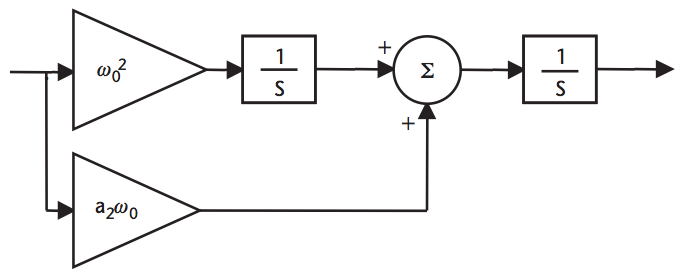
\includegraphics[width=1\textwidth]{Images/LoopArchitectures/SecondOrderLoop.png}
    \caption{Second order loop structure.}
    \label{fig:SecondOrderLoopKaplan}
\end{figure}


\section{State C}
Once the receiver has been in state B for at least 256ms, and if at least 20 of the past 32 measurements have a phase error of less than 30 degrees, then the receiver transitions to state C.

State C has exactly the same loop structure as state B, however the receiver is now considered to be in "phase lock", and data extraction can begin.

\section{State D}

Once the receiver has been in state C for at least 1280ms, the receiver transitions to state D. State D has a 3rd order PLL and a 2nd order FLL.




%Acquisition
%\addcontentsline{toc}{chapter}{Appendix 4}\label{ch:Acquisition}
\chapter{Acquisition}


\begin{figure}[!htb] 
    \centering
    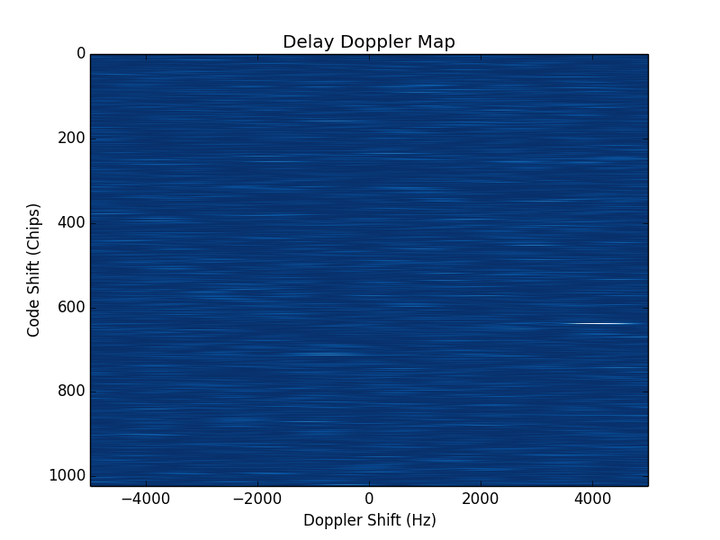
\includegraphics[width=1\textwidth]{Acquisition/DelayDopplerMap.png} 
    \caption{}
    \label{fig:DelayDopplerMap}
\end{figure}

\begin{figure}[!htb] 
    \centering
    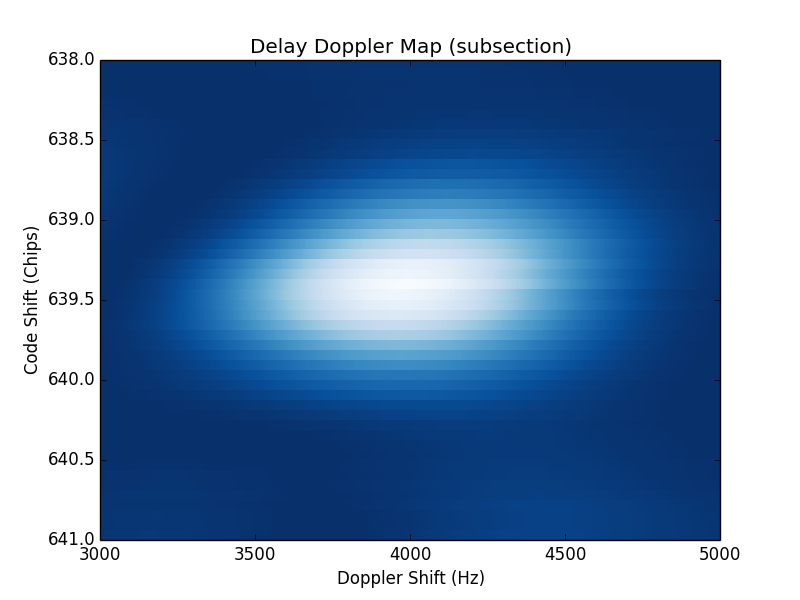
\includegraphics[width=1\textwidth]{Acquisition/DelayDopplerMapSubsection.png} 
    \caption{}
    \label{fig:DelayDopplerMapSubsection}
\end{figure}

%Falcon 9
%\addcontentsline{toc}{chapter}{Appendix 5}\label{ch:Falcon9}
\chapter{Falcon 9 v1.1 flight performance}

In order to develop relevant solutions to  problems in industry, it is important to have an understanding of what the real world challenges faced by the receiver are. A thorough understanding of the real world challenges allows accurate simulations analysis to be carried out.

\begin{figure}[!htb] 
    \centering
    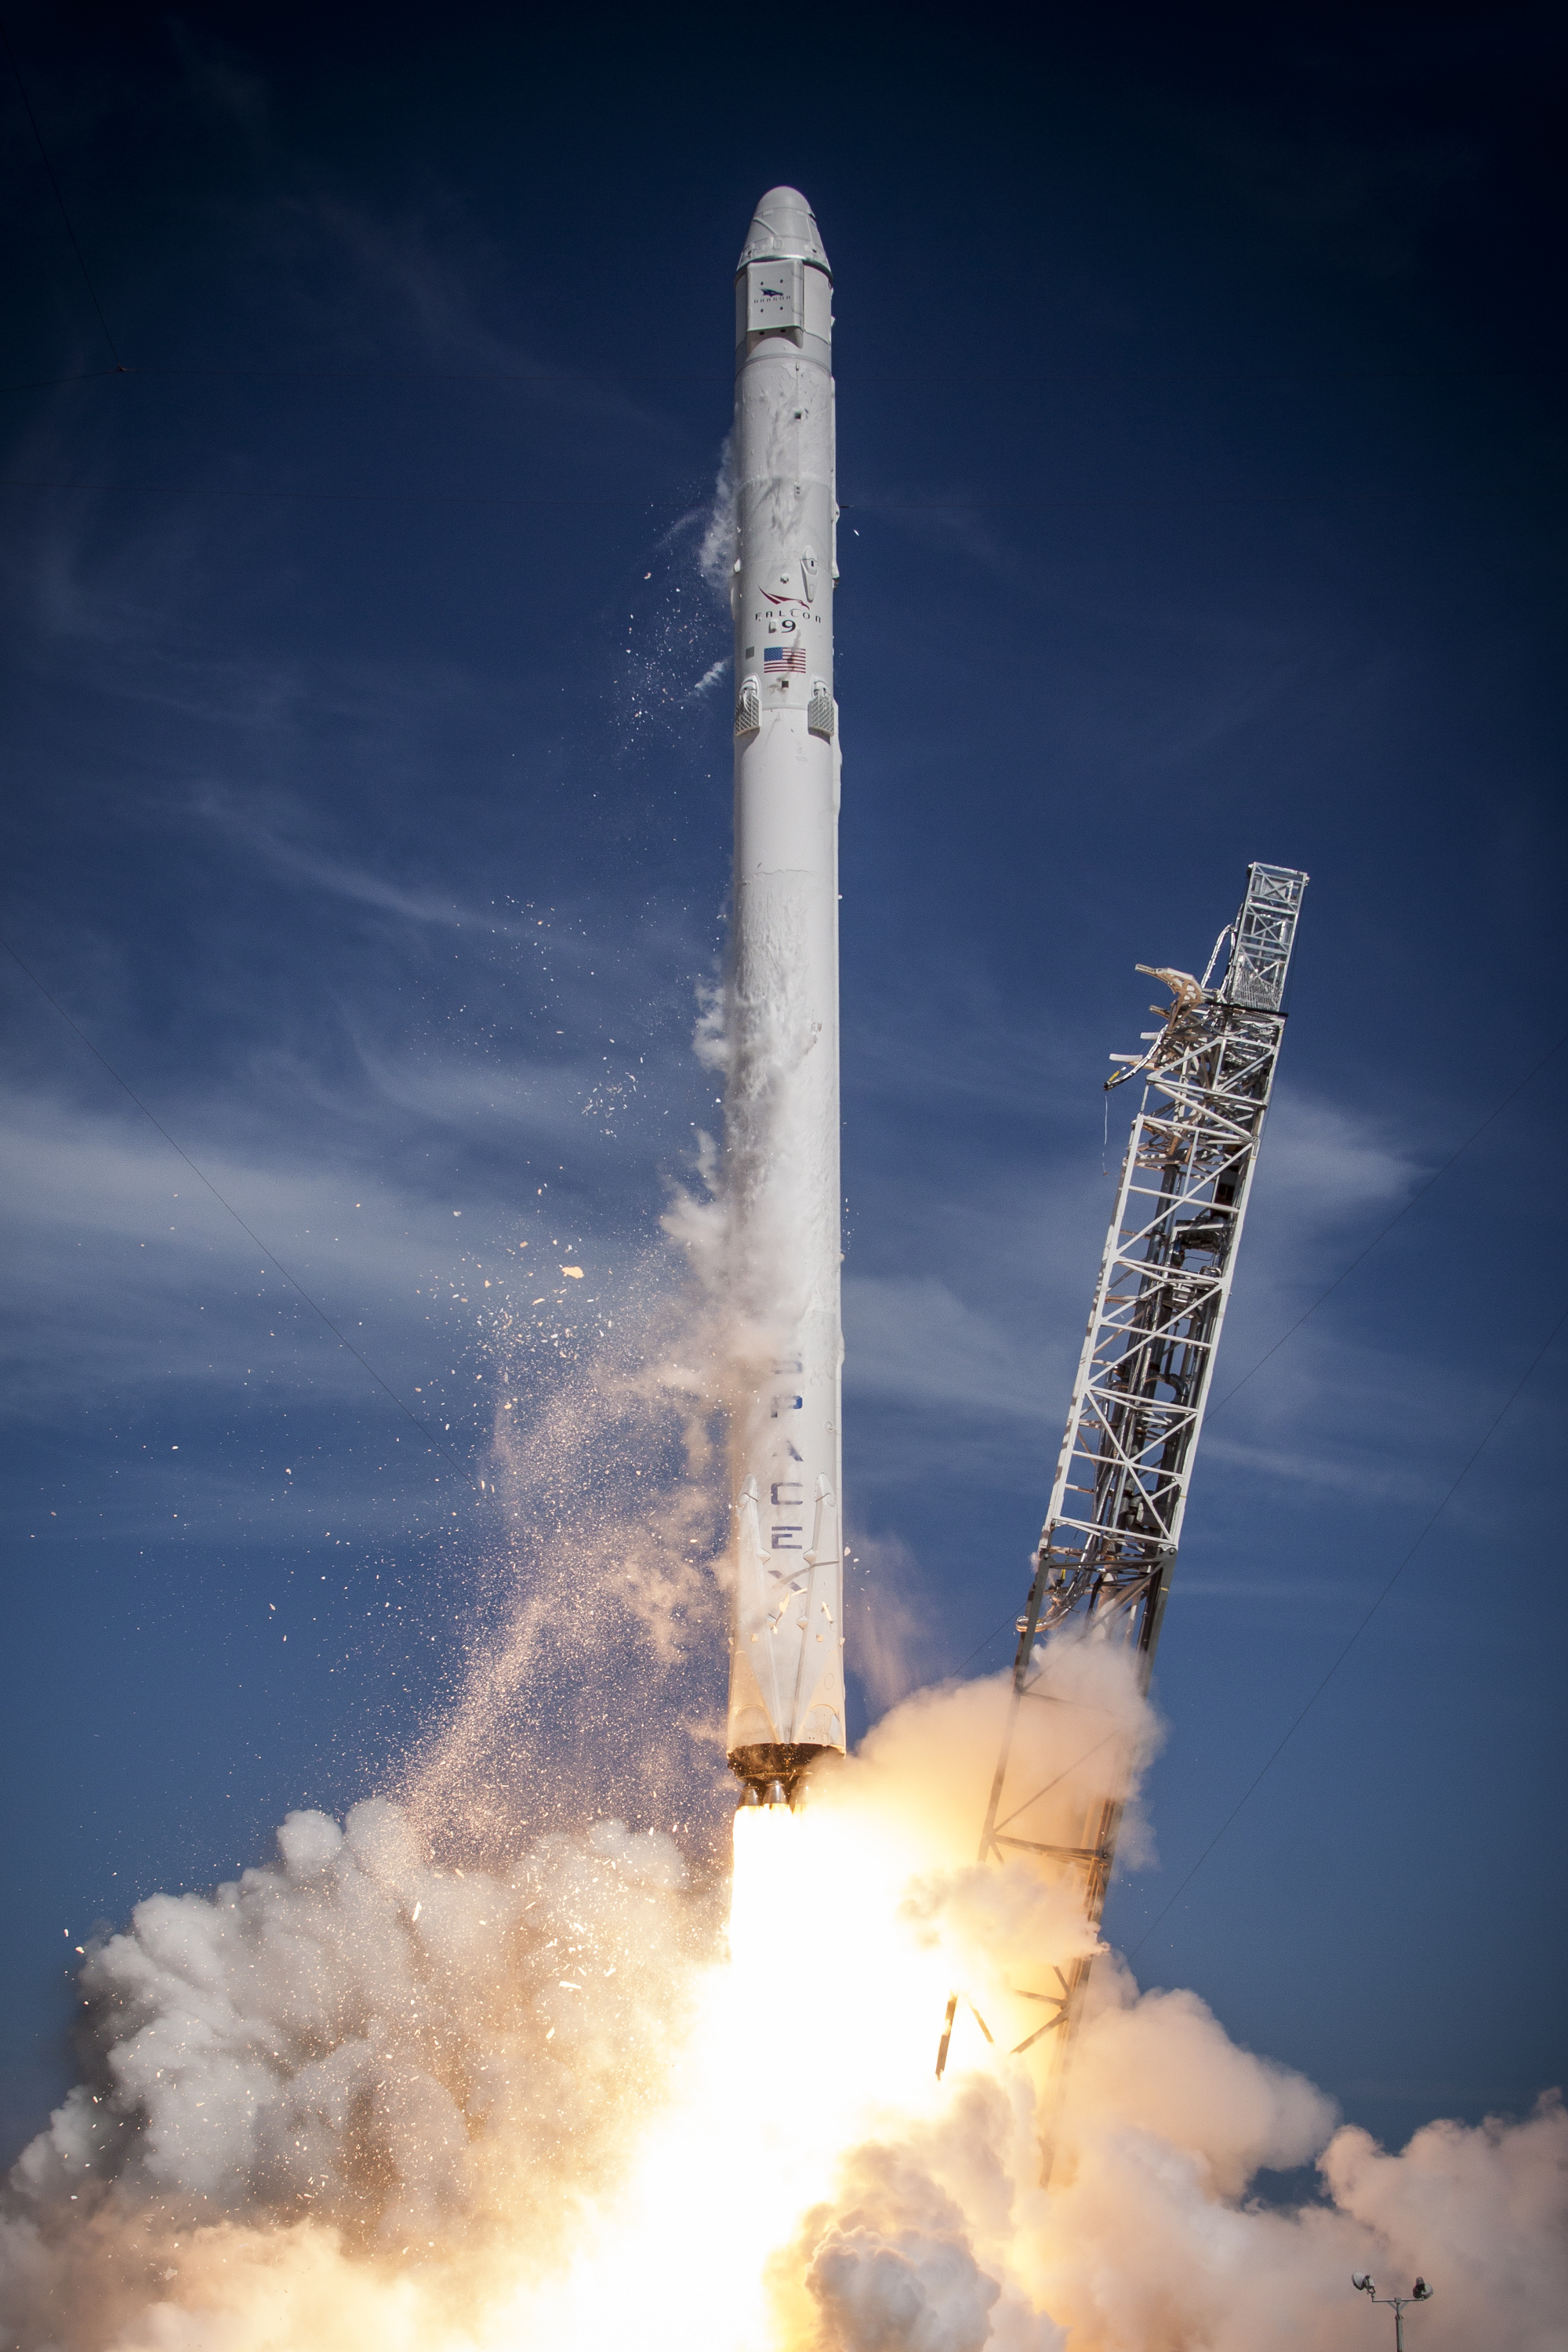
\includegraphics[width=0.9\textwidth]{Falcon9/crs6_launch_center.jpg} 
    \caption{CRS-6 Launch, Image from \cite{SpaceXPhotos}}
    \label{fig:Falcon9}
\end{figure}




In order to meet this goal, the Falcon 9 v1.1 was chosen for analysis. There were a number of reasons for this choice, in particular, the Falcon 9 is gaining industry acceptance, and is likely to represent a significant market share of launches going forward. Additionally, Space Exploration Technology Corporation (SpaceX) who develop,construct and launch the Falcon 9 are more open regarding the technical details of their \ac{LV} than their contemporaries. Finally, the Falcon 9 v1.1 is experiences a wide variety of dynamics, including the first stage conducting a "hover slam" or "suicide burn" manoeuvre, the success of which is reliant on accurate position and velocity estimates.

Because the actual flight performance of the Falcon 9 v1.1 is proprietary and confidential, an effort must be made to develop an model which uses publicly disclosed information. In this manner, a model of the performance can be developed, and compared against real world performance of the \ac{LV}.

\section{Physics model}



\begin{figure}[!htb] 
    \centering
    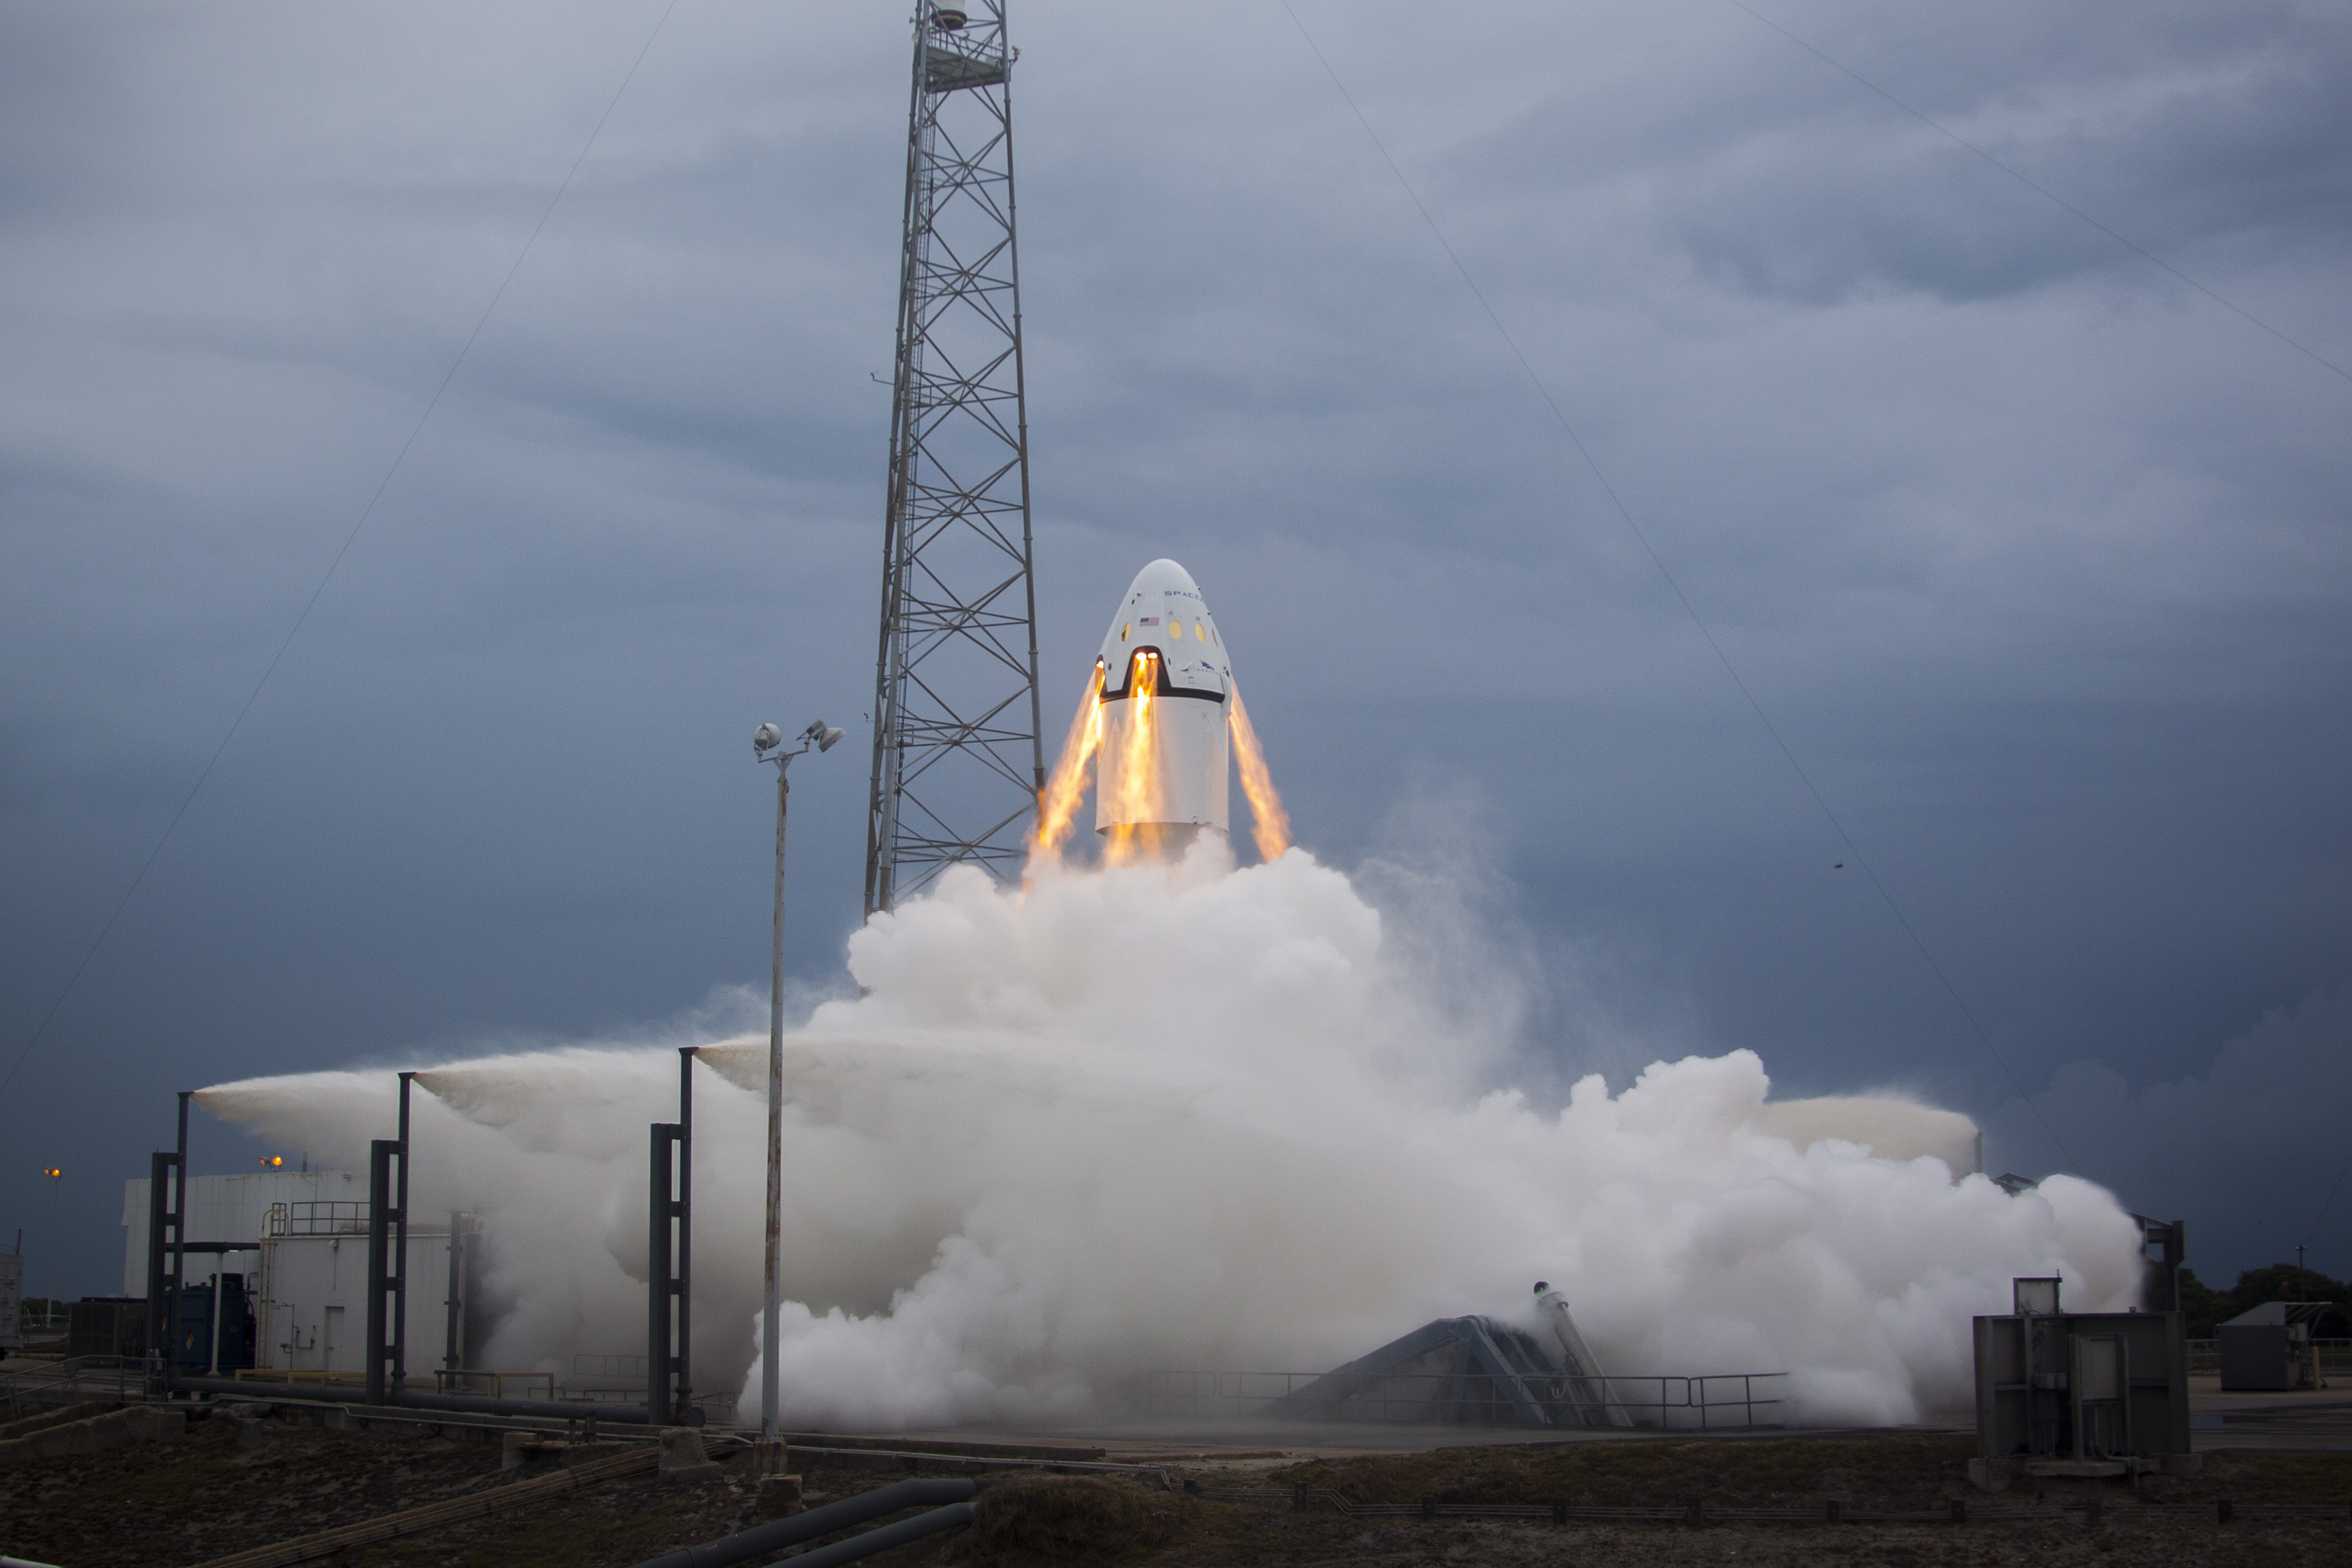
\includegraphics[width=0.9\textwidth]{Falcon9/dragon_pad_abort_launch2.jpg} 
    \caption{Pad abort testing, Image from \cite{SpaceXPhotos}}
    \label{fig:PadAbort}
\end{figure}

\section{Measured performance}

In order to verify the physics model, it must be compared against real world data. Because the true flight performance is proprietary and confidential, the publicly released videos and associated commentary of three different launches were transcribed. 

\begin{table}[!htb]
\centering
\begin{tabular}{|l|l|}
\hline
\rowcolor[HTML]{C0C0C0} 
Time (s) & Event                                \\ \hline
60       & 5.8km alt, 250m/s, 0.8km down range  \\ \hline
\rowcolor[HTML]{EFEFEF} 
86       & Max Q                                \\ \hline
127      & 38km alt, 1160m/s, 19km down range   \\ \hline
\rowcolor[HTML]{EFEFEF} 
150      & 61km alt, 1900m/s, 40km down range   \\ \hline
169      & Stage 1 separation                   \\ \hline
\rowcolor[HTML]{EFEFEF} 
180      & 93km alt, 2120m/s, 79km down range   \\ \hline
265      & 156km alt, 2500m/s, 193km down range \\ \hline
\rowcolor[HTML]{EFEFEF} 
380     & 202km alt, 3700m/s, 420km down range \\ \hline
454      & 210km alt, 4700m/s, 610km down range \\ \hline
\rowcolor[HTML]{EFEFEF} 
540      & 207km alt, 6700m/s, 925km down range \\ \hline
\end{tabular}
\caption{CRS-4 Flight transcript \cite{CRS4}}
\label{tab:CRS4}
\end{table}

\begin{table}[!htb]
\centering
\begin{tabular}{|l|l|}
\hline
\rowcolor[HTML]{C0C0C0} 
Time (s) & Event                                \\ \hline
60       & 5.5km alt, 250m/s 0.9km down range   \\ \hline
\rowcolor[HTML]{EFEFEF} 
97       & Max Q                                \\ \hline
126      & 35km alt, 1000m/s 14.5 km down range \\ \hline
\rowcolor[HTML]{EFEFEF} 
150      & 58km alt, 1800m/s 33 km down range   \\ \hline
165      & Stage 1 seperation                   \\ \hline
\rowcolor[HTML]{EFEFEF} 
185      & 90km alt, 1900m/s 67km down range    \\ \hline
240      & 134km alt, 2100m/s, 135km down range \\ \hline
\rowcolor[HTML]{EFEFEF} 
270      & Stage 1 boost-back start             \\ \hline
300      & 166km alt, 2600m/s                   \\ \hline
\rowcolor[HTML]{EFEFEF} 
316      & Stage 1 boost-back stop              \\ \hline
412      & Stage 1 entry burn start             \\ \hline
\rowcolor[HTML]{EFEFEF} 
428      & Stage 1 entry burn stop              \\ \hline
435      & 205km alt, 4200km, (garbled) down range    \\ \hline
\rowcolor[HTML]{EFEFEF} 
475      & Stage 1 transonic                    \\ \hline
514      & Stage 1 under horizon                \\ \hline
\rowcolor[HTML]{EFEFEF} 
540      & 208km, 6900m/s 850km down range      \\ \hline
565      & Stage 2 engine shutdown              \\ \hline
\end{tabular}
\caption{CRS-5 Flight transcript \cite{CRS5}}
\label{tab:CRS5}
\end{table}

\begin{table}[!htb]
\centering
\begin{tabular}{|l|l|}
\hline
\rowcolor[HTML]{C0C0C0} 
Time (s) & Event                                 \\ \hline
120      & 32km alt, 1000m/s, 13.5km down range  \\ \hline
\rowcolor[HTML]{EFEFEF} 
165      & Stage seperation                      \\ \hline
180      & 86km alt, 1950m/s, 63km down range    \\ \hline
\rowcolor[HTML]{EFEFEF} 
277      & Stage 1 boost-back start              \\ \hline
300      & 165km alt, 2560m/s, 212km down range  \\ \hline
\rowcolor[HTML]{EFEFEF} 
315      & Stage 1 boost-back stop               \\ \hline
405      & Stage 1 entry burn start              \\ \hline
\rowcolor[HTML]{EFEFEF} 
425      & Stage 1 entry burn stop               \\ \hline
450      & 205km alt, 4400m/s, 530km down range  \\ \hline
\rowcolor[HTML]{EFEFEF} 
491      & Stage 1 transonic                     \\ \hline
540      & 208 km alt, 6500m/s, 830km down range \\ \hline
\rowcolor[HTML]{EFEFEF} 
574      & Stage 2 shutdown \\ \hline
\end{tabular}
\caption{CRS-6 Flight transcript \cite{CRS6}}
\label{tab:CRS6}
\end{table}



\begin{figure}[!htb]
\centering

\includegraphics[scale=1]{Falcon9/Falcon9R.pdf}
\caption{Falcon 9 Rocket}
\label{fig:Rocket}
\end{figure}

\section{Velocity Requirements}
The 2nd stage burn must be terminated at precisely the right time, to ensure that the final velocity is correct. This is because the orbital height is dictated by the velocity, 

\begin{equation}
v_0 = \sqrt{\frac{G \cdot M}{r}}
\end{equation}

Where:
\begin{align*}
G &= 6.673 \times 10^{-11} N m^2 kg^{-2}\\
M &= 5.972 \times 10^{24} kg
\end{align*}

\begin{equation}
r = \frac{G \cdot M}{v_0^2}
\end{equation}

\begin{equation}
\frac{dr}{dv} = \frac{-2 \cdot G \cdot M}{v_0^3}
\end{equation}

For \ac{LEO}, with an orbital velocity of $\approx$ 7,800 m/s, this results in a a differential of 1,679m of altitude, per m/s of velocity. Given that SpaceX guarantees orbital height of $\pm$ 10km, this results in a velocity tolerance of $\pm$ 5.95 m/s, or $\pm$ 31.2 Hz of doppler shift.


\begin{table}[!htb]
\centering
\begin{tabular}{|l|l|l|l|l|l|}
\hline
\rowcolor[HTML]{C0C0C0} 
Date      & Vehicle       & No    & Payload      & Mass (Tons)         & Orbit                  \\ \hline
21/9/2014 & Falcon 9 v1.1 & F9-13 & CRS-4 Dragon & $\approx$ 9.3  & 199x359x51.64  LEO/ISS \\ \hline
\rowcolor[HTML]{EFEFEF} 
10/1/2015 & Falcon 9 v1.1 & F9-14 & CRS-5 Dragon & $\approx$ 9.54 & 206x353x51.6 LEO/ISS   \\ \hline
14/5/2015 & Falcon 9 v1.1 & F9-18 & CRS-6 Dragon & $\approx$ 9.24 & 199x364x51.65  LEO/ISS \\ \hline
\end{tabular}
\caption{My caption}
\label{FOOBAR}
\end{table}
\cite{Falcon9Stats}


\begin{table}[!htb]
\centering
\begin{tabular}{|l|l|}
\hline
\rowcolor[HTML]{C0C0C0} 
Time (s) & Event                                     \\ \hline
0.0      & Liftoff from Cape Canaveral               \\ \hline
\rowcolor[HTML]{EFEFEF} 
7.5      & Initial Pitch Kick                        \\ \hline
55.0     & Begin gravity turn                        \\ \hline
\rowcolor[HTML]{EFEFEF} 
76.0     & Max-Q                                     \\ \hline
115.0    & Release angle of attack restrictions      \\ \hline
\rowcolor[HTML]{EFEFEF} 
155.5    & Shutdown 2 engines for acceleration limit \\ \hline
174.2    & Main Engine Cut Off                       \\ \hline
\rowcolor[HTML]{EFEFEF} 
176.2    & Stage 1/Stage 2 separation                \\ \hline
179.2    & Second stage engine start \#1             \\ \hline
\rowcolor[HTML]{EFEFEF} 
199.2    & Payload fairing jettison                  \\ \hline
475.9    & Second stage engine cut off               \\ \hline
\end{tabular}
\caption{Falcon 9 Sample Flight Time-line \cite{Falcon9}}
\label{tab:Falcon9Timeline}
\end{table}

\begin{figure}[!htb] 
    \centering
    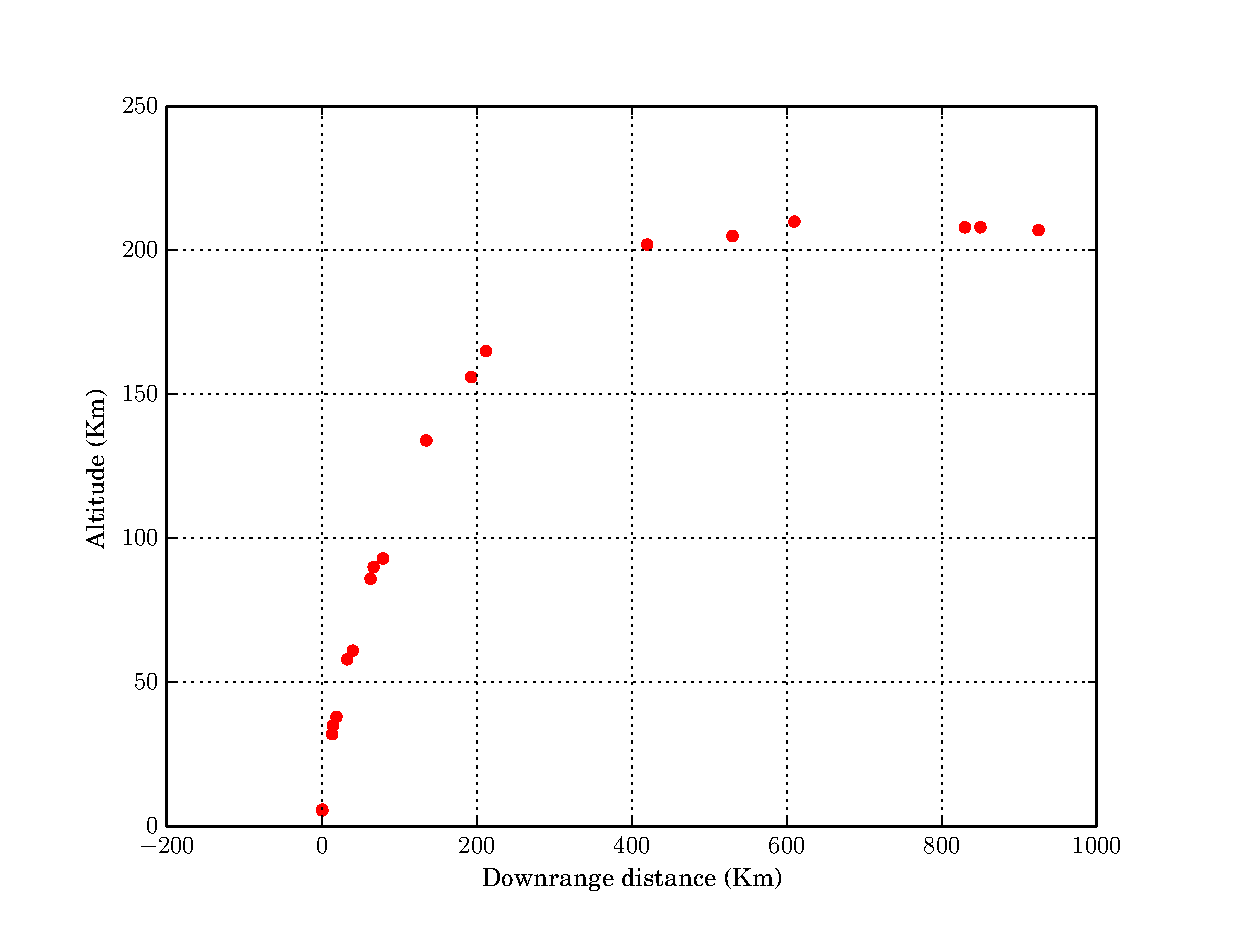
\includegraphics[width=1\textwidth]{Falcon9/FlightProfile.eps} 
    \caption{The Falcon 9 V1.1 flight profile, compare with figure \ref{fig:Falcon9Launch}.}
    \label{fig:Faclon9FlightProfile}
\end{figure}


\begin{figure}[!htb] 
    \centering
    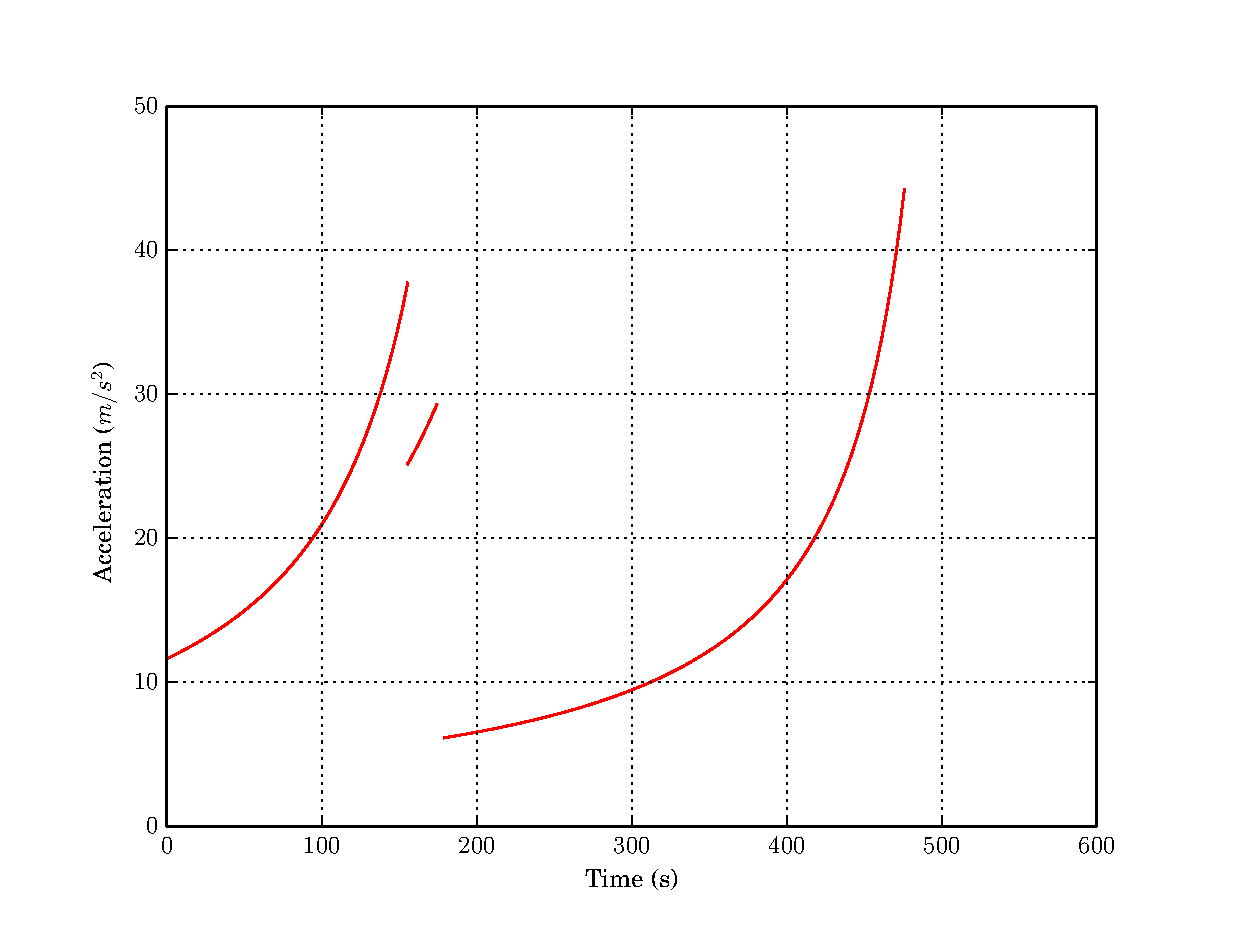
\includegraphics[width=1\textwidth]{Falcon9/Model.eps}
    \caption{}
    \label{fig:Falcon9Model}
\end{figure}


\begin{figure}[!htb] 
    \centering
    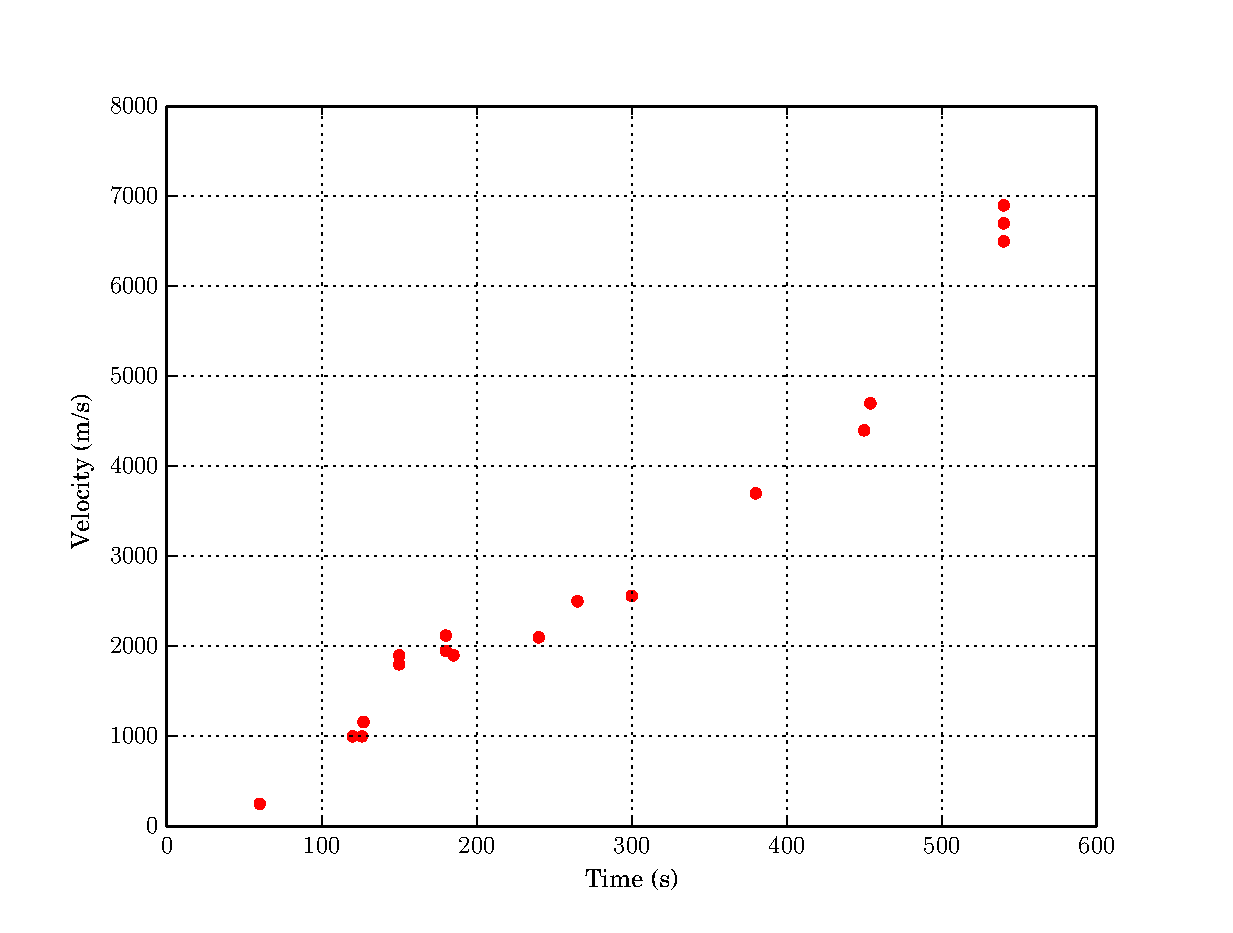
\includegraphics[width=1\textwidth]{Falcon9/VelocityProfile.eps}
    \caption{}
    \label{fig:Falcon9VelocityProfile}
\end{figure}



\begin{figure}[!htb] 
    \centering
    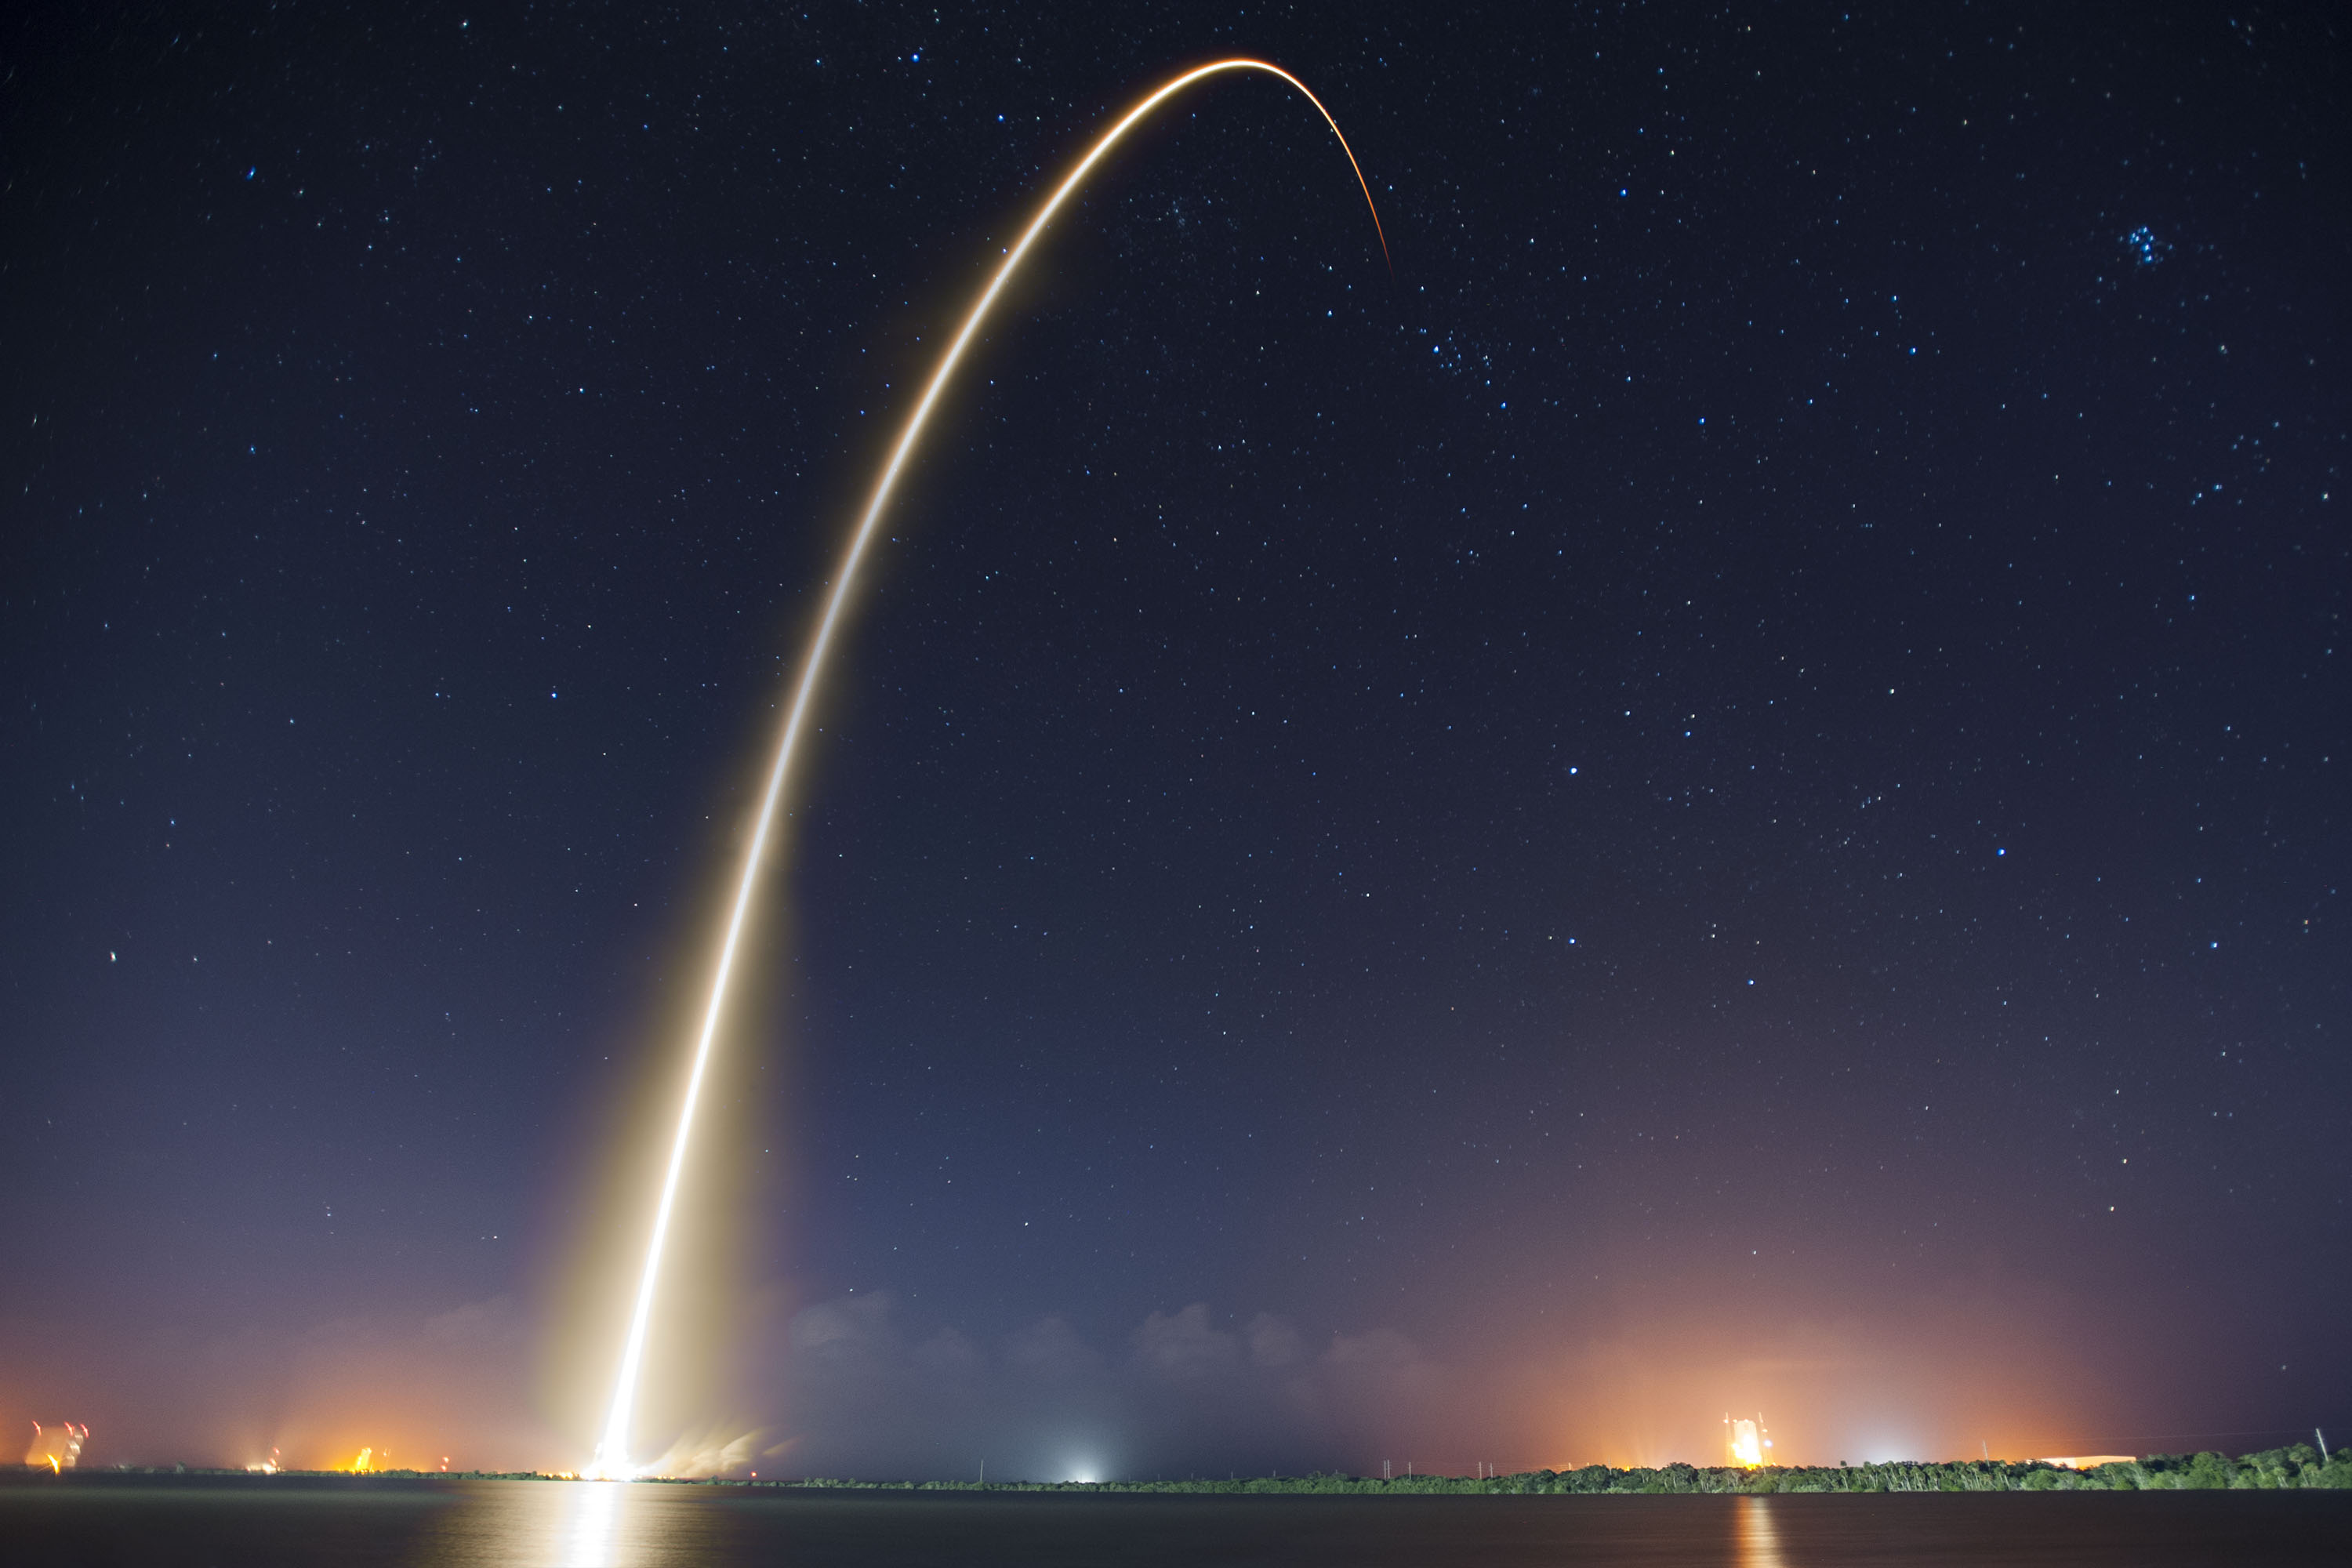
\includegraphics[width=1\textwidth]{Falcon9/Launch1.jpg}
    \caption{An oblique view of a Falcon 9 V1.1 launch. \cite{SpaceXFalcon9}}
    \label{fig:Falcon9Launch}
\end{figure}


\section{Launch Azimuth}

\begin{equation}
\beta = arcsin \Big(\frac{cos(i)}{cos(\phi)}\Big)
\end{equation}

Where:
\begin{align*}
 i &= \text{Orbit inclination}\\
 \phi &= \text{Launch site latitude}\\
 \beta &= \text{Launch azimuth}\\
\end{align*}

\cite{LaunchDesign}

The \ac{ISS} has an inclination of $51.6\degree$, hence a launch from Cape Canaveral ($\phi = 28.5\degree$), $\beta=44.9\degree$.


\begin{figure}[!htb] 
    \centering
    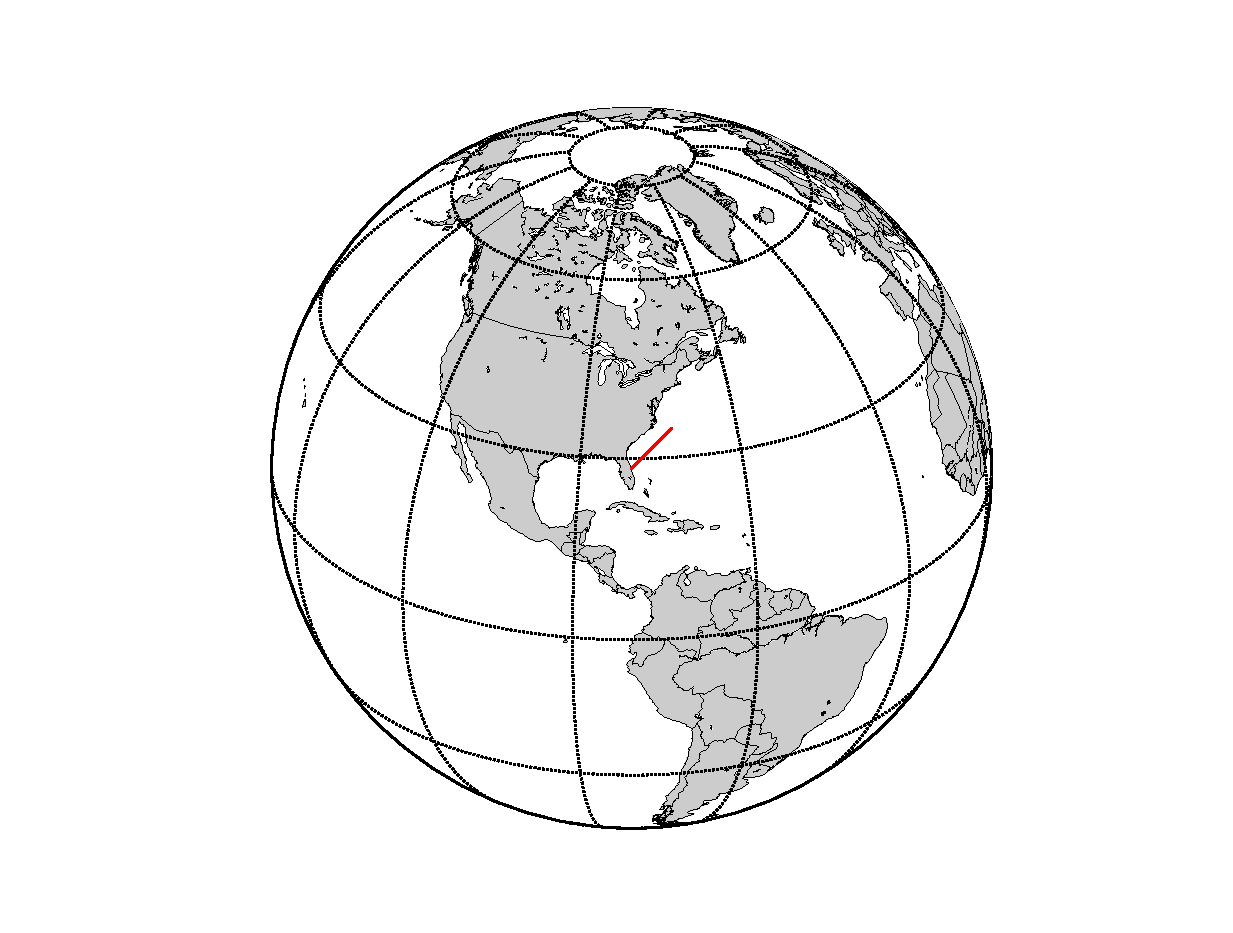
\includegraphics[width=1\textwidth]{Falcon9/CapeCanaveral.eps}
    \caption{}
    \label{fig:LaunchPath}
\end{figure}




\begin{figure}[!htb] 
    \centering
    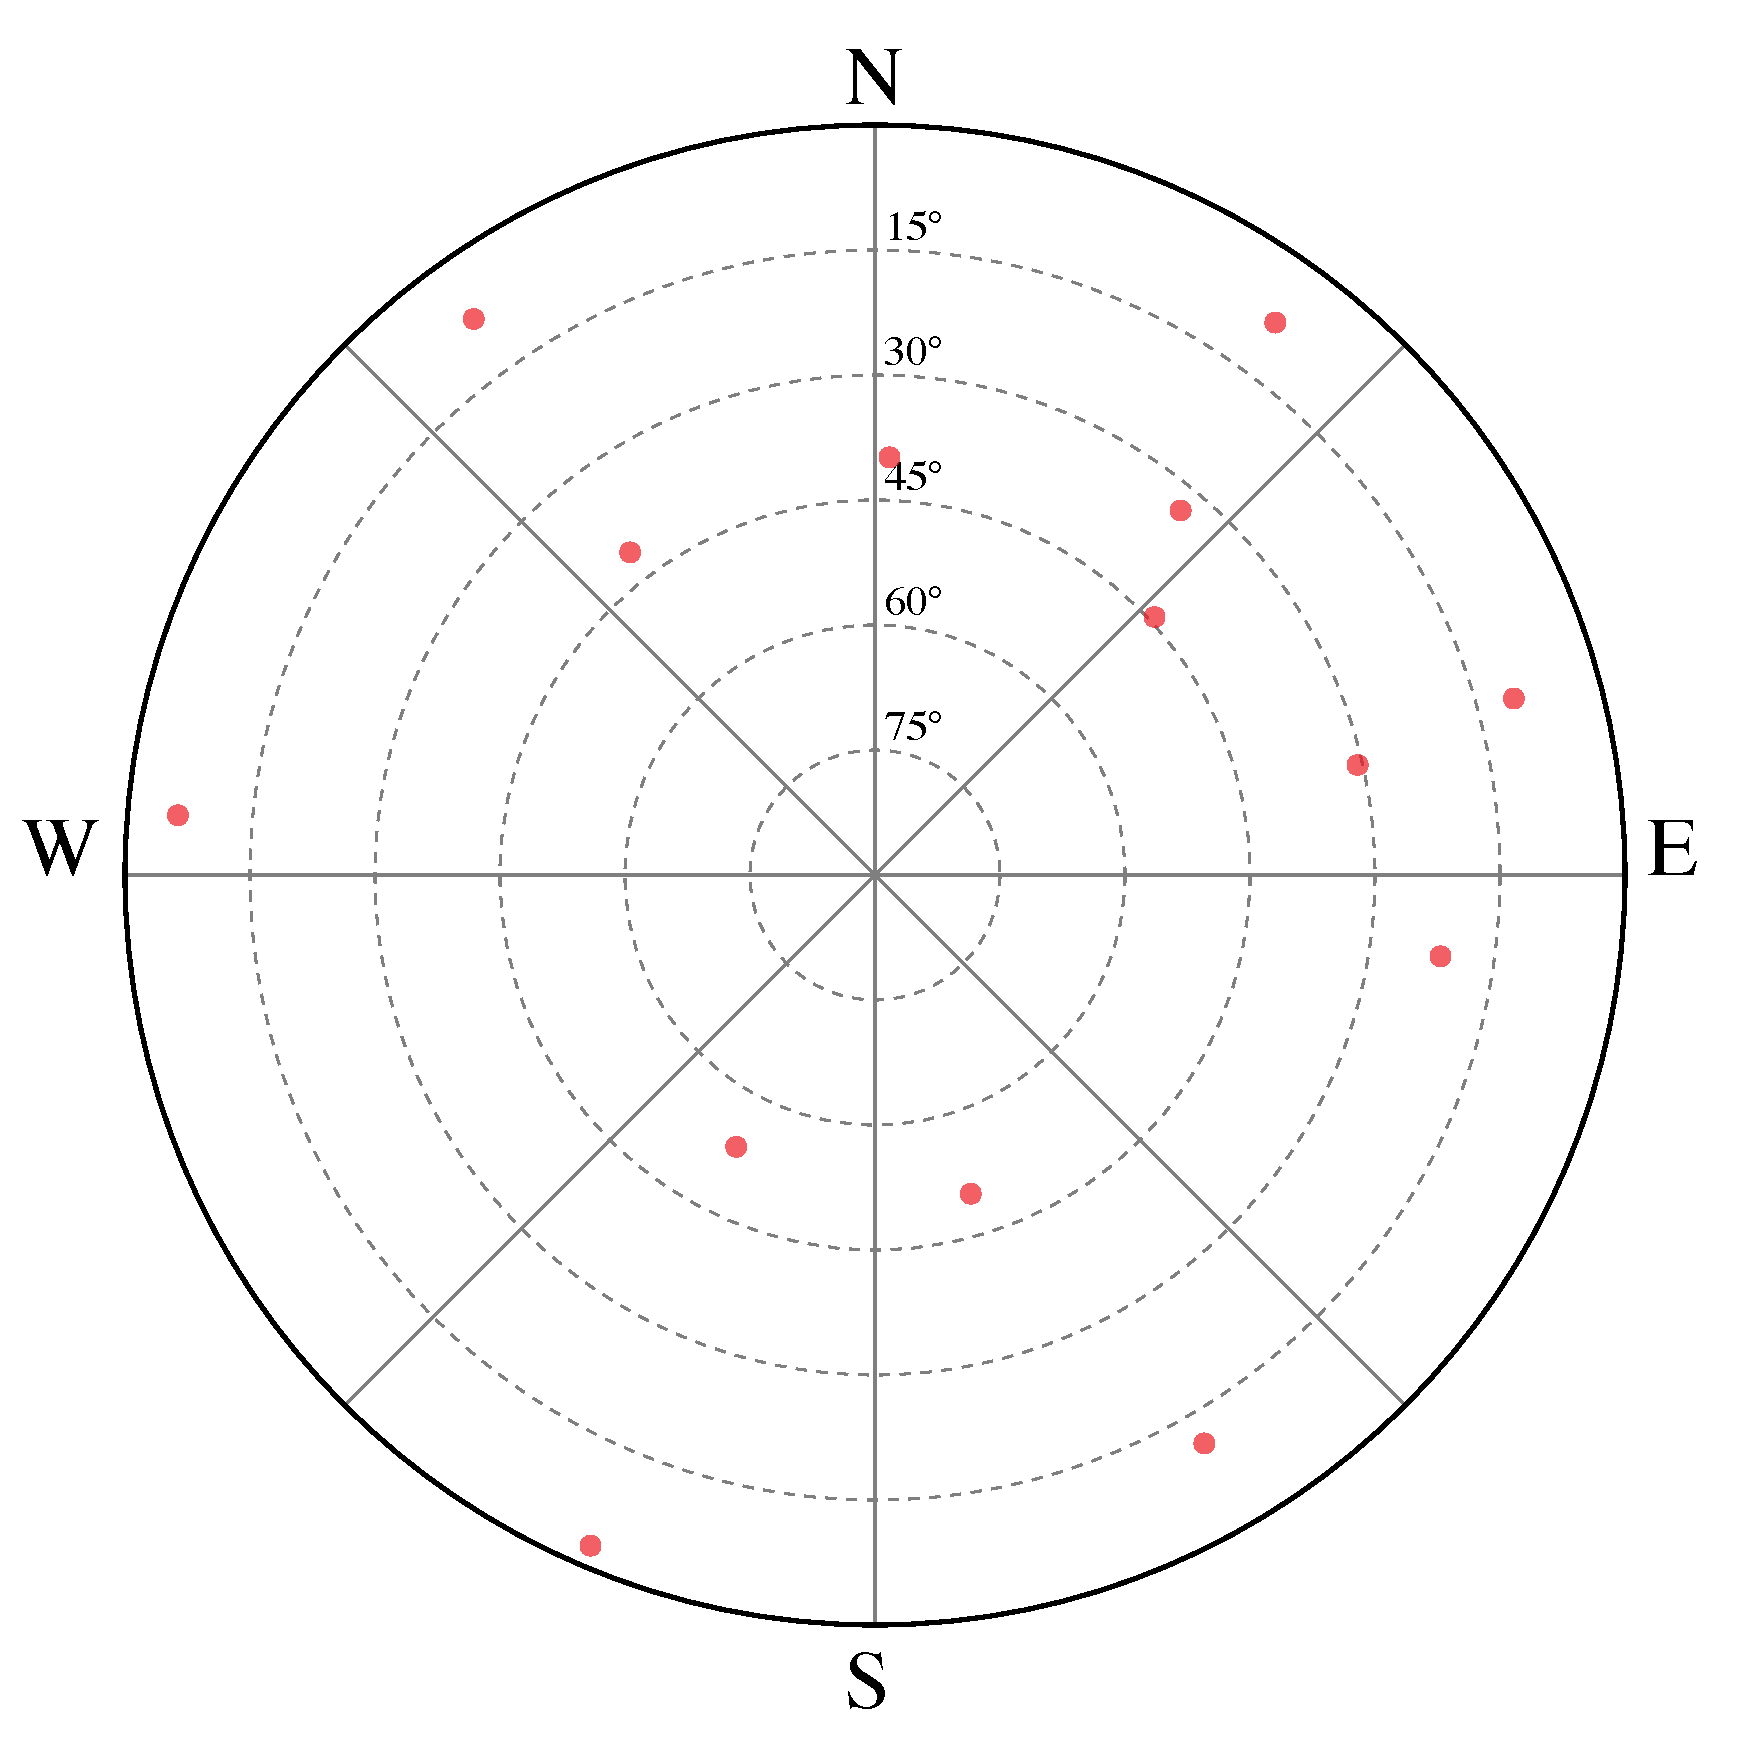
\includegraphics[width=1\textwidth]{Falcon9/Skyplot.pdf}
    \caption{}
    \label{fig:Skyplot}
\end{figure}





%Discriminators and Sampling
%\addcontentsline{toc}{chapter}{Appendix 6}\label{app6}
\chapter{Discriminators \& Sampling}

The role of the discriminator is to determine the error (frequency or phase), based on current an previous I \& Q samples. This is computed every second incoherent dump (8ms), because a pair of samples is required to compute frequency. 

The Discriminator for both the FLL and PLL loops comes from Kaplan, and can be found on pages (Insert pages here).


\tikzset{
block/.style = {draw, fill=white, rectangle, minimum height=3em, minimum width=3em},
tmp/.style  = {coordinate}, 
sum/.style= {draw, fill=white, circle, node distance=1cm},
input/.style = {coordinate},
output/.style= {coordinate},
pinstyle/.style = {pin edge={to-,thin,black}
}
}

\begin{figure}[!htb]
\centering
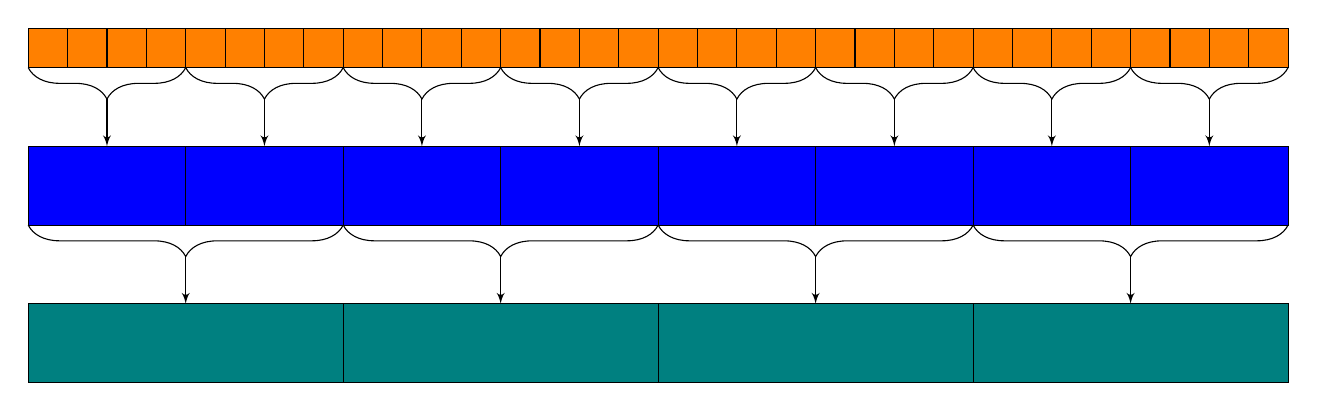
\begin{tikzpicture}[auto, node distance=2cm,>=latex']

%\draw[dotted](-3,0.25) node {Coherent samples};
%\draw[dotted](-3,-1.5) node {Incoherent integration};
%\draw[dotted](-3,-3.5) node {Frequencies};

    

\foreach \x in {0,...,31}{
    \draw [fill=orange] (0.5*\x,0) rectangle (0.5*\x+0.5,0.5);
}

\foreach \x in {0,...,7}{
    \draw [fill=blue] (2*\x,-1) rectangle (2*\x+2,-2);
}

\foreach \x in {0,...,3}{
    \draw [fill=teal] (4*\x,-3) rectangle (4*\x+4,-4);
}

\foreach \x in {0,...,7}{
\draw [decorate,decoration={brace,amplitude=0.4cm,mirror},xshift=0,yshift=0pt]
(2*\x,0) -- (2*\x+2,0) node [black,midway]{};
}

\foreach \x in {0,...,7}{
    \draw[->] (2*\x+1,-0.4) -- (2*\x+1,-1);
}

\foreach \x in {0,...,3}{
    \draw [decorate,decoration={brace,amplitude=0.4cm,mirror},xshift=0,yshift=0pt]
(4*\x,-2) -- (4*\x+4,-2) node [black,midway]{};
}

\foreach \x in {0,...,3}{
    \draw[->] (4*\x+2,-2.4) -- (4*\x+2,-3);
}

\end{tikzpicture}
\caption{An overview of the sampling process.1 ms long coherently integrated samples (orange)  are produced by the hardware correlator.Four of these are coherently integrated together to generate the inputs to the tracking loop (blue). The FLL and PLL discriminator both take a pair of 4ms long samples to produce an estimate of the phase/frequency (teal).}
\label{fig:SamplingSchemeA}
\end{figure}






\tikzset{
block/.style = {draw, fill=white, rectangle, minimum height=3em, minimum width=3em},
tmp/.style  = {coordinate}, 
sum/.style= {draw, fill=white, circle, node distance=1cm},
input/.style = {coordinate},
output/.style= {coordinate},
pinstyle/.style = {pin edge={to-,thin,black}
}
}

\begin{figure}[!htb]
\centering
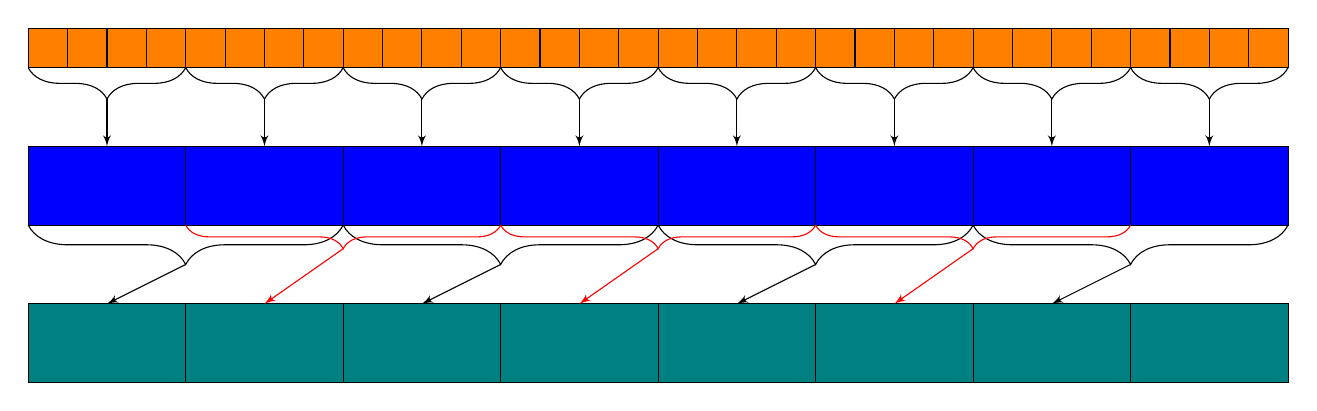
\begin{tikzpicture}[auto, node distance=2cm,>=latex']

%\draw[dotted](-3,0.25) node {Coherent samples};
%\draw[dotted](-3,-1.5) node {Incoherent integration};
%\draw[dotted](-3,-3.5) node {Frequencies};

\foreach \x in {0,...,31}{
    \draw [fill=orange] (0.5*\x,0) rectangle (0.5*\x+0.5,0.5);
}

\foreach \x in {0,...,7}{
    \draw [fill=blue] (2*\x,-1) rectangle (2*\x+2,-2);
}


\foreach \x in {0,...,7}{
    \draw [fill=teal] (2*\x,-3) rectangle (2*\x+2,-4);
}


\foreach \x in {0,...,7}{
    \draw [decorate,decoration={brace,amplitude=0.4cm,mirror},xshift=0,yshift=0pt]
(2*\x,0) -- (2*\x+2,0) node [black,midway]{};
    \draw[->] (2*\x+1,-0.4) -- (2*\x+1,-1);
}


\foreach \x in {0,...,3}{
    \draw [decorate,decoration={brace,amplitude=0.5cm,mirror},xshift=0,yshift=0pt]
(4*\x,-2) -- (4*\x+4,-2) node [black,midway]{};
    \draw[->] (4*\x+2,-2.5) -- (4*\x+1,-3);
}

\foreach \x in {0,...,2}{
    \draw [red,decorate,decoration={brace,amplitude=0.3cm,mirror},xshift=0,yshift=0pt]
(4*\x+2,-2) -- (4*\x+6,-2) node [black,midway]{};
    \draw[->,red] (4*\x+4,-2.3) -- (4*\x+3,-3);
}

\end{tikzpicture}
\caption{As compared to the sampling process outlined in figure \ref{fig:SamplingSchemeA}, this scheme provides frequency and phase estimates every 4ms.}
\label{fig:SamplingB}
\end{figure}






\tikzset{
block/.style = {draw, fill=white, rectangle, minimum height=3em, minimum width=3em},
tmp/.style  = {coordinate}, 
sum/.style= {draw, fill=white, circle, node distance=1cm},
input/.style = {coordinate},
output/.style= {coordinate},
pinstyle/.style = {pin edge={to-,thin,black}
}
}

\begin{figure}[!htb]
\centering
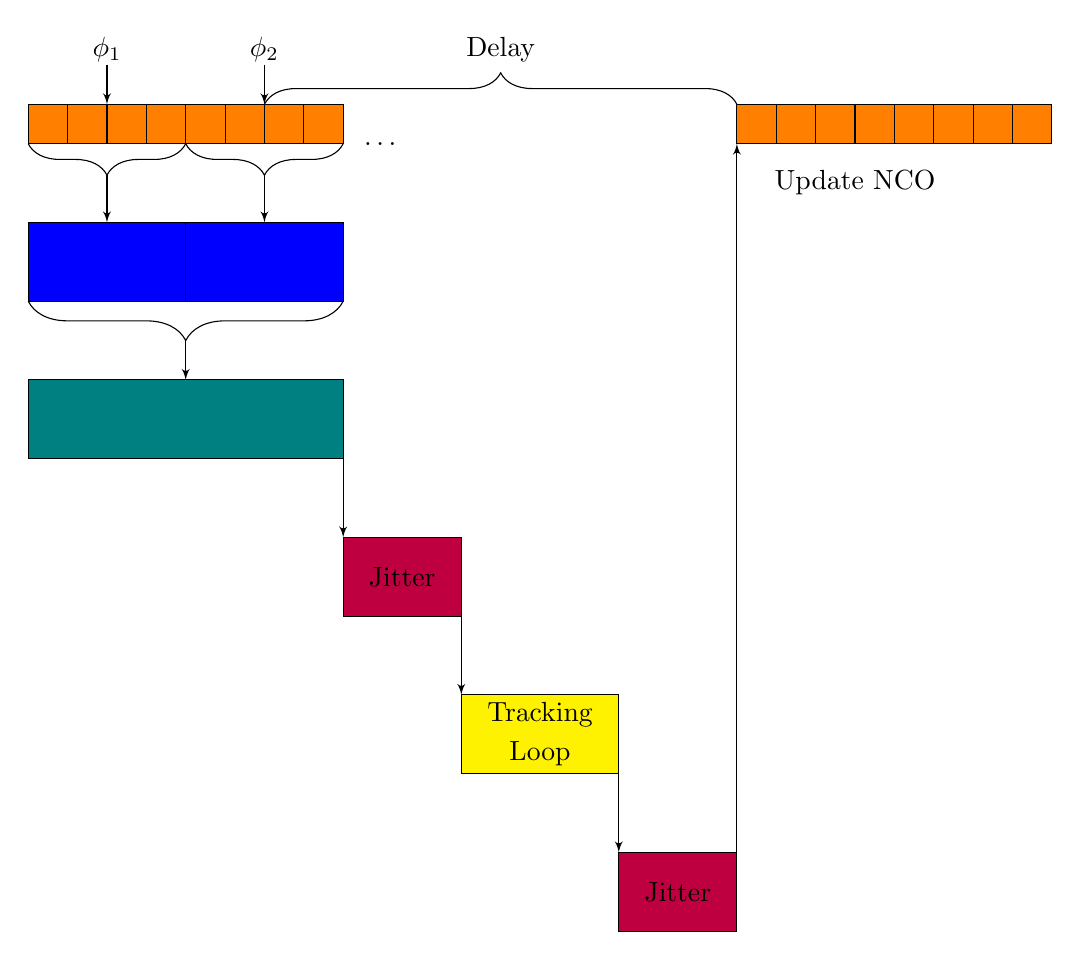
\begin{tikzpicture}[auto, node distance=2cm,>=latex']

%\draw[dotted](-3,0.25) node {Coherent samples};
%\draw[dotted](-3,-1.5) node {Incoherent integration};
%\draw[dotted](-3,-3.5) node {Frequencies};


\draw[->] (1,1) -- (1,0.5);
\draw[->] (3,1) -- (3,0.5);
\node at (1,1.2) {$\phi_1$};
\node at (3,1.2) {$\phi_2$};


\foreach \x in {0,...,7}{
    \draw [fill=orange] (0.5*\x,0) rectangle (0.5*\x+0.5,0.5);
}


\foreach \x in {0,...,7}{
    \draw [fill=orange] (0.5*\x+9,0) rectangle (0.5*\x+0.5+9,0.5);
}


\node at (4.5,0) {\ldots};


\foreach \x in {0,...,1}{
    \draw [fill=blue] (2*\x,-1) rectangle (2*\x+2,-2);
}

\draw [fill=teal] (0,-3) rectangle (4,-4);


\foreach \x in {0,...,1}{
    \draw [decorate,decoration={brace,amplitude=0.4cm,mirror},xshift=0,yshift=0pt]
(2*\x,0) -- (2*\x+2,0) node [black,midway]{};
    \draw[->] (2*\x+1,-0.4) -- (2*\x+1,-1);
}


\draw [decorate,decoration={brace,amplitude=0.5cm,mirror},xshift=0,yshift=0pt]
(0,-2) -- (4,-2) node [black,midway]{};
\draw[->] (2,-2.5) -- (2,-3);


\draw[->] (4,-4) -- (4,-5);
\draw [fill=purple] (4,-5) rectangle (5.5,-6);
\node at (4.75,-5.5) {Jitter};


\draw[->] (5.5,-6) -- (5.5,-7);
\draw [fill=yellow] (5.5,-7) rectangle (7.5,-8);
\node at (6.5,-7.25) {Tracking};
\node at (6.5,-7.75) {Loop};


\draw[->] (7.5,-8) -- (7.5,-9);
\draw [fill=purple] (7.5,-9) rectangle (9,-10);
\node at (8.25,-9.5) {Jitter};

\draw[->] (9,-9) -- (9,0);
\node at (10.5,-0.5) {Update NCO};


\draw [decorate,decoration={brace,amplitude=0.4cm},xshift=0,yshift=0pt]
(3,0.5) -- (9,0.5) node [black,midway]{};

%\draw[->] (9,1.5) -- (9,0.5);
\node at (6,1.2) {Delay};


\end{tikzpicture}
\caption{Once a pair of 4ms coherently integrated samples has been collected, then the tracking loops can compute a new value for the NCO. During this process, delays accrue due to the interrupt driven nature of the processor, as well as processing time for the tracking loops.}
\label{fig:SamplingJitter}
\end{figure}






\begin{comment}
"It is important to note that the timing of each of the correlator channels will be locked to its own incoming signal and not to each other or to the microprocessor interrupts, so new data is generated asynchronously. The sampling instant of measurement data of all channels however is common to give a consistent navigation solution."

"Carrier DCO Programming
The following registers: CHx_CARRIER_DCO_INCR_HIGH (or X_DCO _INCR_HIGH) and CHx_CARRIER_DCO_INCR_LOW
are programmed in sequence with the relevant data according to the frequency bin being searched. It is always necessary to write to both the _HIGH and _LOW registers. Carrier DCO programming will become effective as soon as the channel is released (made active). If the channel is already active, writes to CHx_CARRIER_DCO_INCR_LOW are effective immediately. (A short delay of up to 175ns will occur, to allow synchronisation of the processor write operation to the chip operation.)"
\cite{GP2021}
\end{comment}

\subsection{Arctangent}
The arctangent function is used in the discriminators for both the FLL and the PLL. It is important to note that there are two different types of arctangent function, the 
\lstinputlisting[language=Python,frame=single]{Code/ATan2.py}

Some additional logic is included in the function to ensure that the function always returns a value, even when X is equal to zero.

\begin{figure}[!htb] 
    \centering
    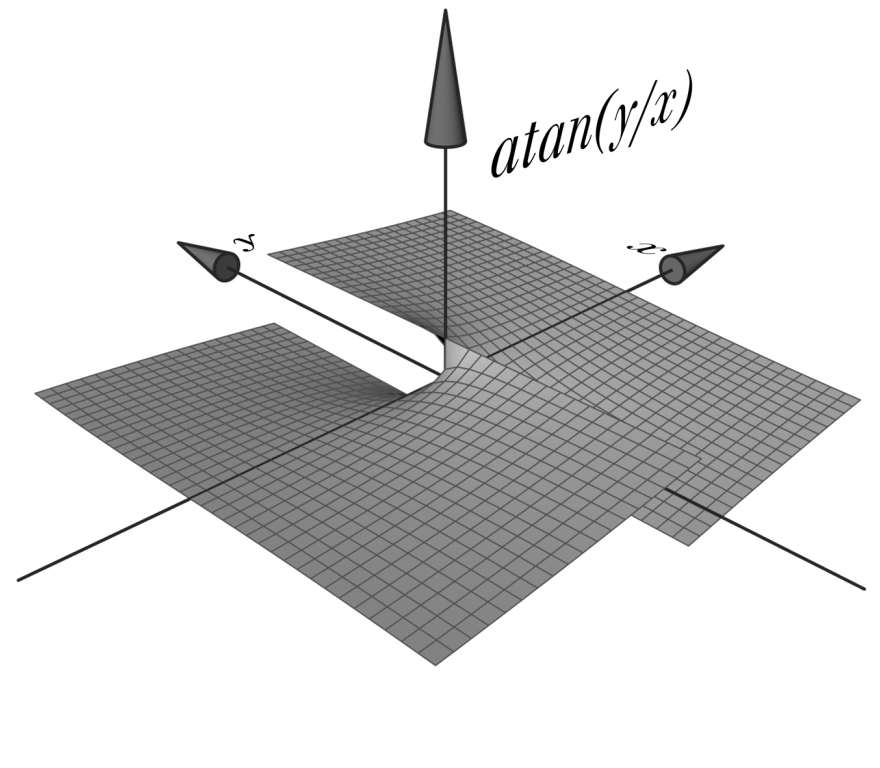
\includegraphics[width=1\textwidth]{Discriminators/ATanDiagram.png} 
    \caption{}
    \label{fig:ATanDiagram}
\end{figure}

\begin{figure}[!htb] 
    \centering
    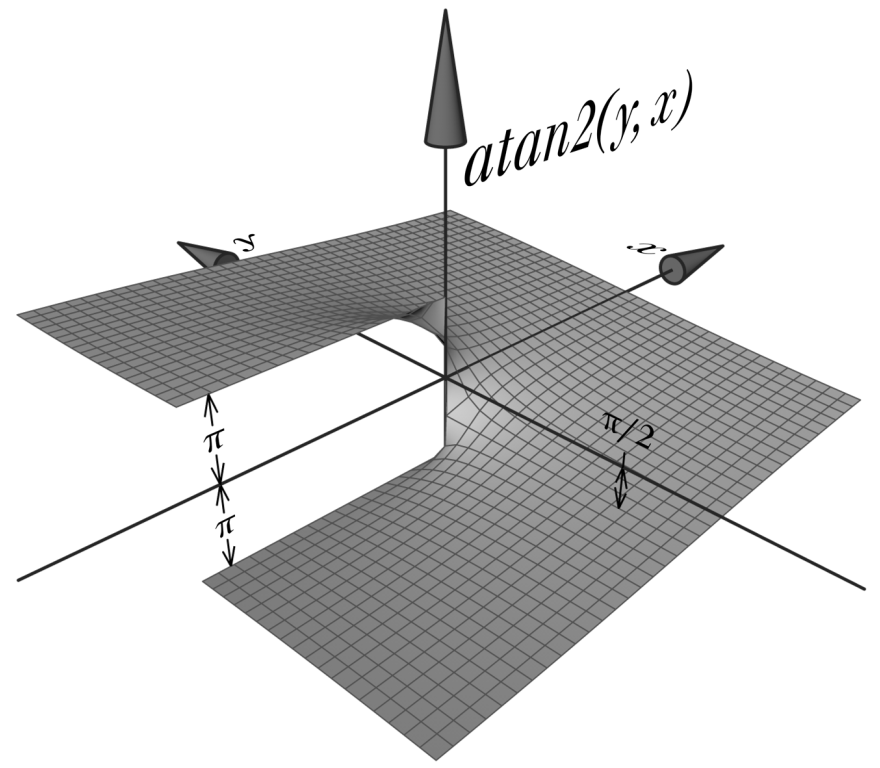
\includegraphics[width=1\textwidth]{Discriminators/ATan2Diagram.png} 
    \caption{}
    \label{fig:ATan2Diagram}
\end{figure}


\subsection{FLL Discriminator}
The role of the FLL discriminator is to convert pairs of phase measurements into frequency. A key statistic for the FLL discriminator is it's capture range. This can be computed as 
$\frac{-1}{2T} < f < \frac{1}{2T}$
, where $T = 0.004$

Hence the FLL has a locking range of $\pm 125Hz$. 

If the frequency of the incoming signal is outside this range, then a false lock will occur due to aliasing. This can be seen in figure(Insert picture of aliasing). 

The FLL discriminator which is described in Kaplan uses the dot and cross product of the previous two samples.
$$Dot = I_{k}\times I_{k-1} + Q_{k}\times Q_{k-1}$$
$$Cross = Q_{k} \times I_{k-1} - I_{k} \times K_{k-1}$$
$$DeltaPhase = ATan2(Cross,Dot)$$

\begin{figure}[!htb] 
    \centering
    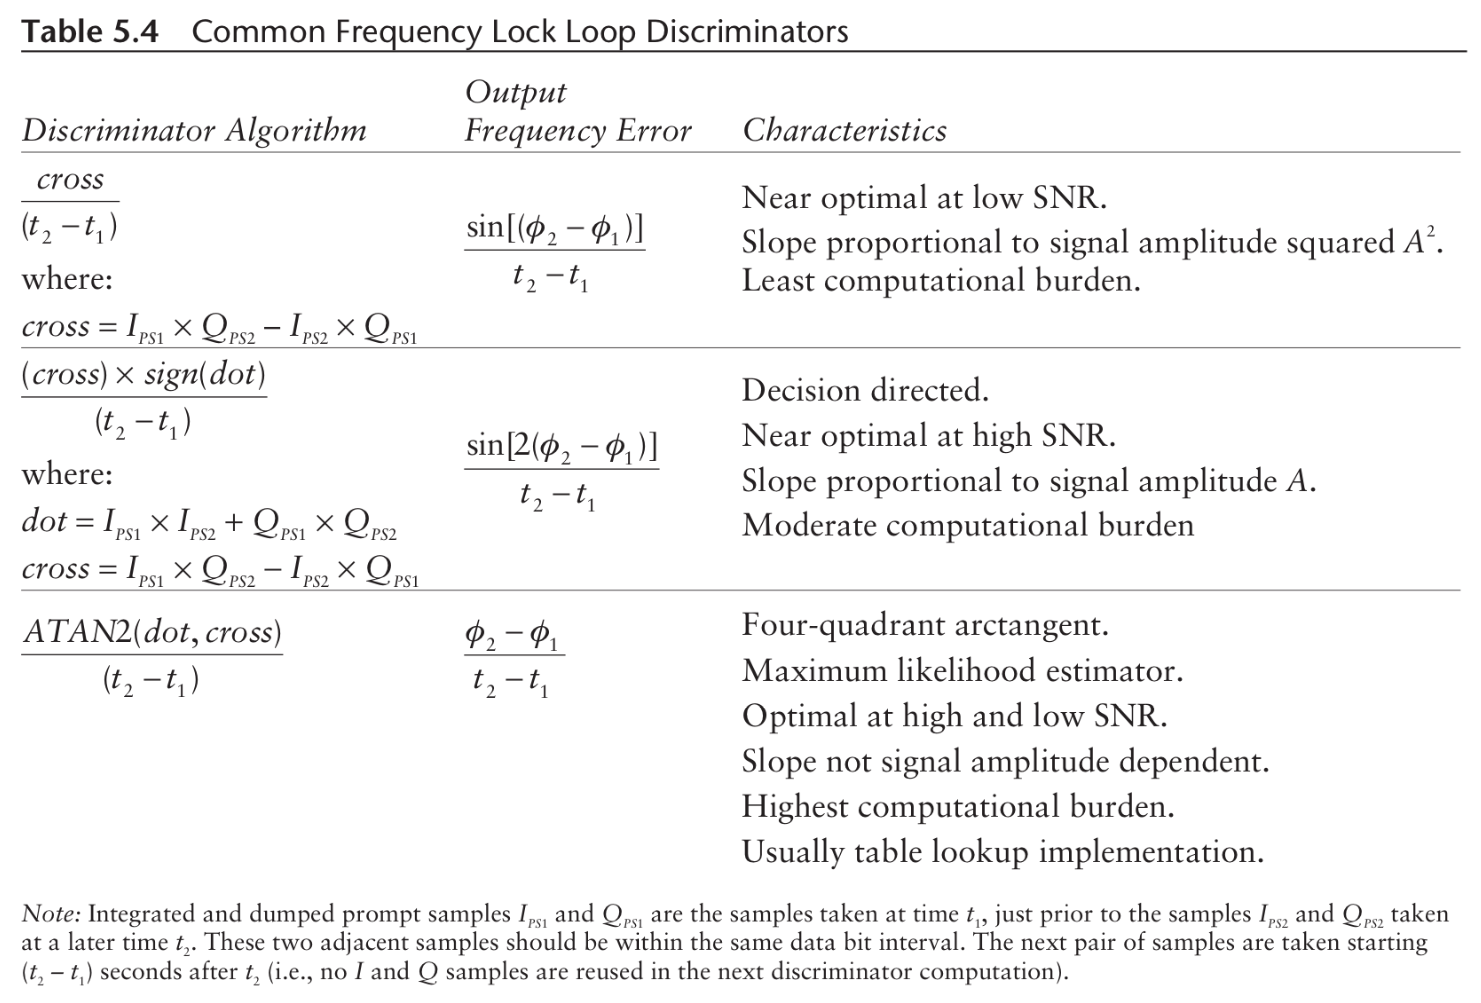
\includegraphics[width=1\textwidth]{Discriminators/FLLDiscriminator.png} 
    \caption{The different FLL discriminators presented in Kaplan.\cite{Kaplan}}
    \label{fig:FLLDiscriminatorTable}
\end{figure}


\lstinputlisting[language=Python,frame=single]{Code/FLLDiscriminator.py}

\subsection{PLL Discriminator}
The goal of the PLL Discriminator is to determine the current phase error. In the case of the current implementation, computed phase 


\begin{figure}[!htb] 
    \centering
    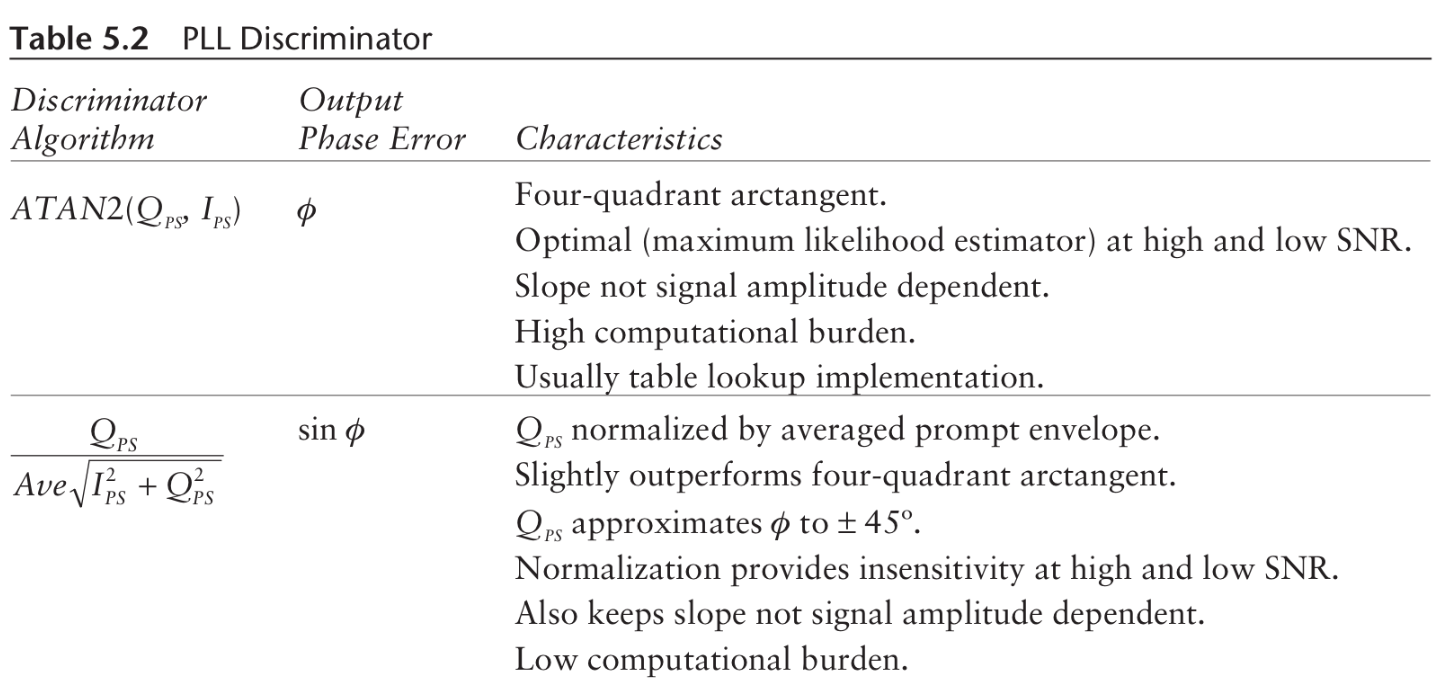
\includegraphics[width=1\textwidth]{Discriminators/PLLDiscriminator.png} 
    \caption{The different PLL discriminators presented in Kaplan.\cite{Kaplan}}
    \label{fig:PLLDiscriminatorTable}
\end{figure}

\begin{figure}[!htb] 
    \centering
    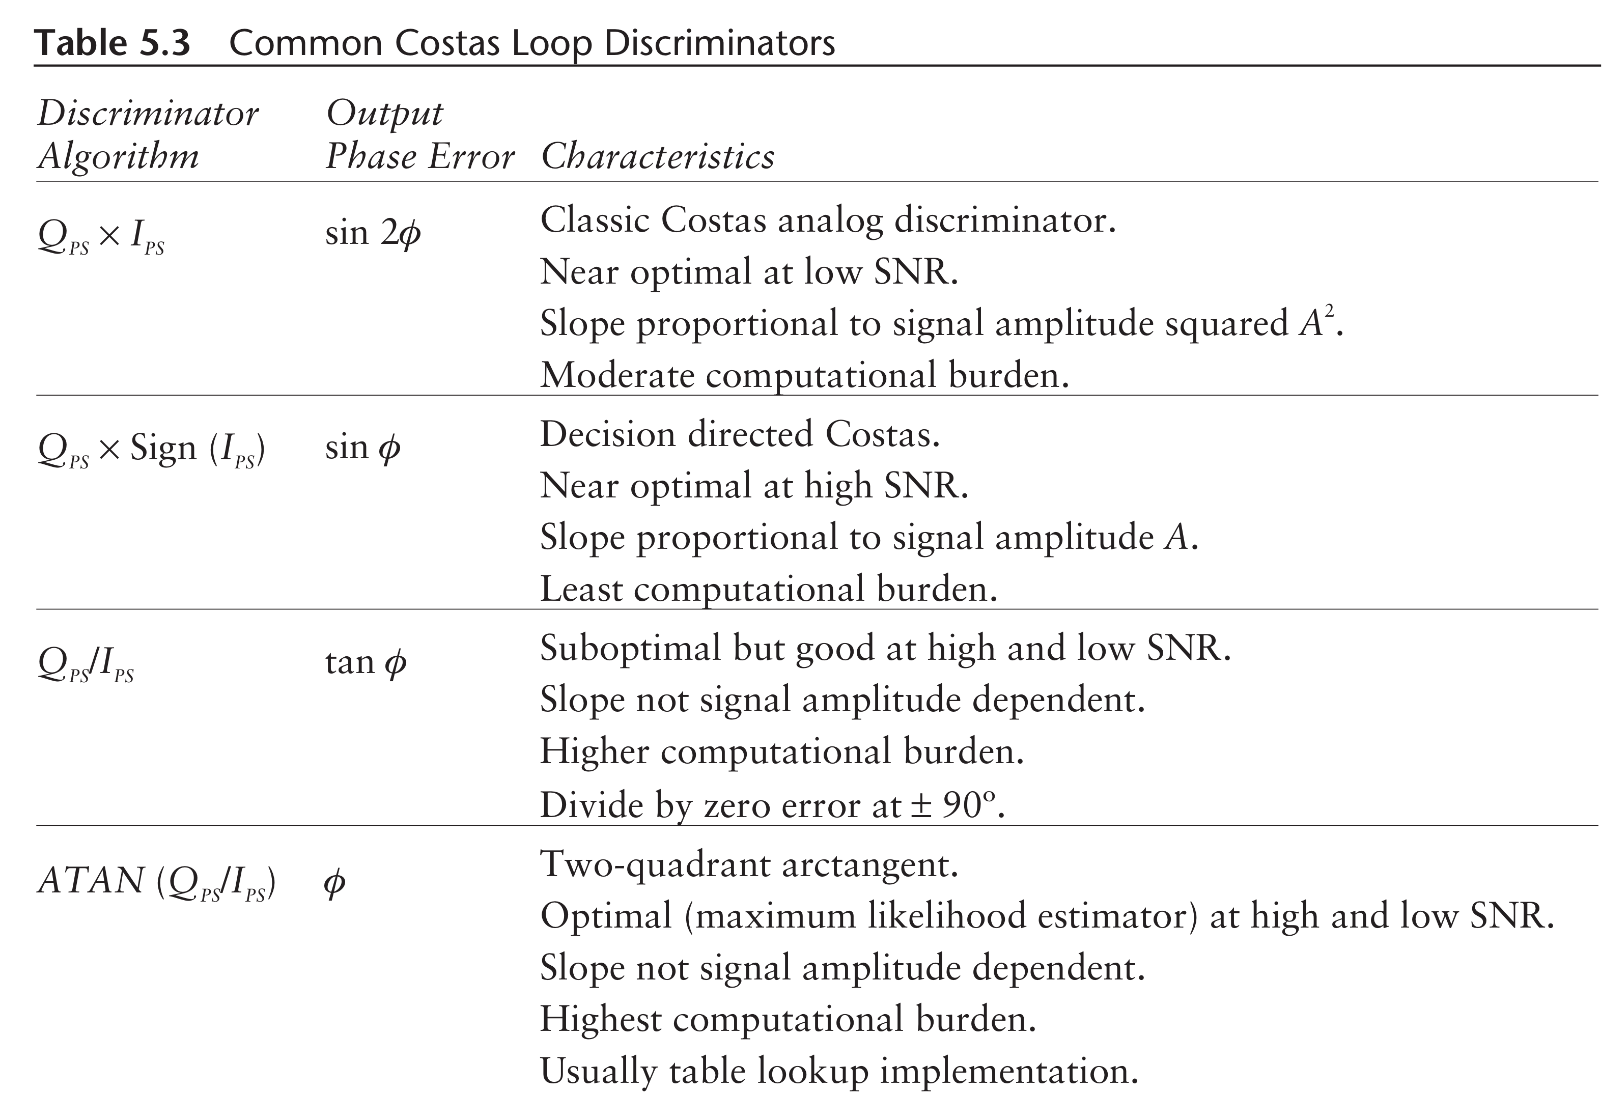
\includegraphics[width=1\textwidth]{Discriminators/CostasDiscriminator.png} 
    \caption{The different Costas loop discriminators presented in Kaplan.\cite{Kaplan}}
    \label{fig:CostasDiscriminatorTable}
\end{figure}

$Z_{k} \times \overline{Z_{k-1}}$

%\lstinputlisting[language=Python,frame=single]{Code/PLLDiscriminator.py}

%Code
%\addcontentsline{toc}{chapter}{Appendix 7}\label{app7}
\chapter{Code}

\subsection{Receiver.py}
\lstinputlisting[language=Python]{Code/Receiver.py}

\subsection{TrackingLoop.py}
\lstinputlisting[language=Python]{Code/TrackingLoop.py}

\subsection{GenSignal.py}
\lstinputlisting[language=Python]{Code/GenSignal.py}


%Vibration
%\addcontentsline{toc}{chapter}{Appendix 8}\label{ch:Vibrations}
\chapter{Vibrations}


\begin{comment}
"Vibration is not just a rocket issue, though. All electronic hardware is tested for its ability to handle shock and vibration. An MP3 player, for example, has to be tested for its ability to handle the vibrations from someone walking or jogging while holding it, placing it on a counter top, or accidentally dropping it on the floor. However, compared to the workout that Ares I-X’s avionics receive, your MP3 player has got it easy. Imagine shaking that MP3 player inside an automatic paint can shaker for two minutes while continuing to play your favourite tunes. That’s kind of what the electronics of the I-X are up against."
\end{comment}

\emph{"Imagine shaking that MP3 player inside an automatic paint can shaker for two minutes while continuing to play your favourite tunes. That's kind of what the electronics are up against."} \cite{MITRocketVibrations}

As discussed before, dynamics can affect the \ac{GNSS} receiver in two fundamental ways. Low frequency dynamics (\ac{QSL}) result in the receiver accelerating, and the nominal carrier frequency changing due to the doppler shift. 

Dynamics can also affect the receiver by placing mechanical loads upon the quartz crystal used as a frequency reference in the receiver. From the receiver's perspective, a change in the carrier frequency is indistinguishable from a change in the local oscillator frequency generated by the quartz crystal\cite{Kaplan}. 

\subsection{Crystals}
Understanding the impact of vibrations on the crystal is vital for understanding the performance that can be expected from the receiver during ascent \& re-entry. While the receivers ability to deal with dynamics can be assessed readily in the laboratory using a GPS simulator, assessing the impact of vibrations on the receiver is somewhat more complex.

While all mechanical stresses on the crystal cause changes in the frequency produced, for analysis purposes, they are typically grouped in into two categories, namely acceleration stresses, and vibration stresses. 

\begin{comment}
http://www.vectron.com/products/g_sensitivity/Vig-tutorial%20on%20g-sensitivity.pdf
\end{comment}

The  Kea receiver uses the Abracon ASVTX-12 \ac{TCXO}\cite{ASTX12Datasheet}, while the flight model Biarri uses the Vectron  VT-803 TCXO\cite{VT803Datasheet}. While information on g sensitivity is not published for either of these \ac{TCXO}, 
Kaplan suggests that a typical value for g sensitivity is $1 ppb/g$ \cite{Kaplan}.

Additionally, much can be discovered from examining the specification of similar models. The TX-705 oscillator is specifically designed for applications where superior g-sensitivity is required. From the data sheet, we can observe that the g sensitivity of the crystal is consistently less than at $0.1ppb/g$ in the range from 20Hz to 2000Hz \cite{TX705Datasheet}. It is reasonable to expect that the performance of the VT-803 and the ASVTX-12 will be somewhat inferior to the TX-705, however the specification provide guidance on the order of magnitude of sensitivity that can be expected.

\subsection{Mitigation}
There are 4 main strategies for mitigation.

\begin{itemize}
\item{Part specification}
\item{Orientation}
\item{Mechanical isolation}
\item{Electrical compensation}
\end{itemize}

"Frequency shift is a function of the magnitude and direction of the
acceleration, and is usually linear with magnitude up to at least 50 g's."
\cite{CrystalVibration}


\subsubsection{Part specification}
\subsubsection{Orientation}
\subsubsection{Mechanical isolation}
\subsubsection{Electrical compensation}

\subsection{Determining g-sensitivity}
There are three main methods for determining the the g-sensitivity of the receiver.

\begin{itemize}
\item{Manufacturers data sheet}
\item{2g Tip over test}
\item{Vibration testing}
\end{itemize}

Manufacturers datasheets are a preferred solution, however the g-sensitivity may not be provided, especially if the \ac{TCXO} is not designed with g-sensitivity in mind. Additionally,  the g-sensitivity of a \ac{TCXO} may be commercial in confidence, with manufacturer unwilling to share the performance of their crystal, especially for a university who is not going to mass produce a design using that part. 

One simple method of determining the g-sensitivity of the crystal is the 2g tip over test. The test is conceptually simple, and is carried out in the following manner:

\begin{enumerate}
\item{Measure the frequency output of the crystal in one orientation}
\item{Rotate the crystal 180 \degree about an axis}
\item{Measure the frequency output again}
\end{enumerate}

 The g-sensitivity can be found as:

\begin{equation}
\frac{f_1-f_2}{2 f_1}\text{ ppb/g}
\end{equation}

A final method is to place the crystal on a vibrating table. 

\begin{comment}
In recent years significant progress has been made in
crystal resonator design to effect a substantial reduction in
g-sensitivity values [1]. With such reduced levels of
acceleration sensitivity, the need has arisen for a
measurement system with appropriately higher resolution.
The most obvious method for determination of g-sensitivity
for a stable ovenized oscillator is the '2g tip over
test', where the whole oscillator is simply inverted, resulting
in an incremental 2g change in the internal forces applied to
the resonator [2]. However, since the changes are in the
order of 1.10-9 per g, the oscillator temperature must be prestabilized,
and this can be a long process. With this method,
care must also be taken to avoid convectional temperature
effects in the oven cavity, which can cause misleading
results.
In this work, for g-sensitivity measurement, the method
that has been implemented is based on the imposition of an
essentially sinusoidal low frequency vibration field on the
resonator by placing the device on a vibration table, and
then observing the modulation effects on the resonator
frequency.
The method is applicable to any repetitive stimulus to
which the frequency of the resonator exhibits sensitivity.
Such stimuli could include pressure, electromagnetic
radiation effects, magnetic fields, neutron radiation, and so
on.
\end{comment}

%\cite{2GTipover}


\subsection{Acceleration stresses}

\begin{equation}
\Delta f_g = 360 S_g f_L G(t) (\degree/s)
\end{equation}
%\cite{Kaplan}

\begin{align*}
S_g &= \text{g-sensitivity of the oscillator (}\Delta \text{f/f per g)}\\
f_L &= \text{1,575.42 MHz for L1} \\
G(t) &= \text{acceleration stress in g as a function of time}
\end{align*}


\begin{table}[!htb]
\centering
\begin{tabular}{|l|l|l|}
\hline
\rowcolor[HTML]{C0C0C0} 
Environment                 & Acceleration (g) & $\Delta f$ (Hz) \\ \hline
Buildings                  & 0.02        &    0.03\\ \hline
\rowcolor[HTML]{EFEFEF} 
Ship (Calm Seas)           & 0.02-0.1    &  0.03-0.2     \\ \hline
Ship (Rough Seas)          & 0.8    &     1          \\ \hline
\rowcolor[HTML]{EFEFEF} 
Train                      & 0.1-1        & 0.2-2              \\ \hline
Jet aircraft               & 0.1-2        & 0.2-3              \\ \hline
\rowcolor[HTML]{EFEFEF} 
Armoured Personnel Carrier & 0.5-3         &  0.8-5             \\ \hline
Propeller aircraft         & 0.3-5         & 0.5-8             \\ \hline
\rowcolor[HTML]{EFEFEF} 
Helicopter                 & 0.3-7         & 0.5-11              \\ \hline
Missile (Boost phase)      & 15          &  24             \\ \hline
\end{tabular}
\caption{\cite{CrystalVibration}}
\label{VibrationLevelsTable}
\end{table}

\subsection{Vibration stresses}
Equation 5.8
\begin{equation}
\sigma_v = \frac{360f_L}{2\pi}\sqrt{\int_{f_{min}}^{f_{max}} S^2_v(f_m) \frac{P(f_m)}{f^2_m} df_m}\text{ (degrees)}
\end{equation}
%\cite{Kaplan}

\begin{equation}
\sigma_v = \frac{\lambda_L}{2\pi}\sqrt{\int_{f_{min}}^{f_{max}} S^2_v(f_m) \frac{P(f_m)}{f^2_m} df_m}\text{ (meters)}
\end{equation}
%\cite{Kaplan}

\begin{align*}
f_L &= \text{L-band input frequency in Hz} \\
S_v(f_m) &= \text{oscillator vibration sensitivity of } \Delta f/f_L \text{ per g as a function of } f_m \\
f_m &= \text{random vibration modulation frequency in Hz} \\
P(f_m) &= \text{power curve of the random vibration in }g^2/Hz \text{ as a function of } f_m \\
g &= \text{acceleration due to gravity} \approx 9.8 m/s^2
\end{align*}



\begin{itemize}
\item{Thrust oscillations\cite{NASAVibrations}}
\item{Noise (pressure waves) due to the motor or
engine (liftoff, transonic, max dynamic pressure)\cite{NASAVibrations}}
\item{Pyroshocks (explosive bolts and such)\cite{HarveyMudd}}
\item{Winds\cite{HarveyMudd}}
\item{Turbulence\cite{HarveyMudd}}
\item{Turbomachinery (liquid propellant engines)\cite{HarveyMudd}}
\end{itemize}

\begin{figure}[!htb] 
    \centering
    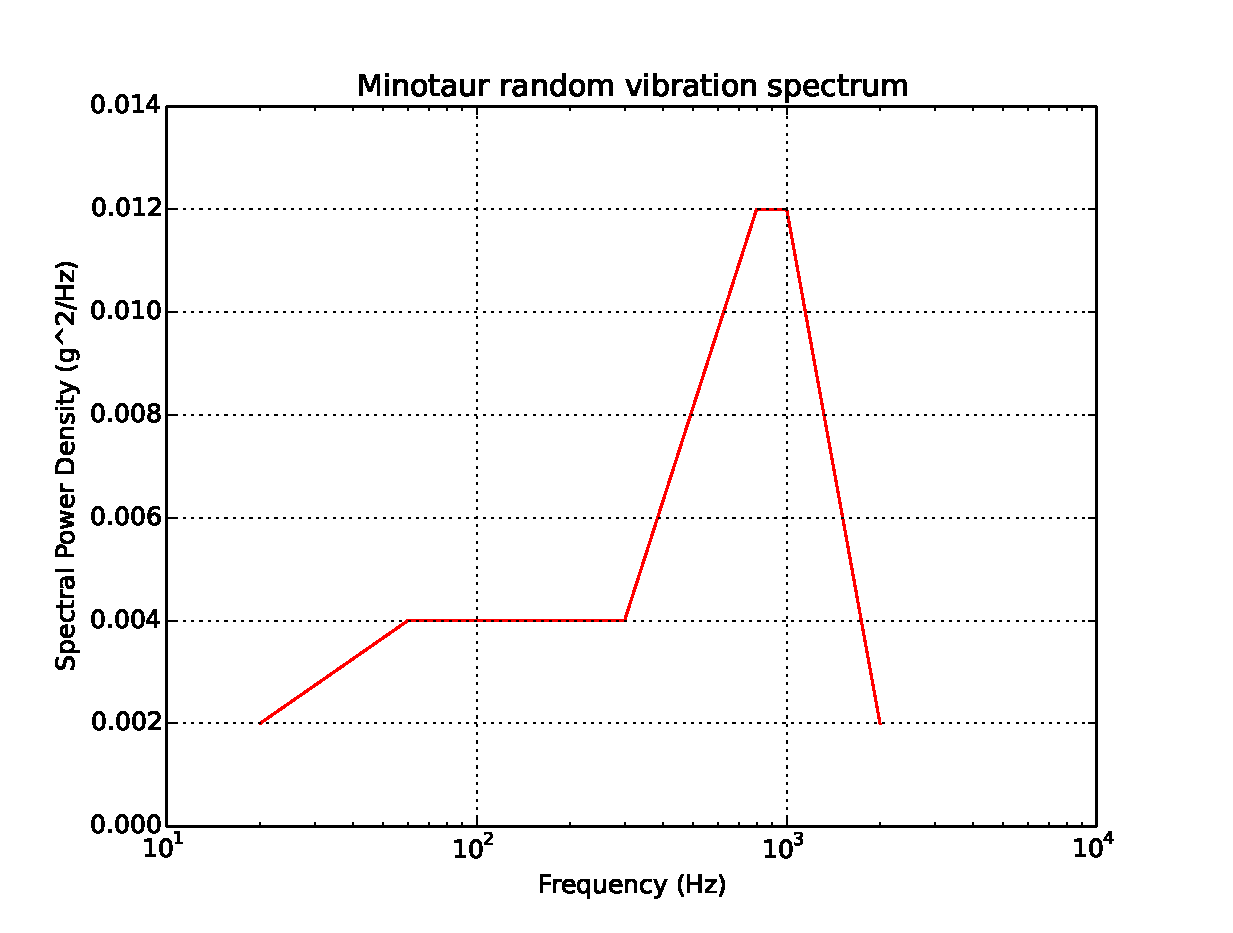
\includegraphics[width=1\textwidth]{Vibrations/Minotaur.eps} 
    \caption{Integral is 14.48 $g^2$, phase error is $1.2\degree$, for a crystal with a g-sensitivity of  1ppb/g.}
    \label{fig:MinotaurVibrations}
\end{figure}


\begin{figure}[!htb] 
    \centering
    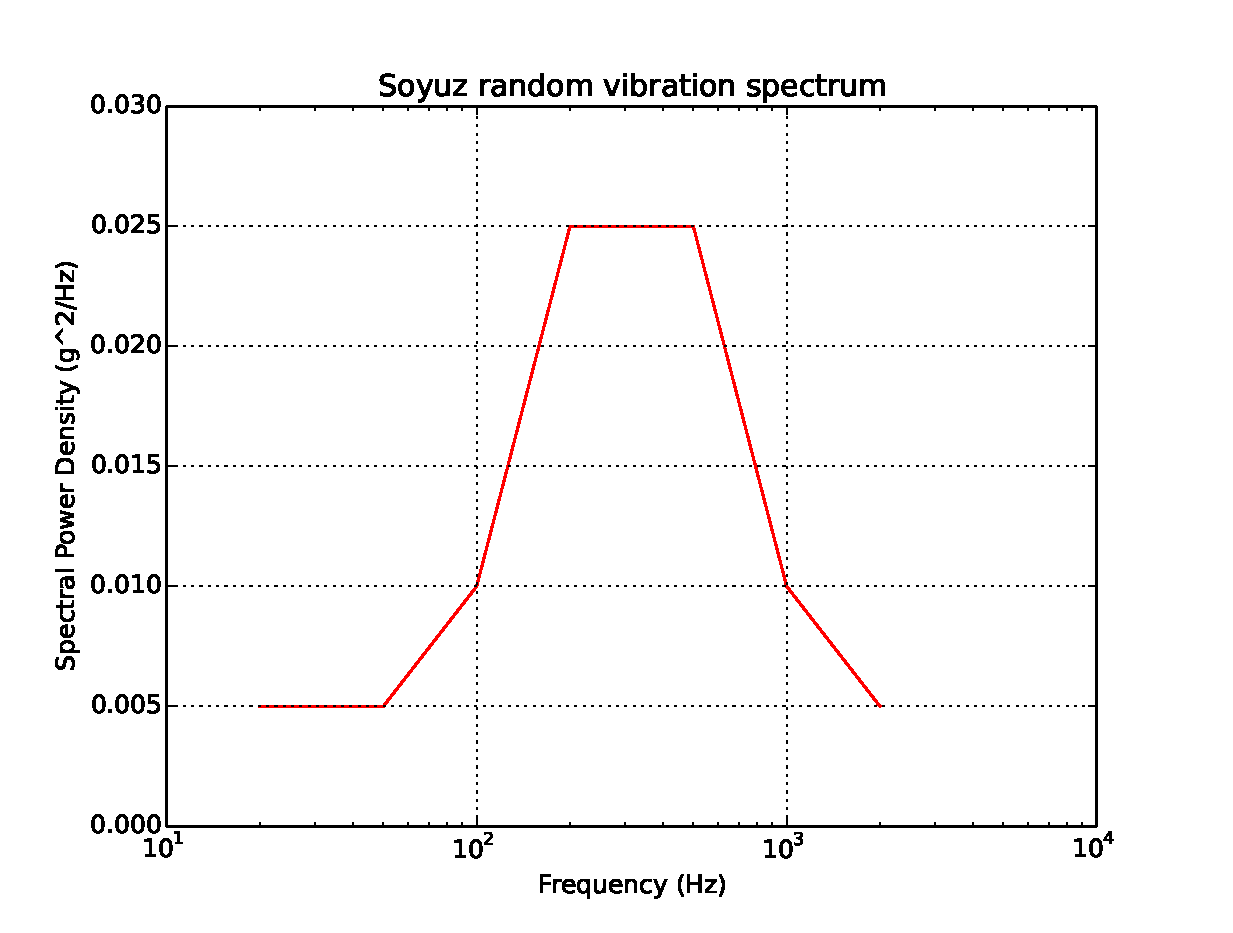
\includegraphics[width=1\textwidth]{Vibrations/Soyuz.eps} 
    \caption{Integral is 26.025 $g^2$, phase error is $1.8\degree$, for a crystal with a g-sensitivity of  1ppb/g.}
    \label{fig:SoyuzVibrations}
\end{figure}

\begin{figure}[!htb] 
    \centering
    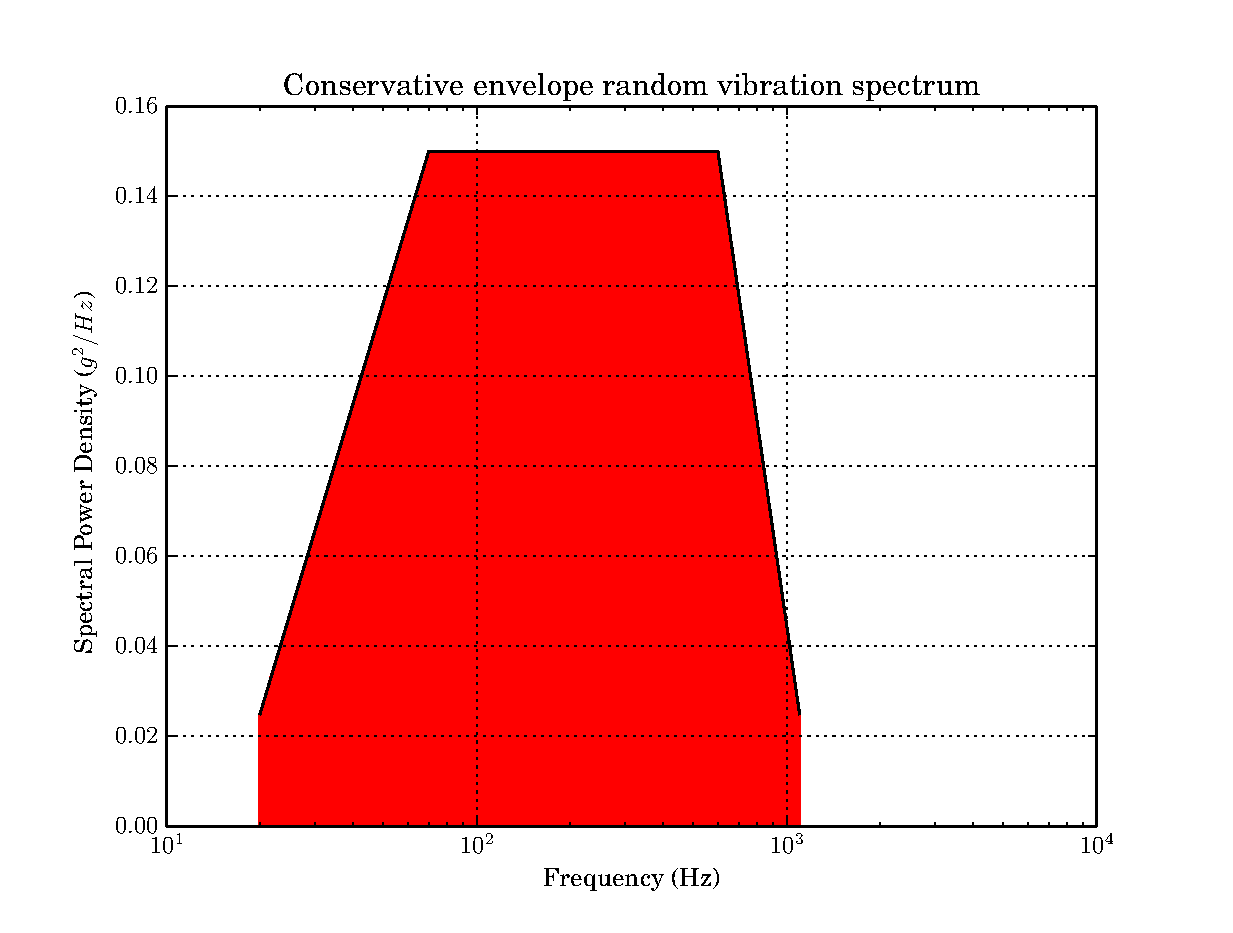
\includegraphics[width=1\textwidth]{Vibrations/Envelope.eps} 
    \caption{A conservative vibration spectrum envelope, from \cite{VibrationHandout}. Phase error is $5.9\degree$, for a crystal with a g-sensitivity of  1ppb/g.}
    \label{fig:ConservativeVibrations}
\end{figure}



\subsection{Shock stresses}
Space Exploration Technologies Corp  specifies four main shock events
\cite{Falcon9}: 
\begin{itemize}
\item{Vehicle hold-down release at lift-off} 
\item{2nd stage separation}
\item{Fairing separation}
\item{Payload release and separation}
\end{itemize}

\subsection{Acoustic stresses}


\subsection{Antenna phase-centre displacement}
One effect that is often overlooked, is that the antenna is physically displaced.


Equation 5.8
\begin{equation}
\sigma_v = \frac{360f_L}{2\pi}\sqrt{\int_{f_{min}}^{f_{max}} S^2_v(f_m) \frac{P(f_m)}{f^2_m} df_m}\text{ (degrees)}
\end{equation}
%\cite{Kaplan} \cite{Jwo}

Where:
\begin{align*}
f_L &= \text{L-band input frequency in Hz} \\
S_v(f_m) &= \text{oscillator vibration sensitivity of } \Delta f/f_L \text{ per g as a function of } f_m \\
f_m &= \text{random vibration modulation frequency in Hz} \\
P(f_m) &= \text{power curve of the random vibration in } g^2/Hz \text{ as a function of } f_m \\
g &= \text{ acceleration due to gravity } \approx 9.8 m/s^2\\
\end{align*}


Equation 5.16
Talk about the 2G tipover test
\begin{equation}
\Delta f_g = 360 S_g f_L G(t) (\degree/s)
\end{equation}
%\cite{Kaplan}

Where:
\begin{align*}
S_g &= \text{g-sensitivity of the oscillator } (\Delta \text{ f/f per g)}\\ 
f_L &= \text{L-band input frequency (Hz)}\\
&= \text{1,575.42 MHz for L1}\\
G(t) &= \text{acceleration stress in g as a function of time}
\end{align*}



%My work
%\addcontentsline{toc}{chapter}{Appendix 7}\label{app9}
\chapter{An Introduction to Tracking Loops}
In summary, the goal of the carrier tracking loop is to predict the future carrier phase $\phi$,$T$ seconds in the future, based on past and current measurements of the carrier phase. For successful phase lock to be maintained, the predicted phase must be within a small fraction of a cycle of the actual phase. 

\section{Ambiguities}

We can describe the elapsed phase (in radians) between the satellite and the receiver using the following equation :  
\begin{equation}
Phase = 2 \pi N  + \phi 
\label{eq:Phase}
\end{equation}

If we examine equation \ref{eq:Phase} in the spatial domain, we find that: 
\begin{equation}
Range = \lambda N + \Phi
\label{eq:Distance}
\end{equation}

From Equations \ref{eq:Phase} and \ref{eq:Distance} it is obvious that prediction of the angular phase $\phi$ is equivalent to prediction of the spatial phase $\Phi$.

It is important to note, that predicting $\Phi$ is equivalent to predicting the change in the LOS range ($\Delta$), hence the receiver does not need to be aware of the number of full cycles $N$, between it and the satellite. This ambiguity is the one that is resolved during the process of carrier phase positioning. 

\section{Error bounds}
In the case of the GPS signal, where the $L_1$ 1.575Ghz signal is being tracked, the carrier wavelength, $\lambda \approx 19.03 cm$ long. As a heuristic, the difference between the actual carrier phase $\phi$ , and the predicted carrier phase $\hat{\phi}$ must be no more than $\pm30 \degree$. 

This concept is clearly illustrated in figure \ref{fig:PhaseDelay}. 

Denoting our prediction of $\Delta$ as $\hat{\Delta}$, we have :

\begin{align}
|\Delta-\hat{\Delta}|& < \frac{30\degree}{360\degree} \lambda\\
|\Delta-\hat{\Delta}|&<\epsilon\\
|\Delta-\hat{\Delta}|&<1.58cm\\
\label{eq:RangeErrorBound}
\end{align}

Hence, our estimate of $\Delta$ must be accurate to $< 1.58cm$, if the receiver is to remain in phase lock.

By examining figure \ref{fig:ValidPositions} we can begin to understand that the locus of all possible positions which meet this criteria is a spherical shell surrounding the satellite. 

When we consider that GPS utilises multiple satellites for positioning, we can conclude with the aid of figure \ref{fig:Intersections} that a bound on the magnitude of the error is formed by the sphere of radius $\epsilon$ surrounding the point X, which is the true position of the receiver. 

Hence, we have :

\begin{comment}
\begin{align}
| X(t)-\hat{X}(t) | & < \frac{30\degree}{360\degree} \lambda \\
| X(t)-\hat{X}(t) | &<\Delta\\
| X(t)-\hat{X}(t) | & < 1.58cm
\label{eq:PositionErrorBound}
\end{align}
\end{comment}

\section{Mechanics}

By conceptualising we can immediately gain insight into some of the fundamental challenges that will be faced in the development of tracking algorithms for coping with high dynamics.

\tikzset{
block/.style = {draw, fill=white, rectangle, minimum height=3em, minimum width=3em},
tmp/.style  = {coordinate}, 
sum/.style= {draw, fill=white, circle, node distance=1cm},
input/.style = {coordinate},
output/.style= {coordinate},
pinstyle/.style = {pin edge={to-,thin,black}
}
}

\begin{figure}[!htb]
\centering

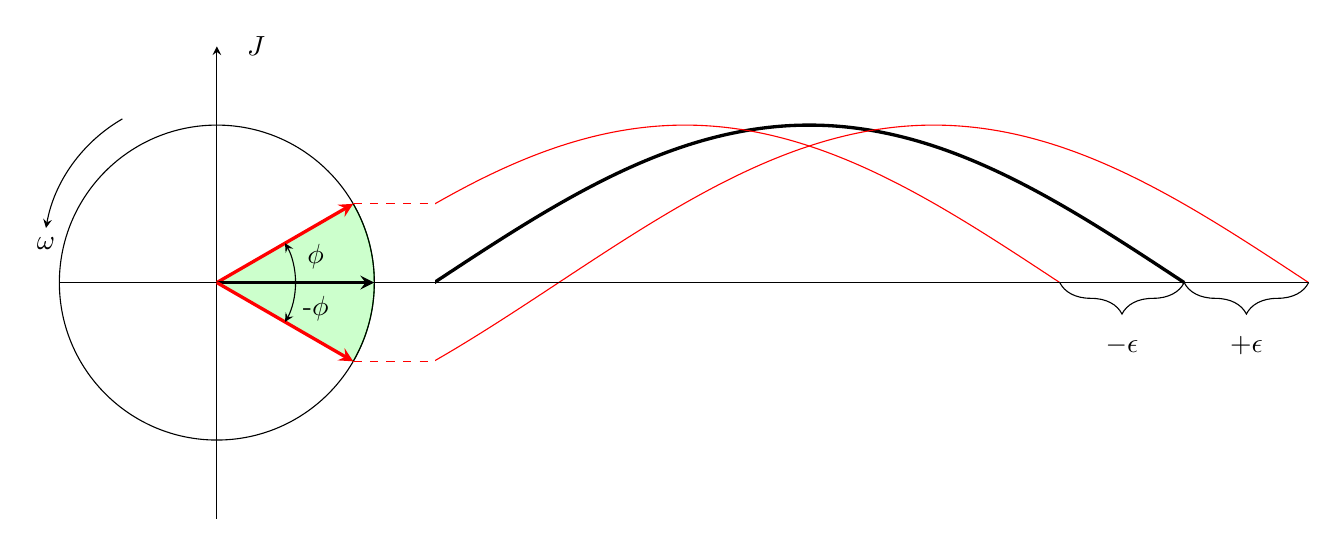
\begin{tikzpicture}
    
    \draw[black,very thick] (4.76175-2,0) sin (2*4.76175-2,2) cos (3*4.76175-2,0) ;
    
    \draw[red] (4.76175-1.58-2,0) sin (2*4.76175-1.58-2,2) cos (3*4.76175-1.58-2,0) ;
    
    \draw[red] (1.58-2,-2) cos (4.76175+1.58-2,0) sin (2*4.76175+1.58-2,2) cos (3*4.76175+1.58-2,0) ;
    
    \draw [decorate,decoration={brace,amplitude=0.4cm},xshift=0,yshift=0pt]
(3*4.76175+1.58-2,0) -- (3*4.76175-2,0) node [black,midway]{};
    \node at (3*4.76175+0.5*1.58-2,-0.8) {$+\epsilon$};
    
    \draw [decorate,decoration={brace,amplitude=0.4cm,mirror},xshift=0,yshift=0pt]
(3*4.76175-1.58-2,0) -- (3*4.76175-2,0) node [black,midway]{};

    \node at (3*4.76175-0.5*1.58-2,-0.8) {$-\epsilon$};

    \draw [fill opacity=1, fill=white,white] (-1.58,2) rectangle(2.76175,-2);
    
    \filldraw[fill=green!20!white, draw=green!50!black]
    (0,0) -- (-30:2) arc (-30:30:2) -- cycle;
    \draw (0,0) circle (2cm);
    
    \draw[->,-stealth,color=black] (0,-3) -- (0,3);
    \node at (0.5,3) {$J$};
    
    \draw(-2,0) -- (3*4.76175+1.58-2,0);
    
    \draw[->,color=red, very thick,-stealth] (0,0)--(30:2);
    \draw[->,color=black, very thick,-stealth ] (0,0)--(0:2);
    \draw[->,color=red, very thick,-stealth ] (0,0)--(-30:2);
    
    \draw[-,color=red, dashed] (30:2)--(2.76175,1);
    \draw[-,color=red, dashed] (-30:2)--(2.76175,-1);
    
    \draw[->,-stealth ]  (0:1cm) arc (0:30:1cm);
    \draw[->,-stealth ]  (0:1cm) arc (0:-30:1cm);
    
    \node at (15:1.3) {$\phi$};
    \node at (-15:1.3) {-$\phi$};
    % angular velocity \omega
    \draw[->,-stealth ]  (120:2.4cm) arc (120:170:2) node[below] {$\omega$};
    
    \end{tikzpicture}
\caption{A scale drawing of the tolerances required for successful phase lock of the GPS $L_1$ signal. The phase, $\phi$ of the locally generated carrier (red) needs to remain within $30\degree$ of the phase the incoming carrier (black). This equates to a $\Delta$ range of 1.58 cm to the satellite.} \label{fig:PhaseDelay}
\end{figure}


\tikzset{
block/.style = {draw, fill=white, rectangle, minimum height=3em, minimum width=3em},
tmp/.style  = {coordinate}, 
sum/.style= {draw, fill=white, circle, node distance=1cm},
input/.style = {coordinate},
output/.style= {coordinate},
pinstyle/.style = {pin edge={to-,thin,black}
}
}

\begin{figure}[!htb]
\centering

\begin{tikzpicture}
    \newcommand\Radius{6} 
    \filldraw[fill=green!20!white, draw=green!50!black]
    (0:\Radius+1.58) arc (0:360:\Radius+1.58) -- cycle;
    
    \filldraw[fill=white, draw=green!50!black]
    (0:\Radius-1.58) arc (0:360:\Radius-1.58) -- cycle;
    
    \draw[draw=green!50!black,dashed]
    (0:\Radius) arc (0:360:\Radius) -- cycle;
    
    \draw[->,color=black,-stealth, thick] (0,0)--(30:\Radius+1.58);
    \draw[->,color=black,-stealth, thick] (0,0)--(90:\Radius);
    \draw[->,color=black,-stealth, thick] (0,0)--(150:\Radius-1.58);
    
    
    \node at (20:3) {$r+\Delta$};
    \node at (95:3) {$r$};
    \node at (160:3) {$r-\Delta$};
    \node at (0,-0.25) {Satellite};
    
    \end{tikzpicture}
\caption{In order to maintain phase lock with a single satellite, the predicted range to the satellite used to generate the phase, must lie inside an spherical shell, centred around the true range to the satellite. The shell is visualised as an annulus which is bounded by $r-\epsilon<r<r+\epsilon$. $\epsilon$ is depicted at 1:1 scale.} \label{fig:ValidPositions}
\end{figure}


\tikzset{
block/.style = {draw, fill=white, rectangle, minimum height=3em, minimum width=3em},
tmp/.style  = {coordinate}, 
sum/.style= {draw, fill=white, circle, node distance=1cm},
input/.style = {coordinate},
output/.style= {coordinate},
pinstyle/.style = {pin edge={to-,thin,black}
}
}

\begin{figure}[!htb]
\centering

\begin{tikzpicture}
    %\filldraw[fill=green!20!white, draw=green!20!white]
    %(-59.5:7.58) arc (-59.5:-120.5:7.58) arc (147:32:4.58) %--cycle;
    
    \filldraw[fill=green!20!white, draw=green!20!white]
    (-46:5.58) arc (-46:-134:5.58) arc (134.5:46:5.58);
    
    
    \newcommand\RadiusA{4} 
    \draw[draw=black]
    (0:\RadiusA+1.58) arc (0:360:\RadiusA+1.58) -- cycle;
    
    \draw[draw=black]
    (0:\RadiusA-1.58) arc (0:360:\RadiusA-1.58) -- cycle;
    
    \draw[draw=black,dashed]
    (0:\RadiusA) arc (0:360:\RadiusA) -- cycle;
    
    \node at (0,0) {Satellite A};
    
    \newcommand\RadiusB{4} 
    \draw[draw=black]
    (\RadiusB+1.58,-8) arc (0:360:\RadiusB+1.58) -- cycle;
    
    \draw[draw=black]
    (\RadiusB-1.58,-8) arc (0:360:\RadiusB-1.58) -- cycle;
    
    \draw[dashed]
    (\RadiusB,-8) arc (0:360:\RadiusB) -- cycle;
    
    \node at (0,-8) {Satellite B};
    
    \node at (0,-4.35) {$X$};
    
    \end{tikzpicture}
\caption{In the case of multiple satellites, the only viable positions where phase lock can be maintained is the union between the spherical shells of the satellites, visualised here as annuli. As the number of different satellites increases, the bounding volume of the solution approaches a sphere with radius 2 $\epsilon$ centred at the true position X. $\epsilon$ is depicted at 1:1 scale.}
\label{fig:Intersections}
\end{figure}



Returning to first principles of mechanics, we have \cite{salas1999etgen} : 

\begin{comment}
Need to fix this up
\end{comment}

\begin{align}
v & = \frac{\Delta}{T} m s^{-1} \\
a & = \frac{dv}{dt} m s^{-2} \\
Jerk & = \frac{da}{dt} m s^{-3}
\end{align}


Note that over time, the acceleration of the receiver is integrated to form it's velocity, and the velocity is integrated in order to form it's position. 

Note that our estimate of the position $\hat{X}(t+T)$ is dependent on our current velocity $\dot{X}(t)$. When use this velocity, we are implicit assuming that the average velocity for the next time period is the same. 

However,as illustrated in figure \ref{fig:PhaseDelay}, and in equation \ref{eq:RangeErrorBound}, our estimate of the new range to the satellite must fall within 
position must fall within a close 

our estimate of the velocity must fall within the following bounds:



\begin{equation}
V_{min} < \hat{\dot{X}}(t) < V_{max}
\end{equation}





\section{Motion Models}

Given we are attempting to predict the carrier $T$ seconds into the future, we can start to investigate the maximum dynamics our receiver will be able to track for a given sampling period $T$. \cite{salas1999etgen}


\begin{equation}
X = \int_{t_1}^{t_2} \dot{X} dt + X(t_1)
\label{eq:PositionIntergral}
\end{equation}

\begin{equation}
\dot{X} = \int_{t_1}^{t_2} \ddot{X} dt + \dot{X}(t_1)
\end{equation}


Equation \ref{eq:PositionIntergral} suggests that we can form an prediction of the range to the satellite using the current range and the current line of sight velocity. 

\begin{equation}
\hat{X}(t+T) = X(t) +  \dot{X}(t) T
\end{equation}

\begin{equation}
t = nT
\end{equation}

\begin{equation}
\hat{X}[n+1] = X[n] +  \dot{X}[n] T
\end{equation}




\section{Kaplan Stuff}
Kaplan suggests that "A conservative rule of thumb for tracking threshold is that the 3-sigma jitter must not exceed one-fourth of the phase pull-in range of the PLL discriminator." \cite{Kaplan}

\begin{equation}
3 \sigma_{PLL} = 3 \sigma_j +\theta_e \leq 45 \degree
\end{equation}

Where:
\begin{framed}
$\sigma_j$ = 1-sigma phase jitter from all sources except dynamic stress error \\
$\theta_e$ = dynamic stress error in the PLL tracking loop
\end{framed}
\cite{Kaplan}

Equation 5.5
\begin{equation}
\sigma_{PLL} = \sqrt{\sigma^2_{tPLL} + \sigma^2_v+ \theta^2_A} + \frac{\theta_e}{3} \leq 15 \degree 
\end{equation}
\cite{Jwo}

where
\begin{framed}
$\sigma_{tPLL}$ = 1-sigma thermal noise in degrees \\
$\sigma_v$ = 1-sigma vibration-induced oscillator jitter in degrees \\
$\theta_A$ = Allan variance induced oscillator jitter in degrees
\end{framed}
\cite{Kaplan}\cite{Jwo}

Equation 5.6
\begin{equation}
\sigma_{PLLt} = \frac{360}{2 \pi} \sqrt{\frac{B_n}{C/N_0}(1+\frac{1}{2TC/N_0})} (degrees)
\end{equation}
\cite{Kaplan}


Equation 5.7
\begin{equation}
\sigma_{PLLt} = \frac{\lambda_L}{2 \pi} \sqrt{\frac{B_n}{C/N_0}(1+\frac{1}{2TC/N_0})} (m)
\end{equation}
\cite{Kaplan}

where:
\begin{framed}
$B_n$ = carrier loop noise bandwidth (Hz) \\
$C/N_0$ = carrier to noise power ratio in (Hz) \\
= $10^\frac{(C/N_0)_dB}{10}$ \\
T = predetection (coherent) integration time (s) \\
$\lambda_L$ = GPS L1 carrier wavelength (m)
= 0.1903 m
\end{framed}
\cite{Kaplan} \cite{Jwo}


Equation 5.8
\begin{equation}
\sigma_v = \frac{360f_L}{2\pi}\sqrt{\int_{f_{min}}^{f_{max}} S^2_v(f_m) \frac{P(f_m)}{f^2_m} df_m} (degrees)
\end{equation}
\cite{Kaplan} \cite{Jwo}

where
\begin{framed}
$f_L$ = L-band input frequency in Hz \\
$S_v(f_m)$ = oscillator vibration sensitivity of $\Delta f/f_L$ per g as a function of $f_m$ \\
$f_m$ = random vibration modulation frequency in Hz \\
$P(f_m)$ = power curve of the random vibration in $g^2/Hz$ as a function of $f_m$ \\
g = acceleration due to gravity $\approx 9.8 m/s^2$
\end{framed}

(Perhaps an appendix on vibrations?)

Equation 5.16
Talk about the 2G tipover test
\begin{equation}
\Delta f_g = 360 S_g f_L G(t) (\degree/s)
\end{equation}
\cite{Kaplan}

$S_g$ = g-sensitivity of the oscillator ($\Delta$ f/f per g) 
$f_L$ = L-band input frequency (Hz)
= 1,575.42 MHz for L1
G(t) = acceleration stress in g as a function of time


Talk about this
5.6.2 FLL Tracking Loop Measurement Errors

Generate figure 5.24
Generate figure 5.25

Also talk about section 5.6.2






















\begin{comment}
This document provides and overview of the Namuru carrier tracking loop architecture. The software architecture has evolved over time, and uses elements of different approaches from the literature, as well as a number of novel components implemented by Dr Eamonn Glennon. 

\section{Current Namuru architecture}

The Namuru receiver currently uses a third-order PLL loop filter with a second-order FLL assist. This architecture can be seen in figure .  A third order PLL uses a second order filter, with the third integrator being the VCO.

Namuru additionally has a code tracking loop, however will not be discussed in this document. The dynamics experienced by the code tracking loop are 1540 times smaller than those experienced by the carrier loop \cite{Kaplan}. Hence the  code loop is significantly more robust than either the FLL or PLL.

The PLL is the most vulnerable of the loops, and under extreme dynamics, the PLL will break and the FLL will keep tracking, before the PLL resumes tracking once the dynamics have subsided to more reasonable levels. Hence, while the FLL is described, more effort will be expended on analysis of the PLL.

\section{Tracking Loops}

The receiver implements a digital (sampled) phase lock loop (PLL), the theoretical background of which is covered thoroughly in Gardner \cite{Gardner}. 
 
Additionally, the receiver also implements a FLL, which is used to assist the PLL in locking.

Both of the loops include a number of components that will be discussed in more detail later, 

\begin{itemize}
\item{Discriminator}
\item{Integrate \& Dump}
\item{Loop Controller/Loop Filter}
\item{Hold}
\item{Delay}
\item{NCO}
\end{itemize}

In the they key difference between the two filters is the discriminator. 
\end{comment}
%Simulator Jitter




 